\section{Results}
\label{sec:results}

\begin{figure}[htbp]
\begin{center}
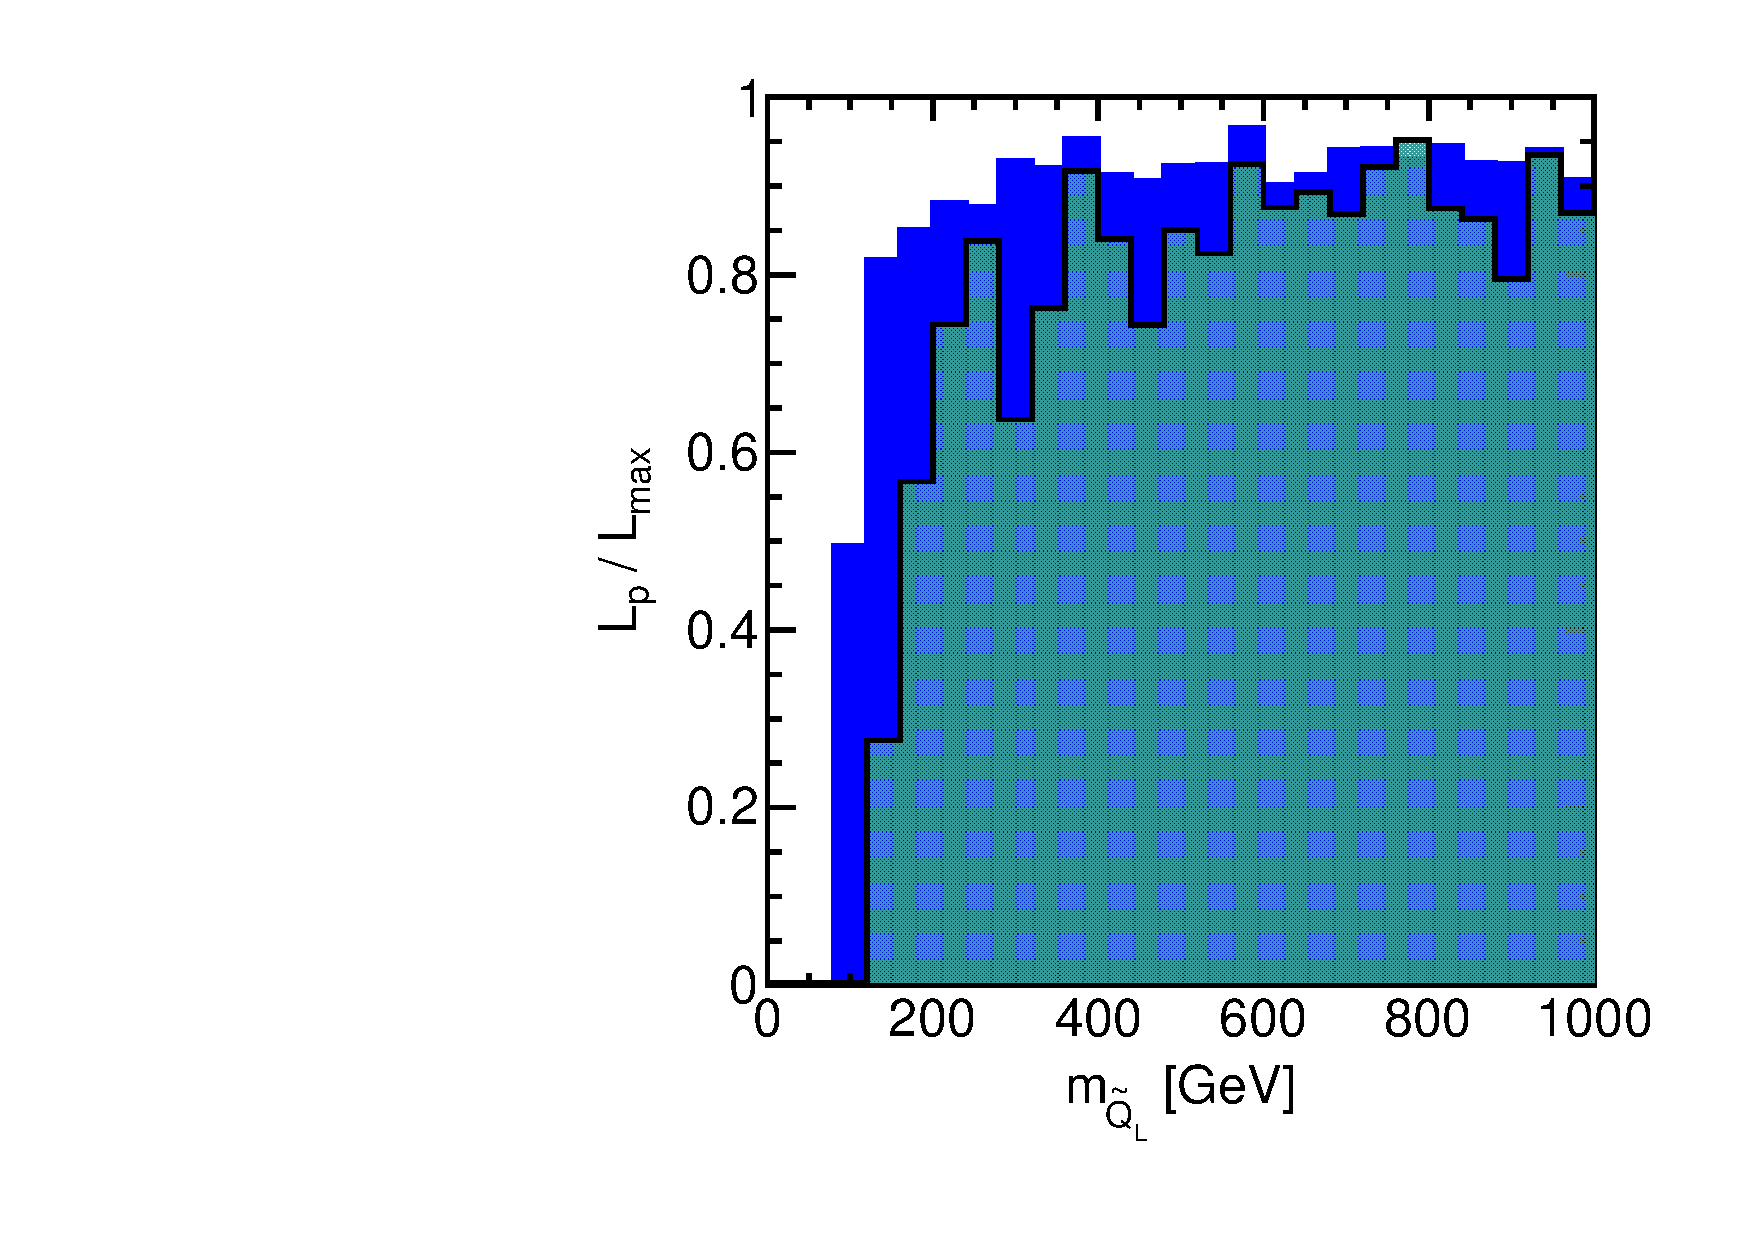
\includegraphics[height=5.5cm]{figs/fig_m_Q_L.pdf} 
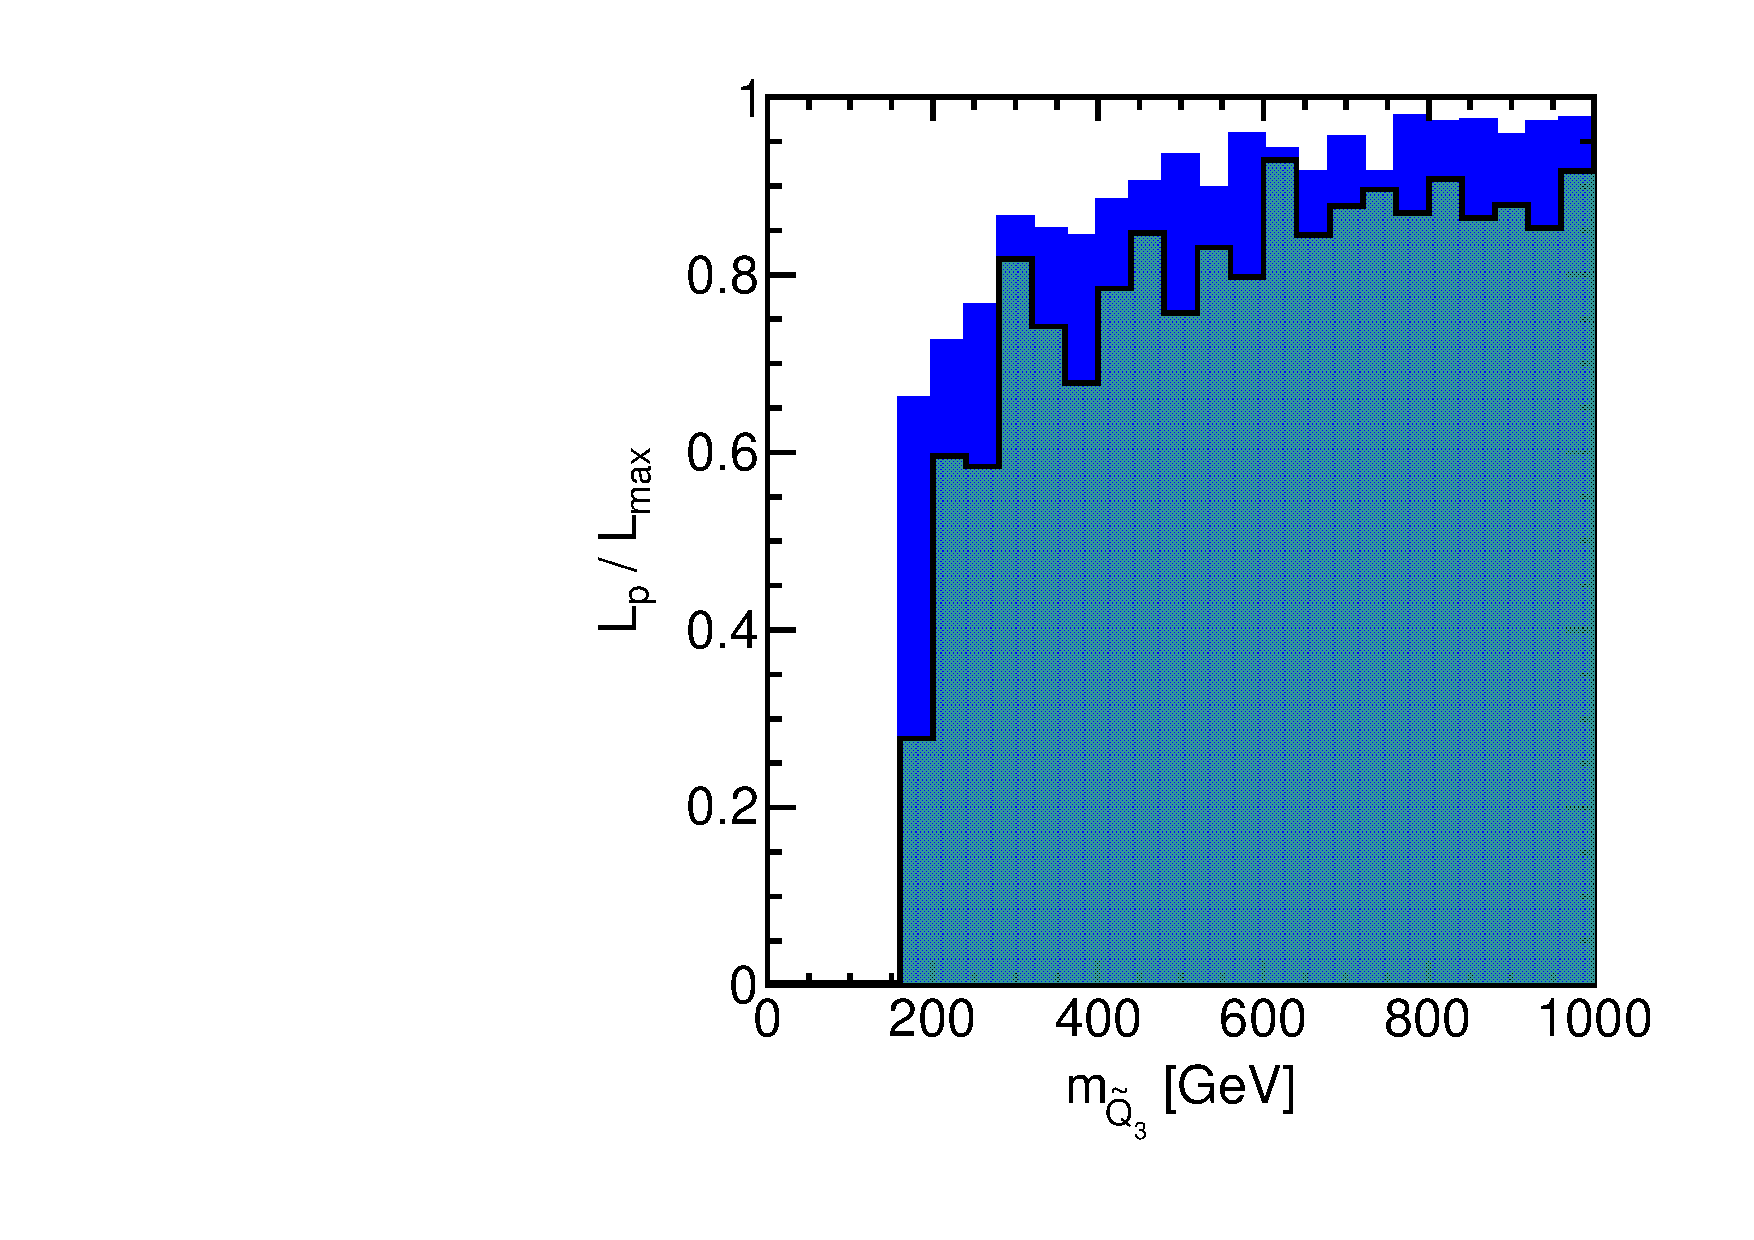
\includegraphics[height=5.5cm]{figs/fig_m_Q_3.pdf} \\
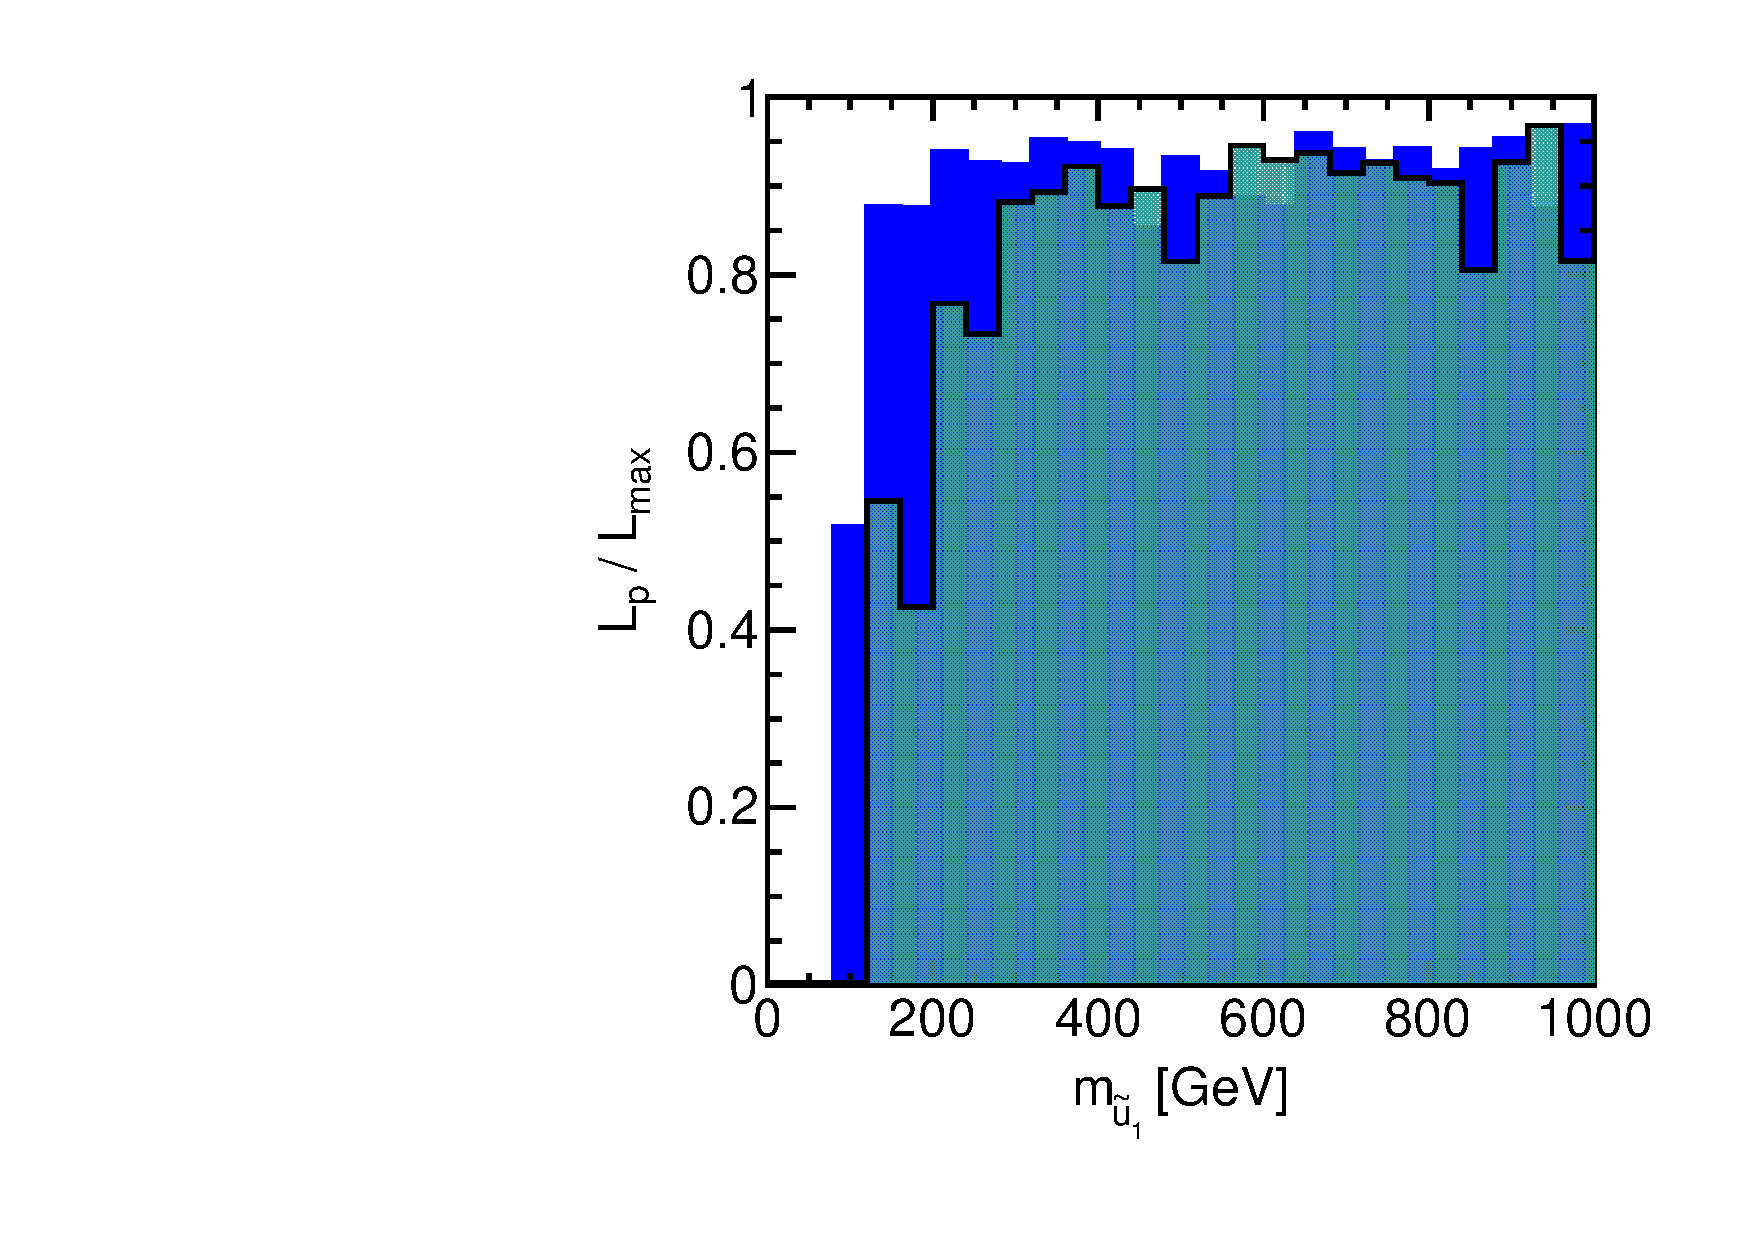
\includegraphics[height=5.5cm]{figs/fig_m_u_1.pdf}
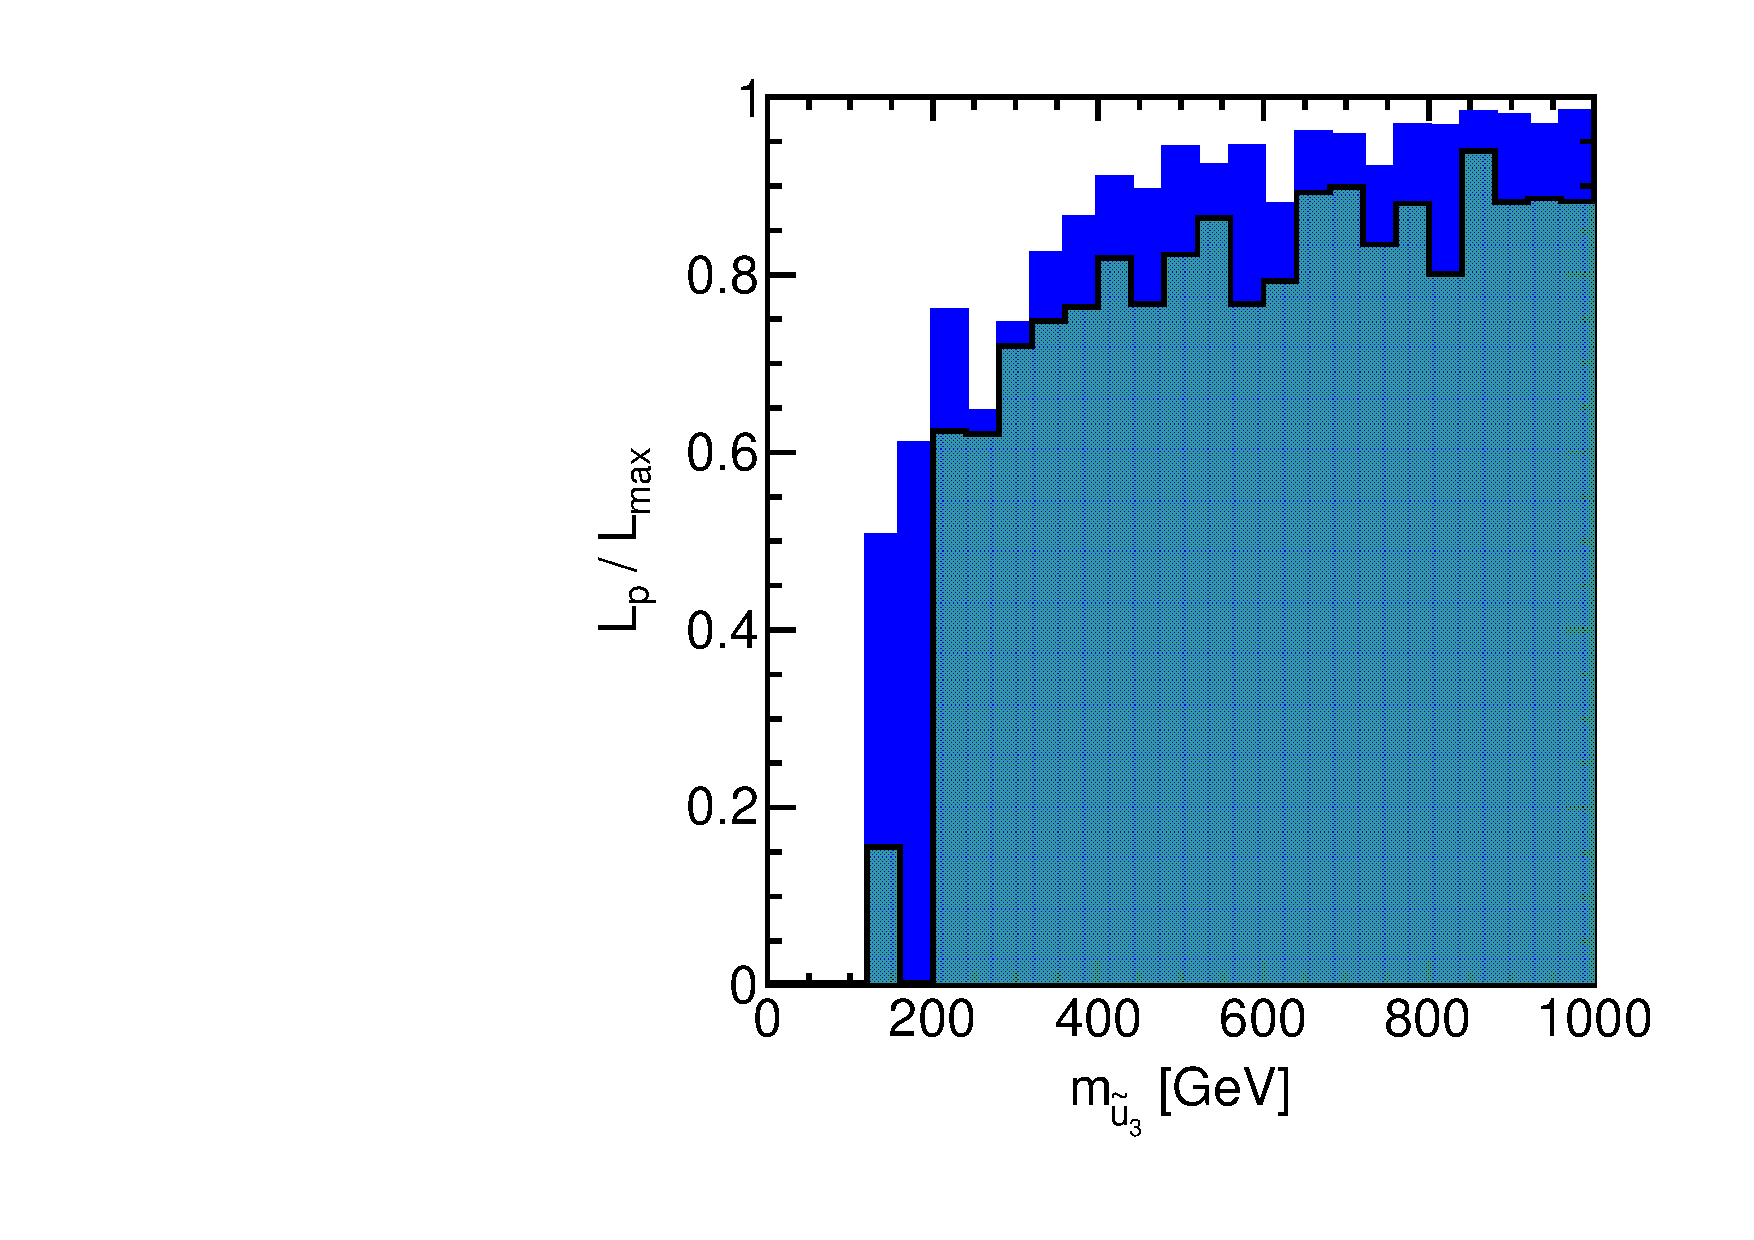
\includegraphics[height=5.5cm]{figs/fig_m_u_3.pdf} \\
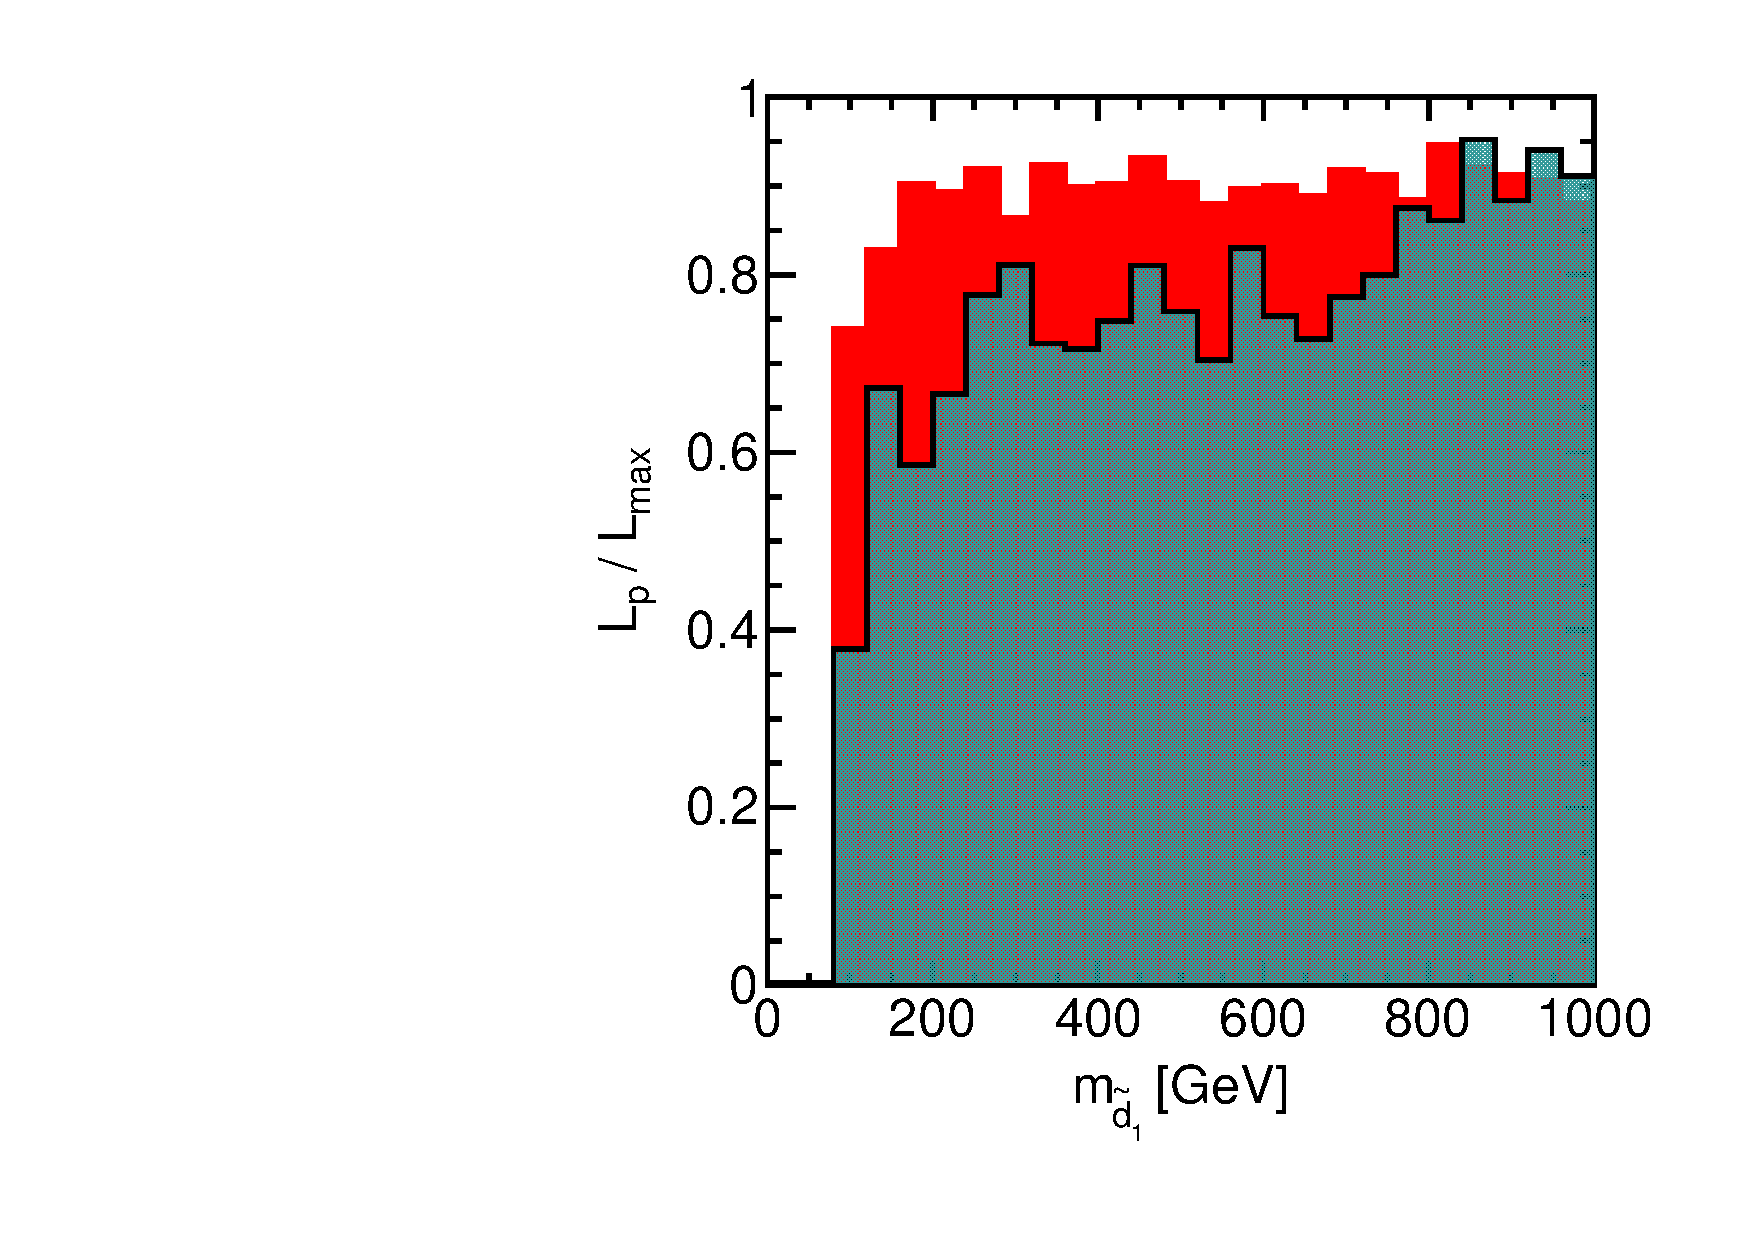
\includegraphics[height=5.5cm]{figs/fig_m_d_1.pdf}
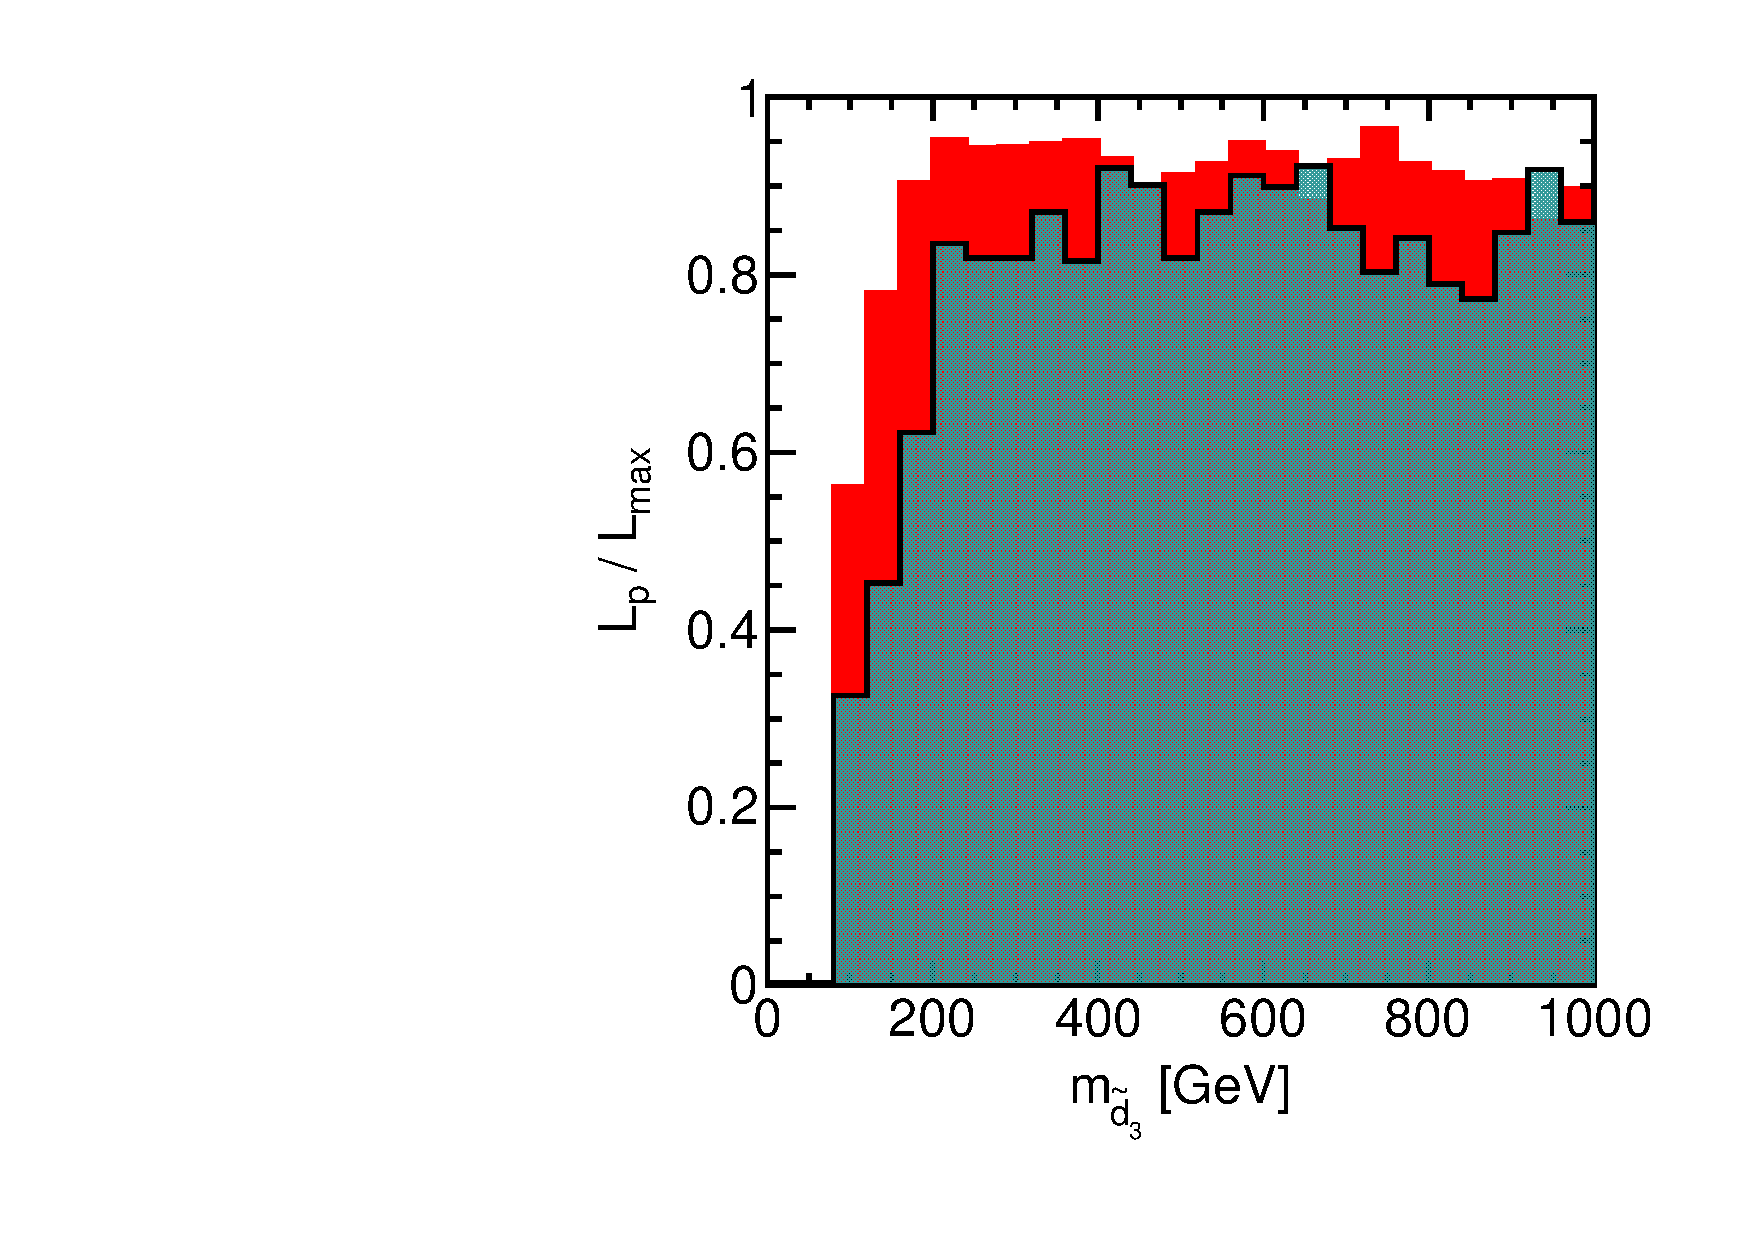
\includegraphics[height=5.5cm]{figs/fig_m_d_3.pdf}
\caption{Squark mass parameters at the SUSY scale}
\label{default}
\end{center}
\end{figure}


\begin{figure}[htbp]
\begin{center}
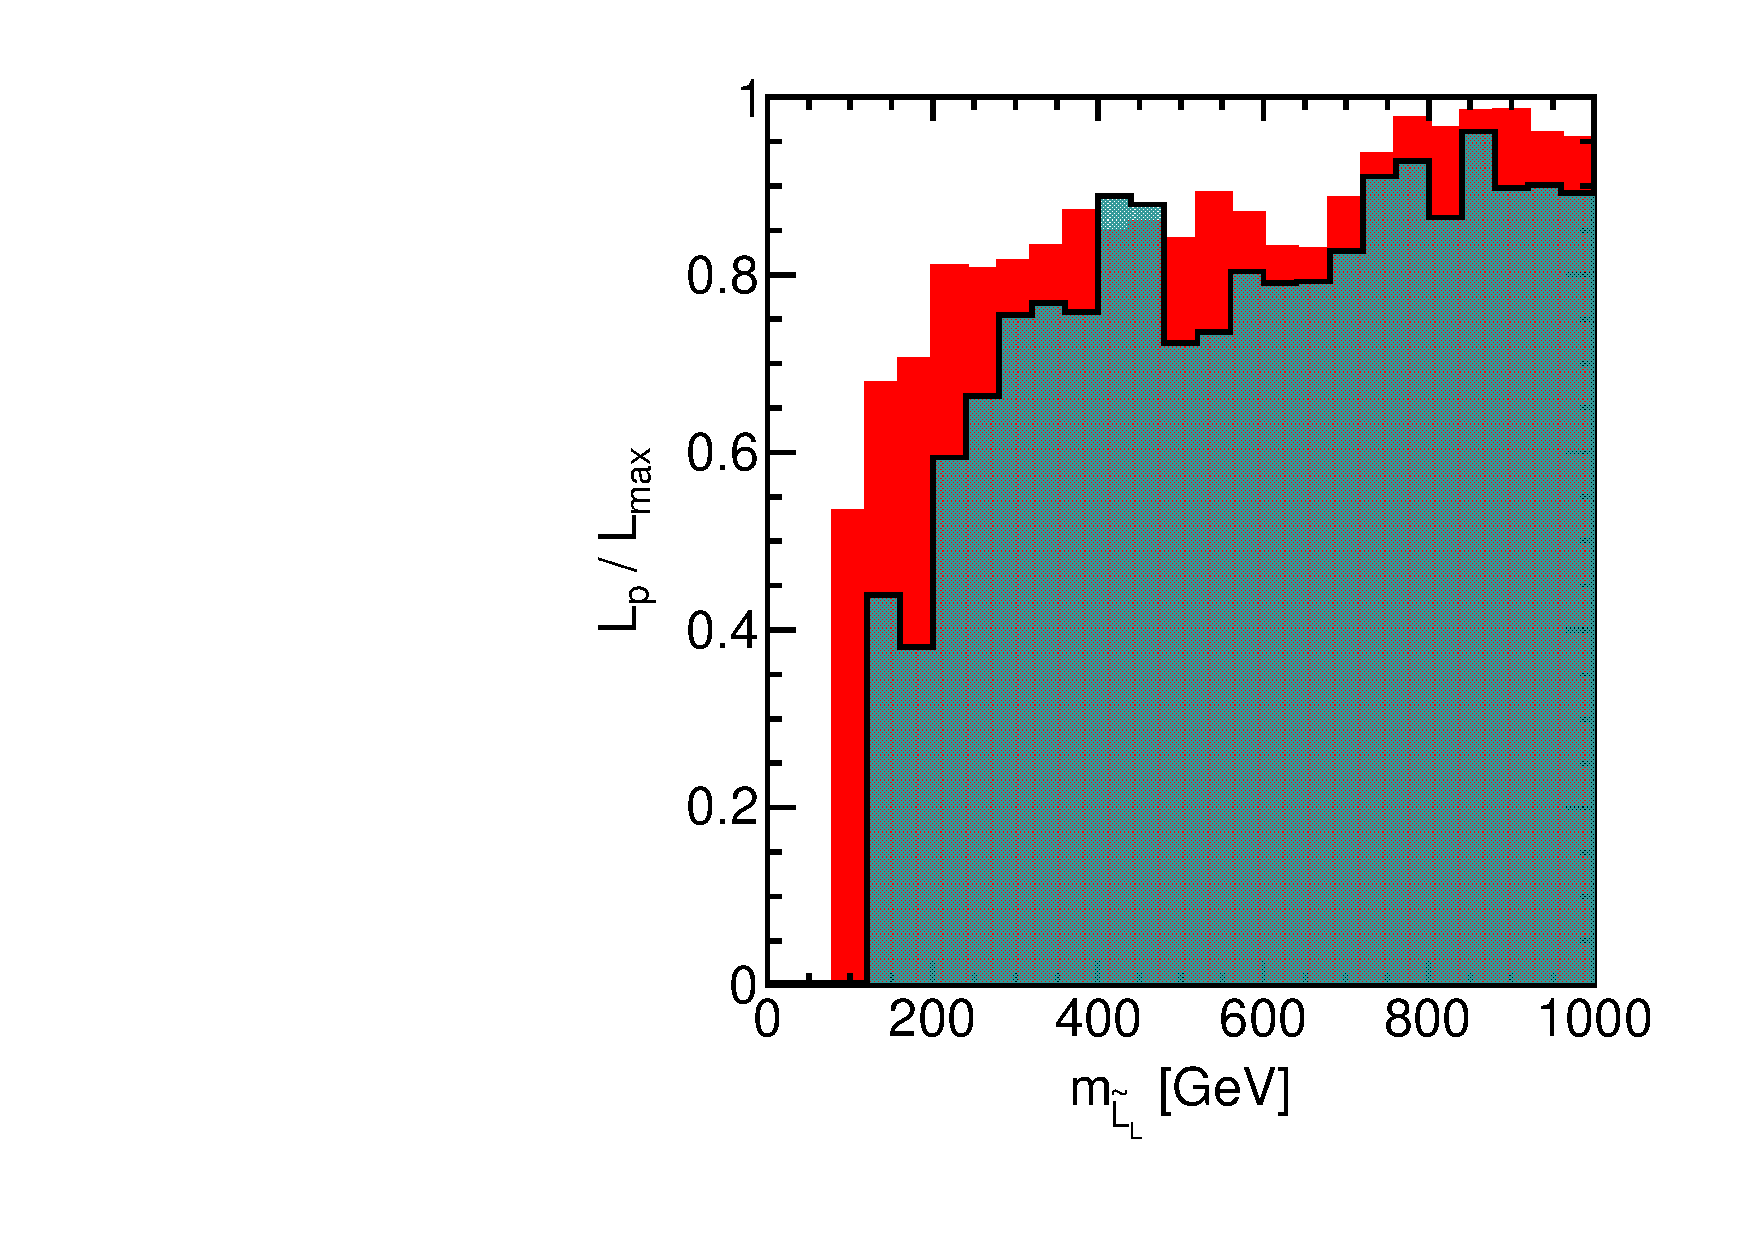
\includegraphics[height=5.5cm]{figs/fig_m_L_L.pdf} 
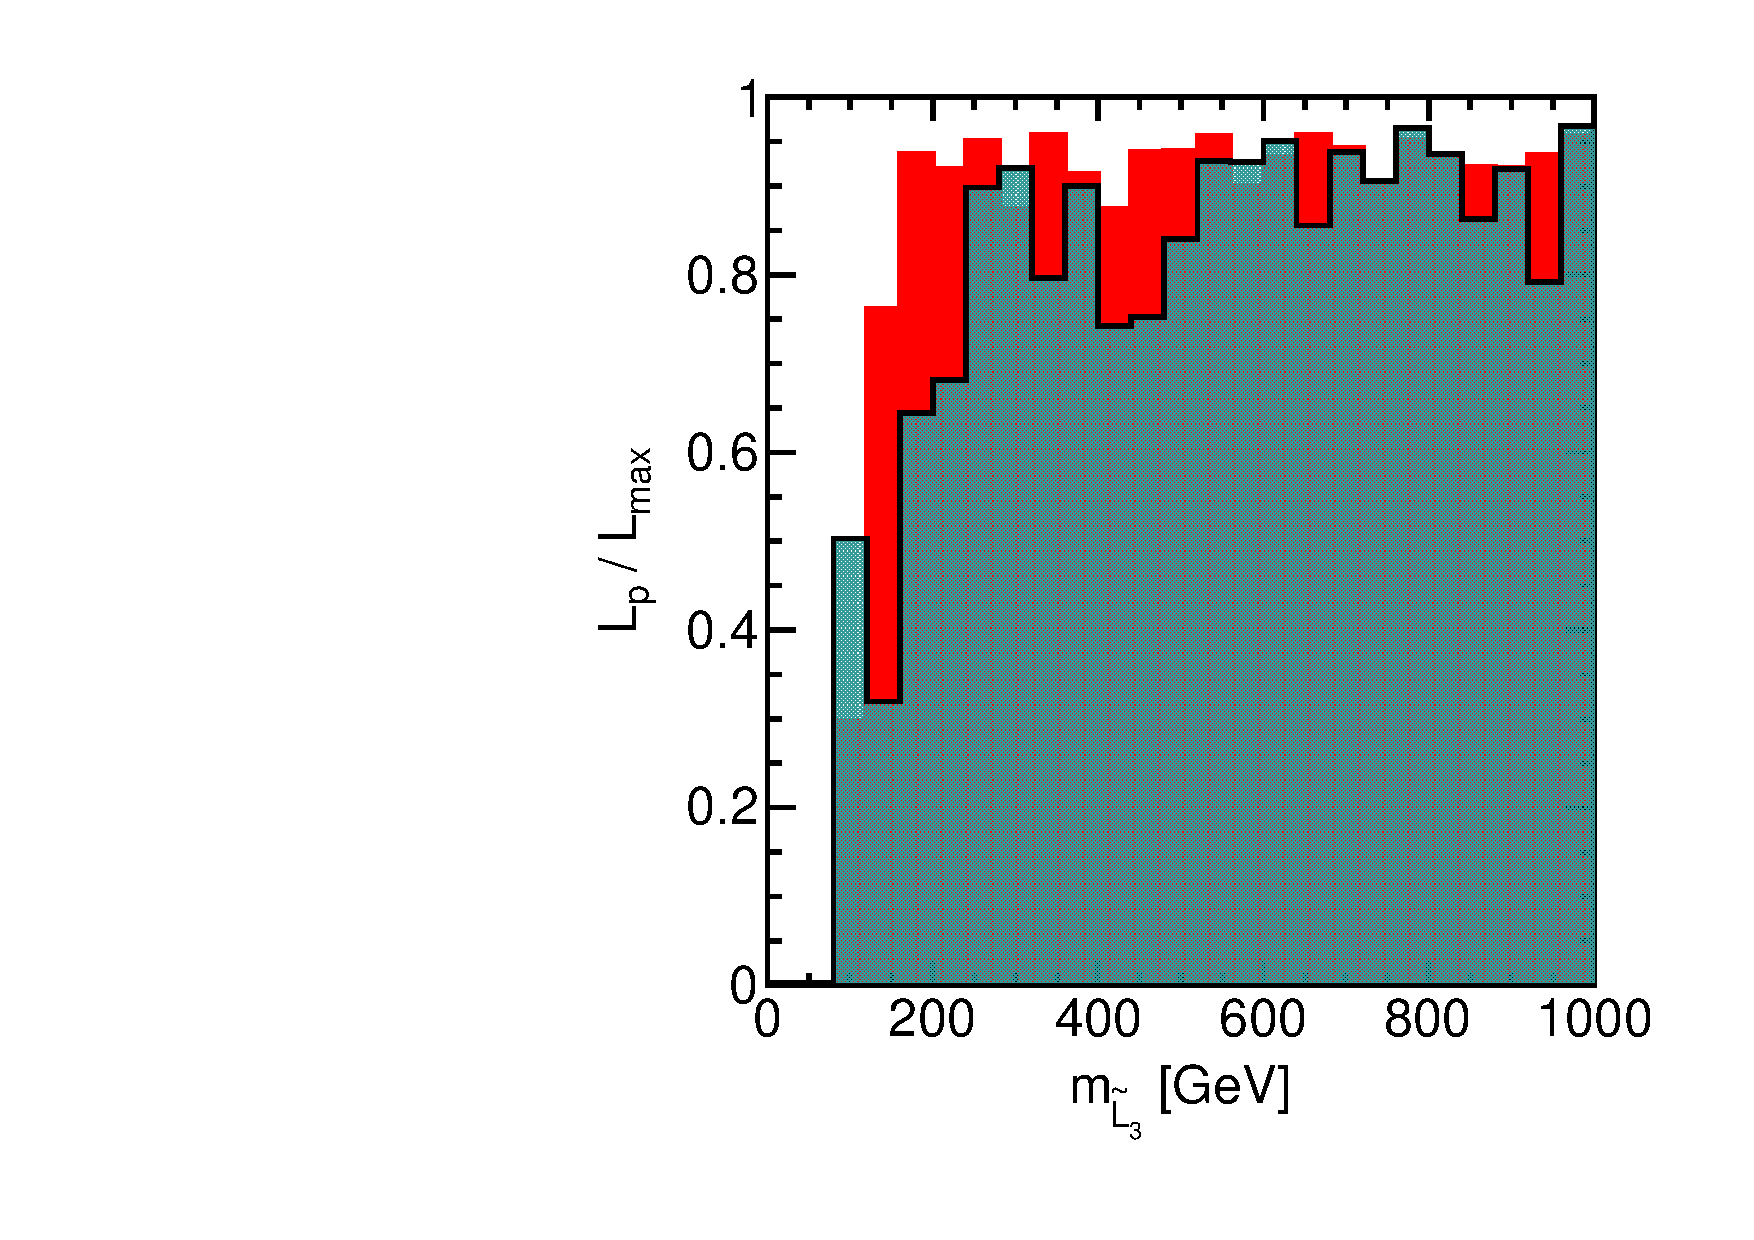
\includegraphics[height=5.5cm]{figs/fig_m_L_3.pdf} \\
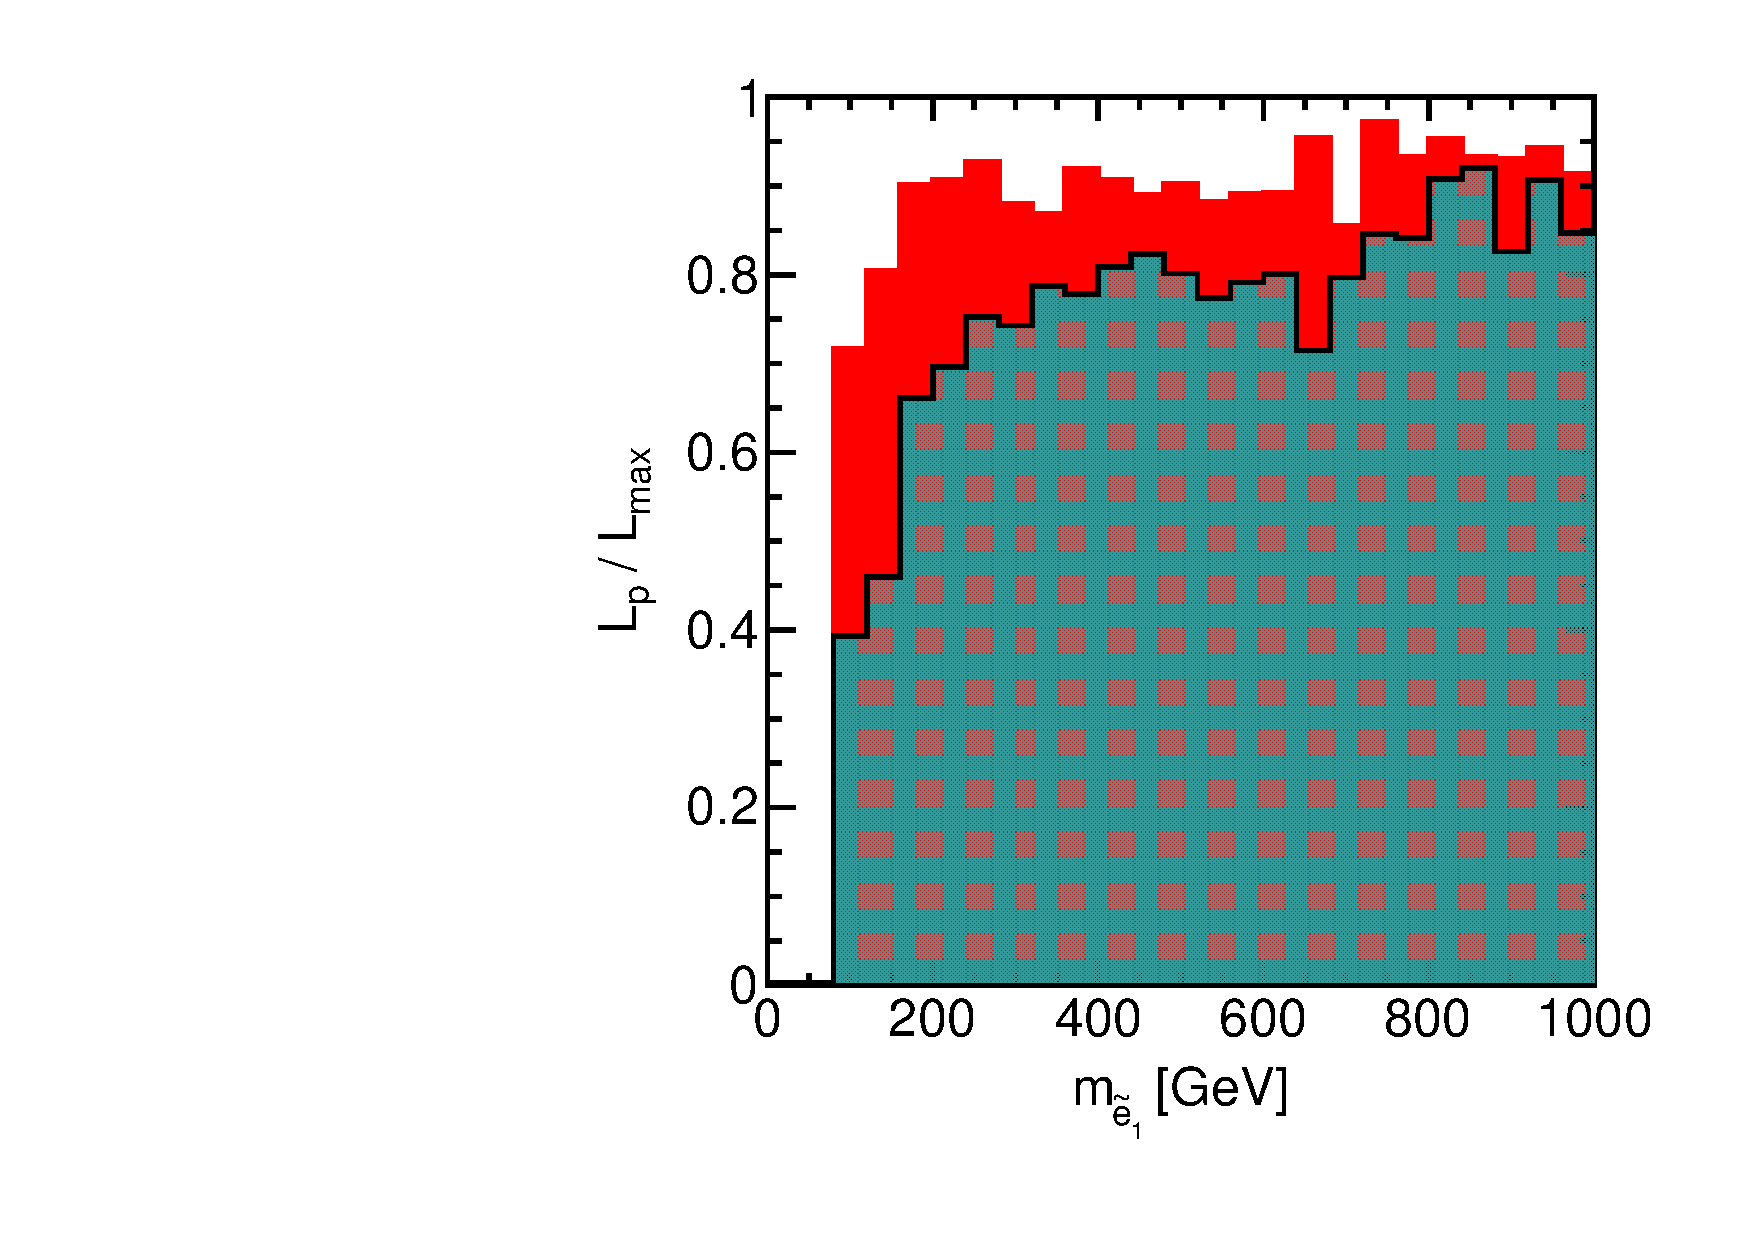
\includegraphics[height=5.5cm]{figs/fig_m_e_1.pdf}
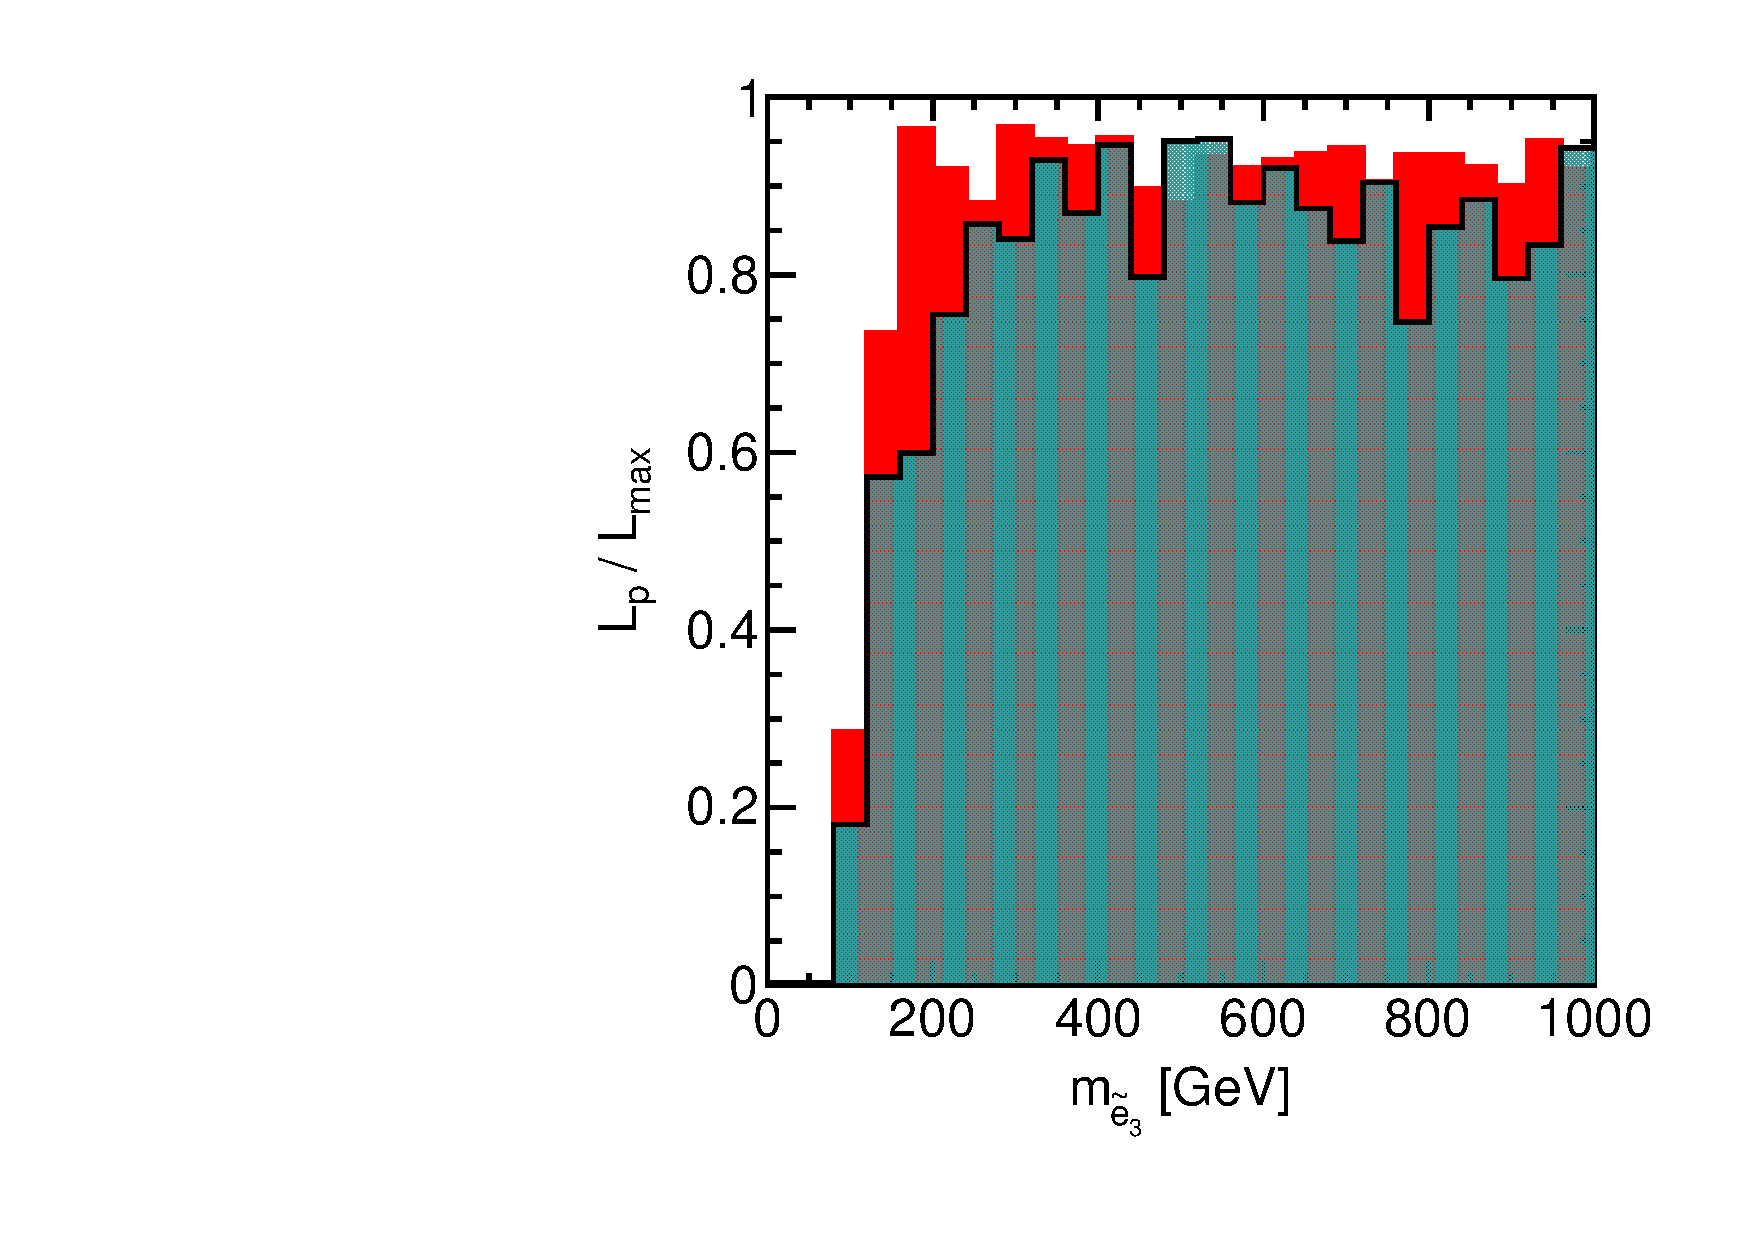
\includegraphics[height=5.5cm]{figs/fig_m_e_3.pdf}
\caption{Slepton mass parameters at the SUSY scale}
\label{default}
\end{center}
\end{figure}


\begin{figure}[htbp]
\begin{center}
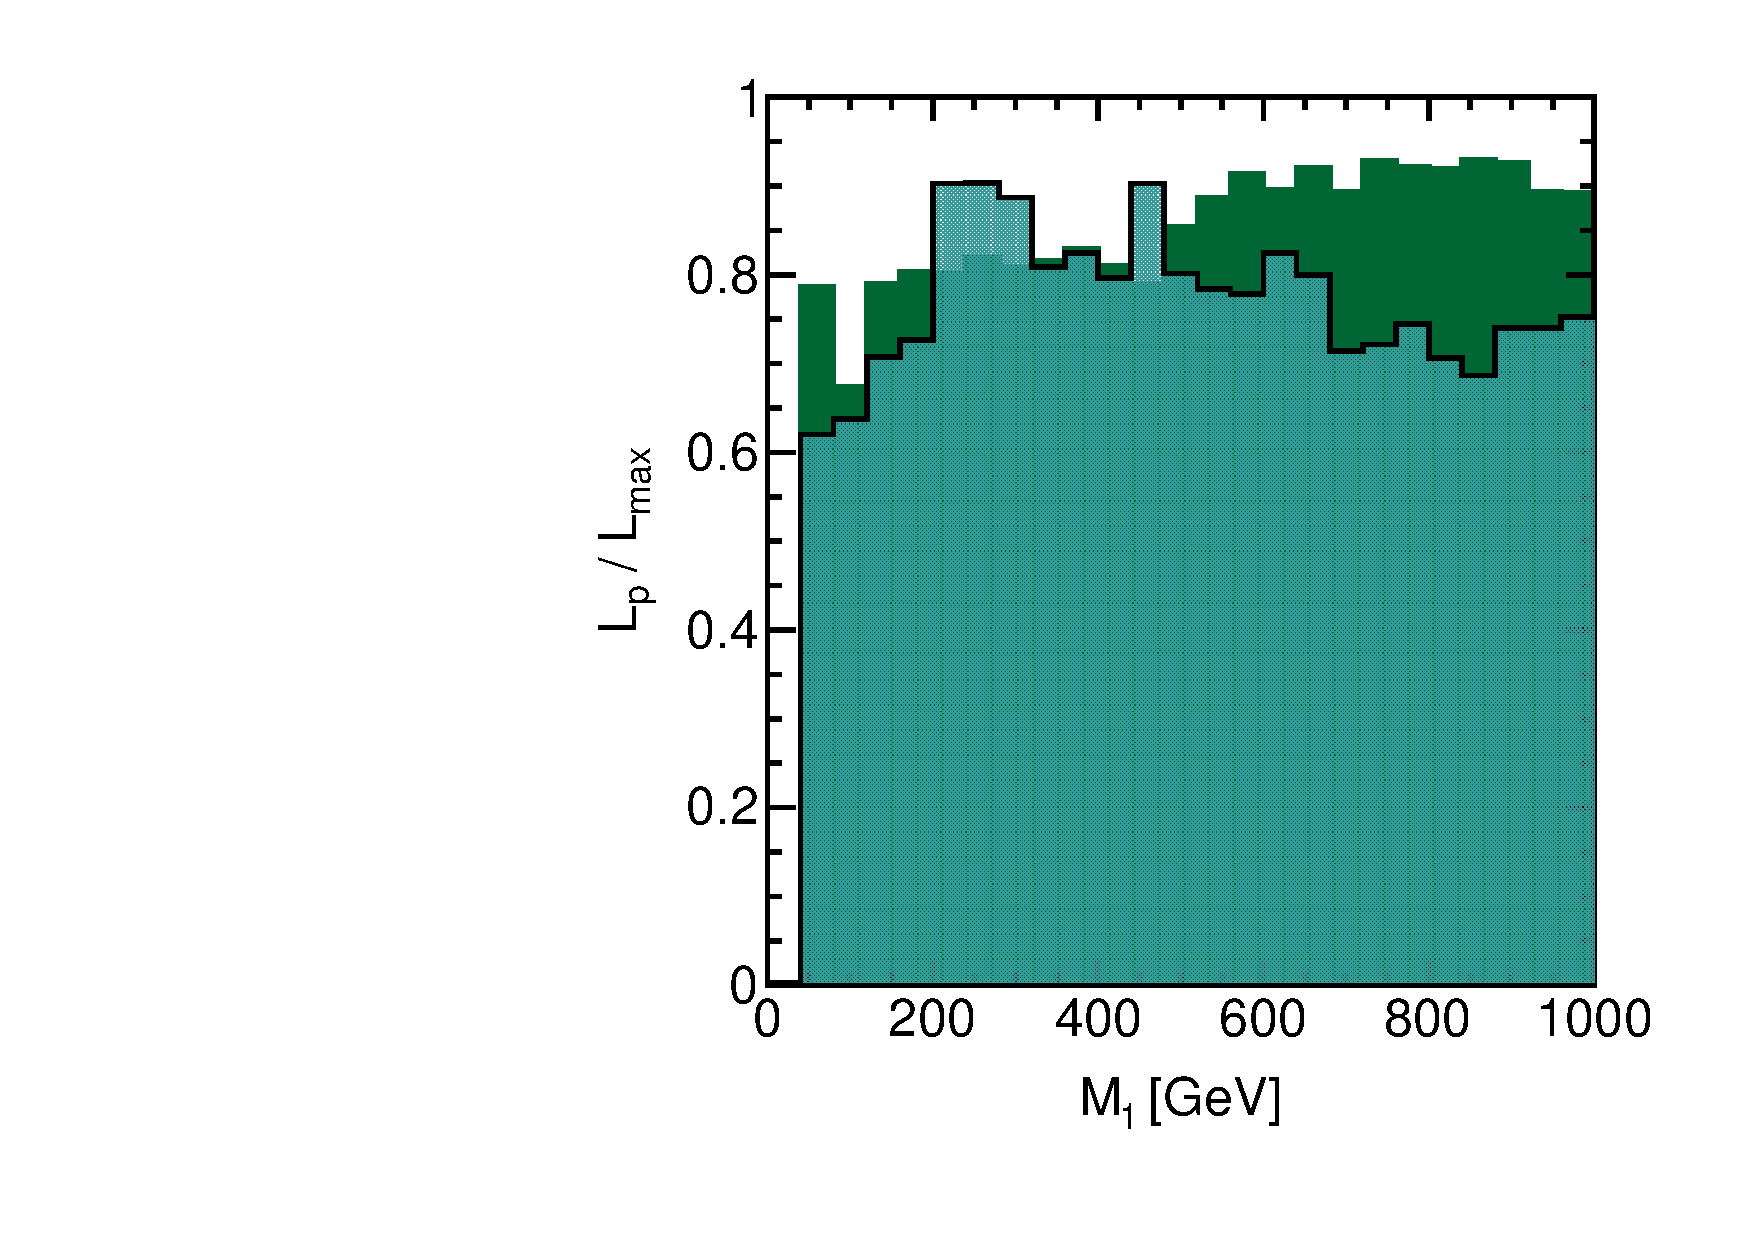
\includegraphics[height=5.5cm]{figs/fig_M_1.pdf} 
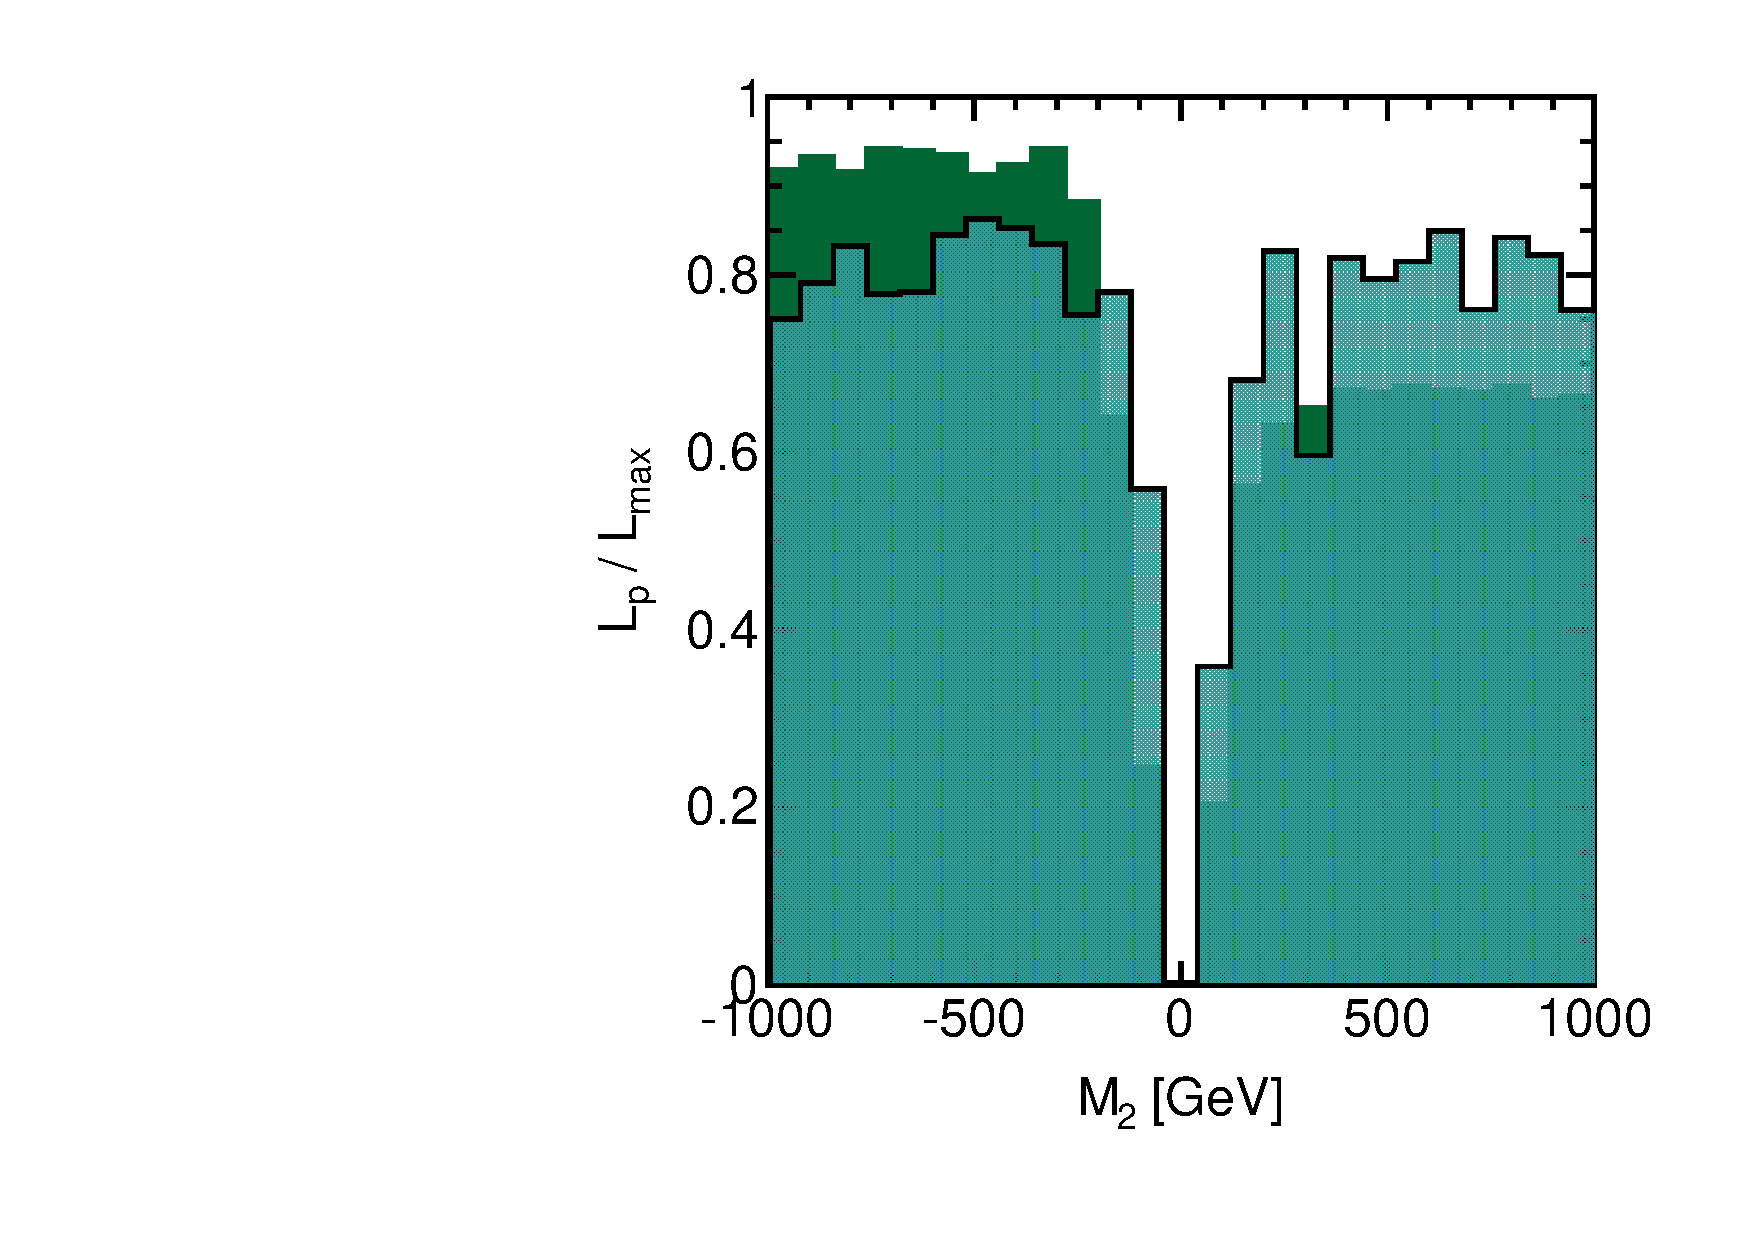
\includegraphics[height=5.5cm]{figs/fig_M_2.pdf} \\
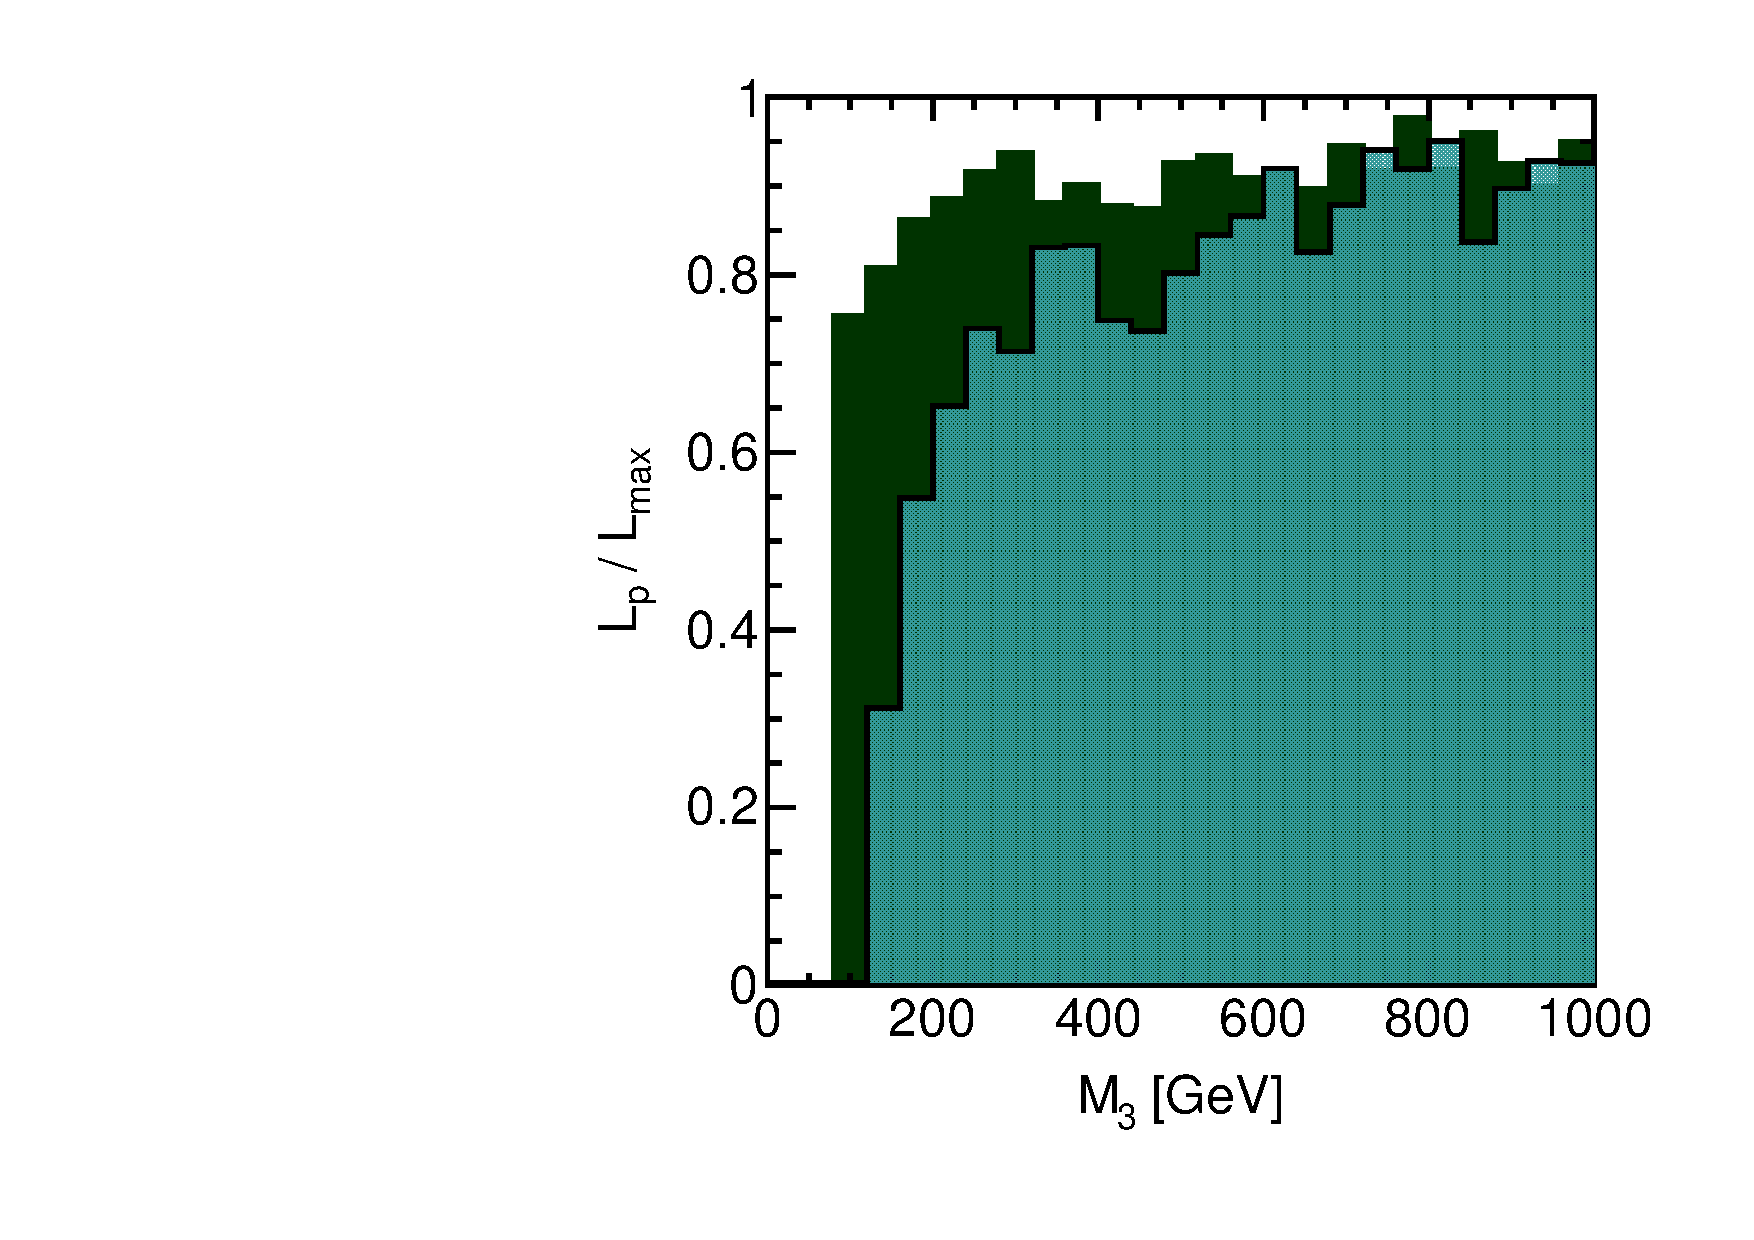
\includegraphics[height=5.5cm]{figs/fig_M_3.pdf}
\caption{Gaugino mass parameters at the SUSY scale.}
\label{default}
\end{center}
\end{figure}


\begin{figure}[htbp]
\begin{center}
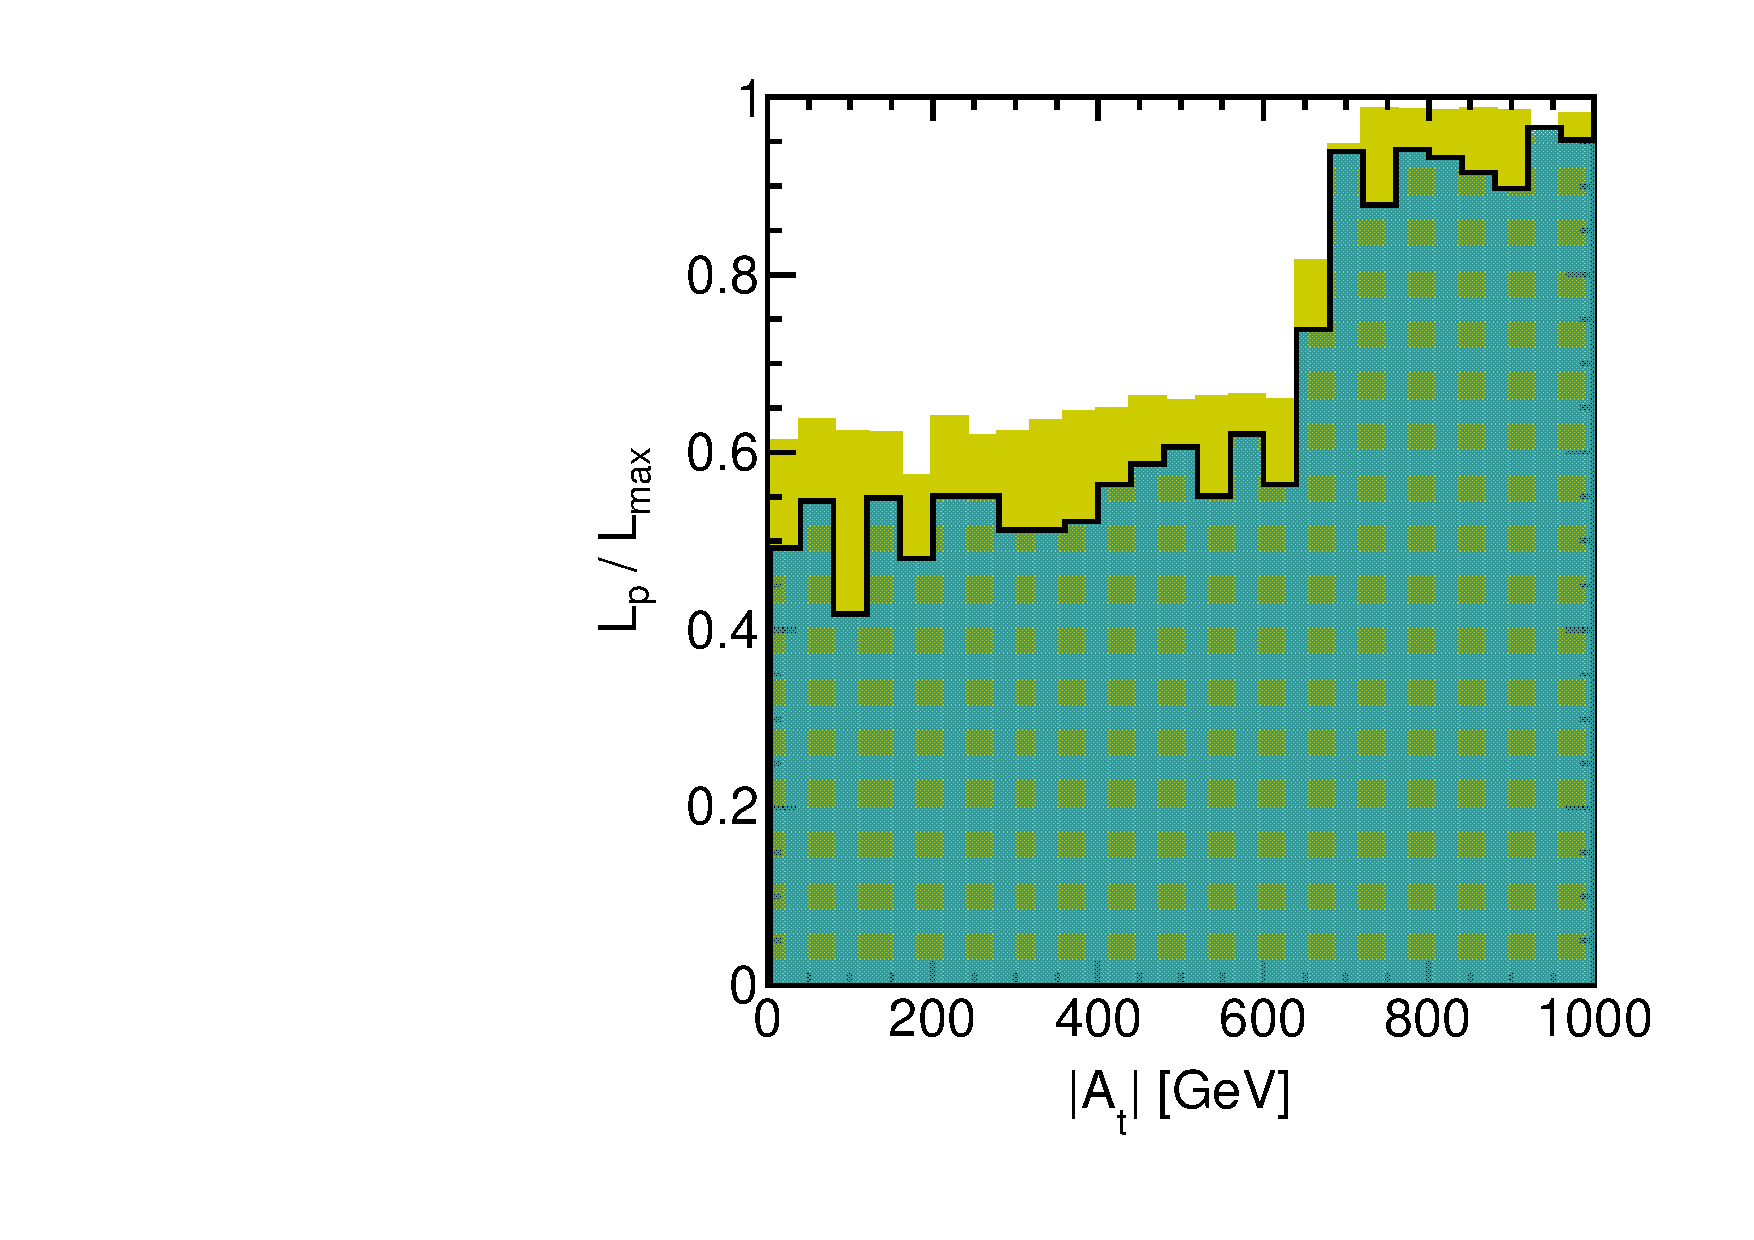
\includegraphics[height=5.5cm]{figs/fig_A_t.pdf} 
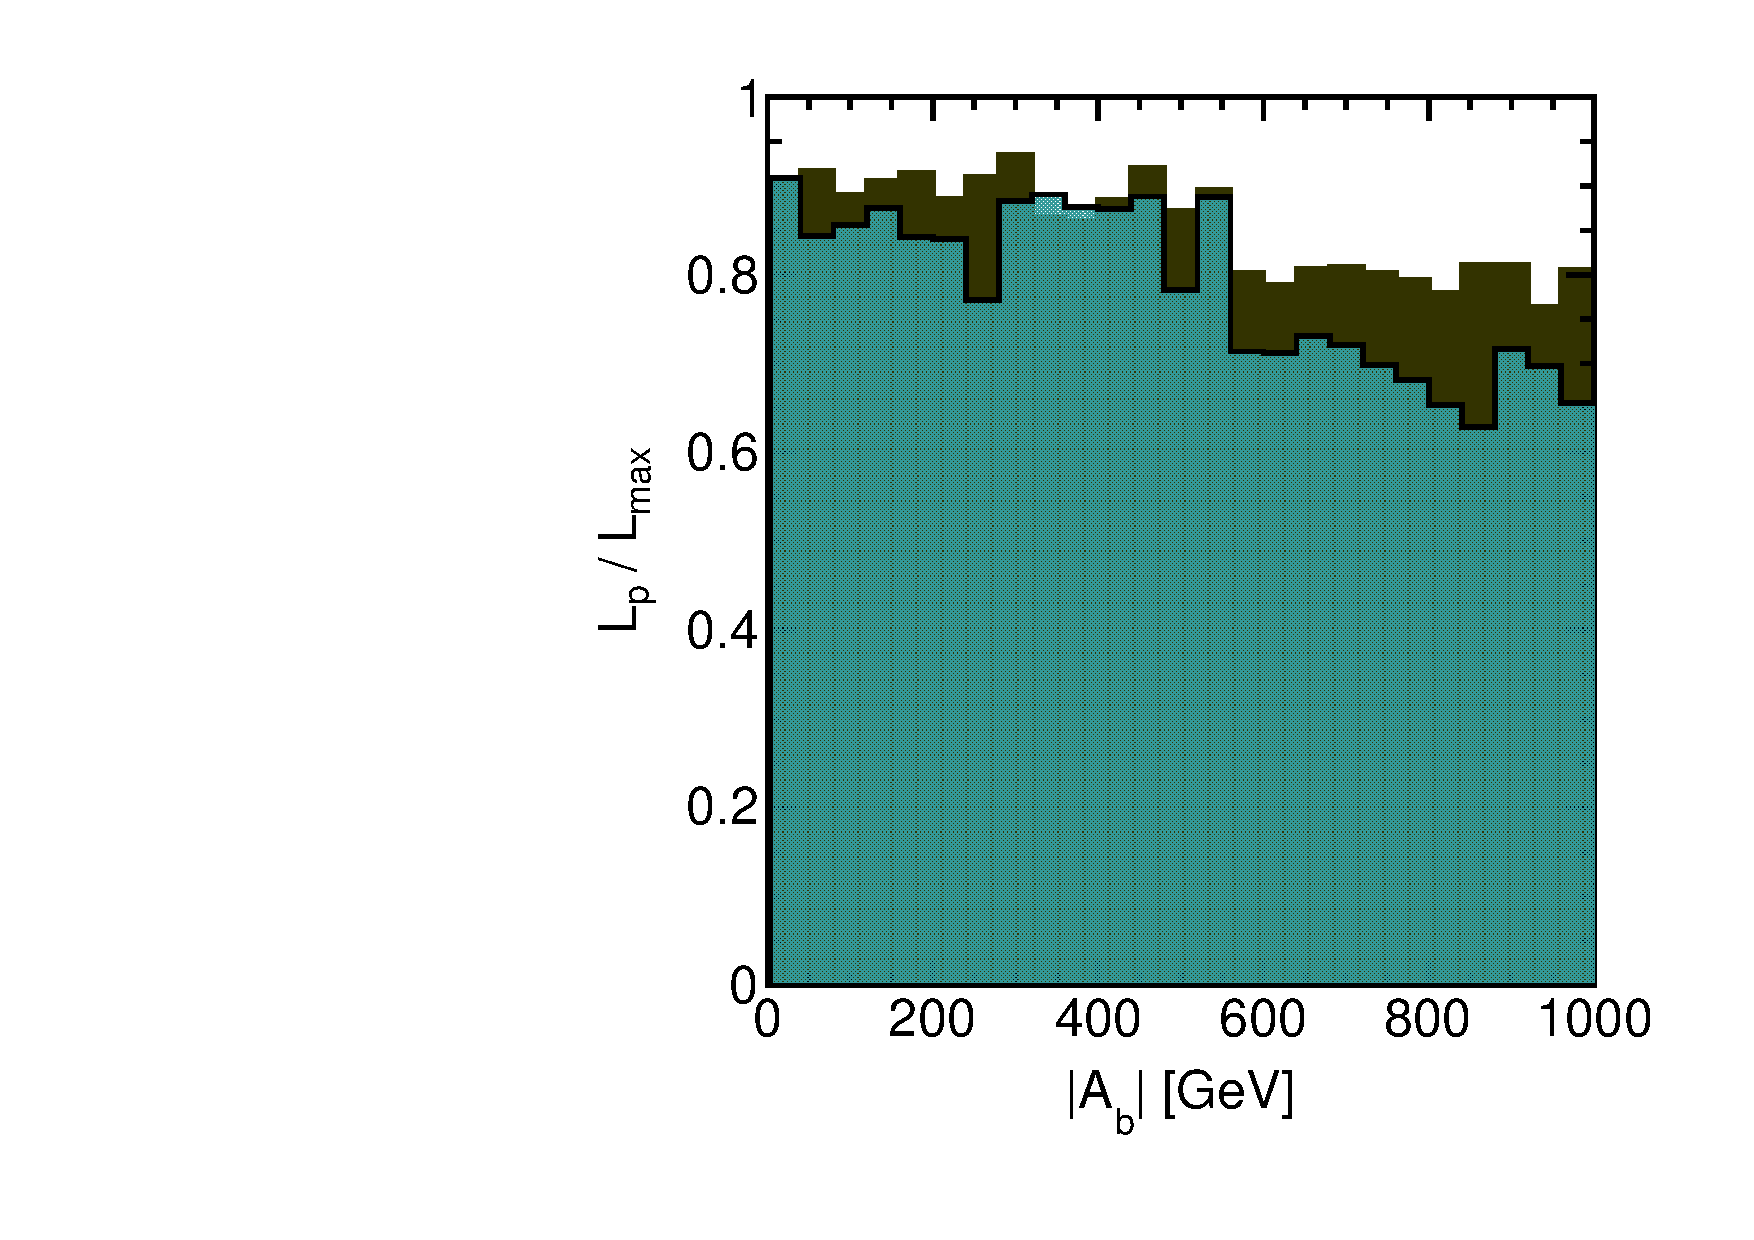
\includegraphics[height=5.5cm]{figs/fig_A_b.pdf} \\
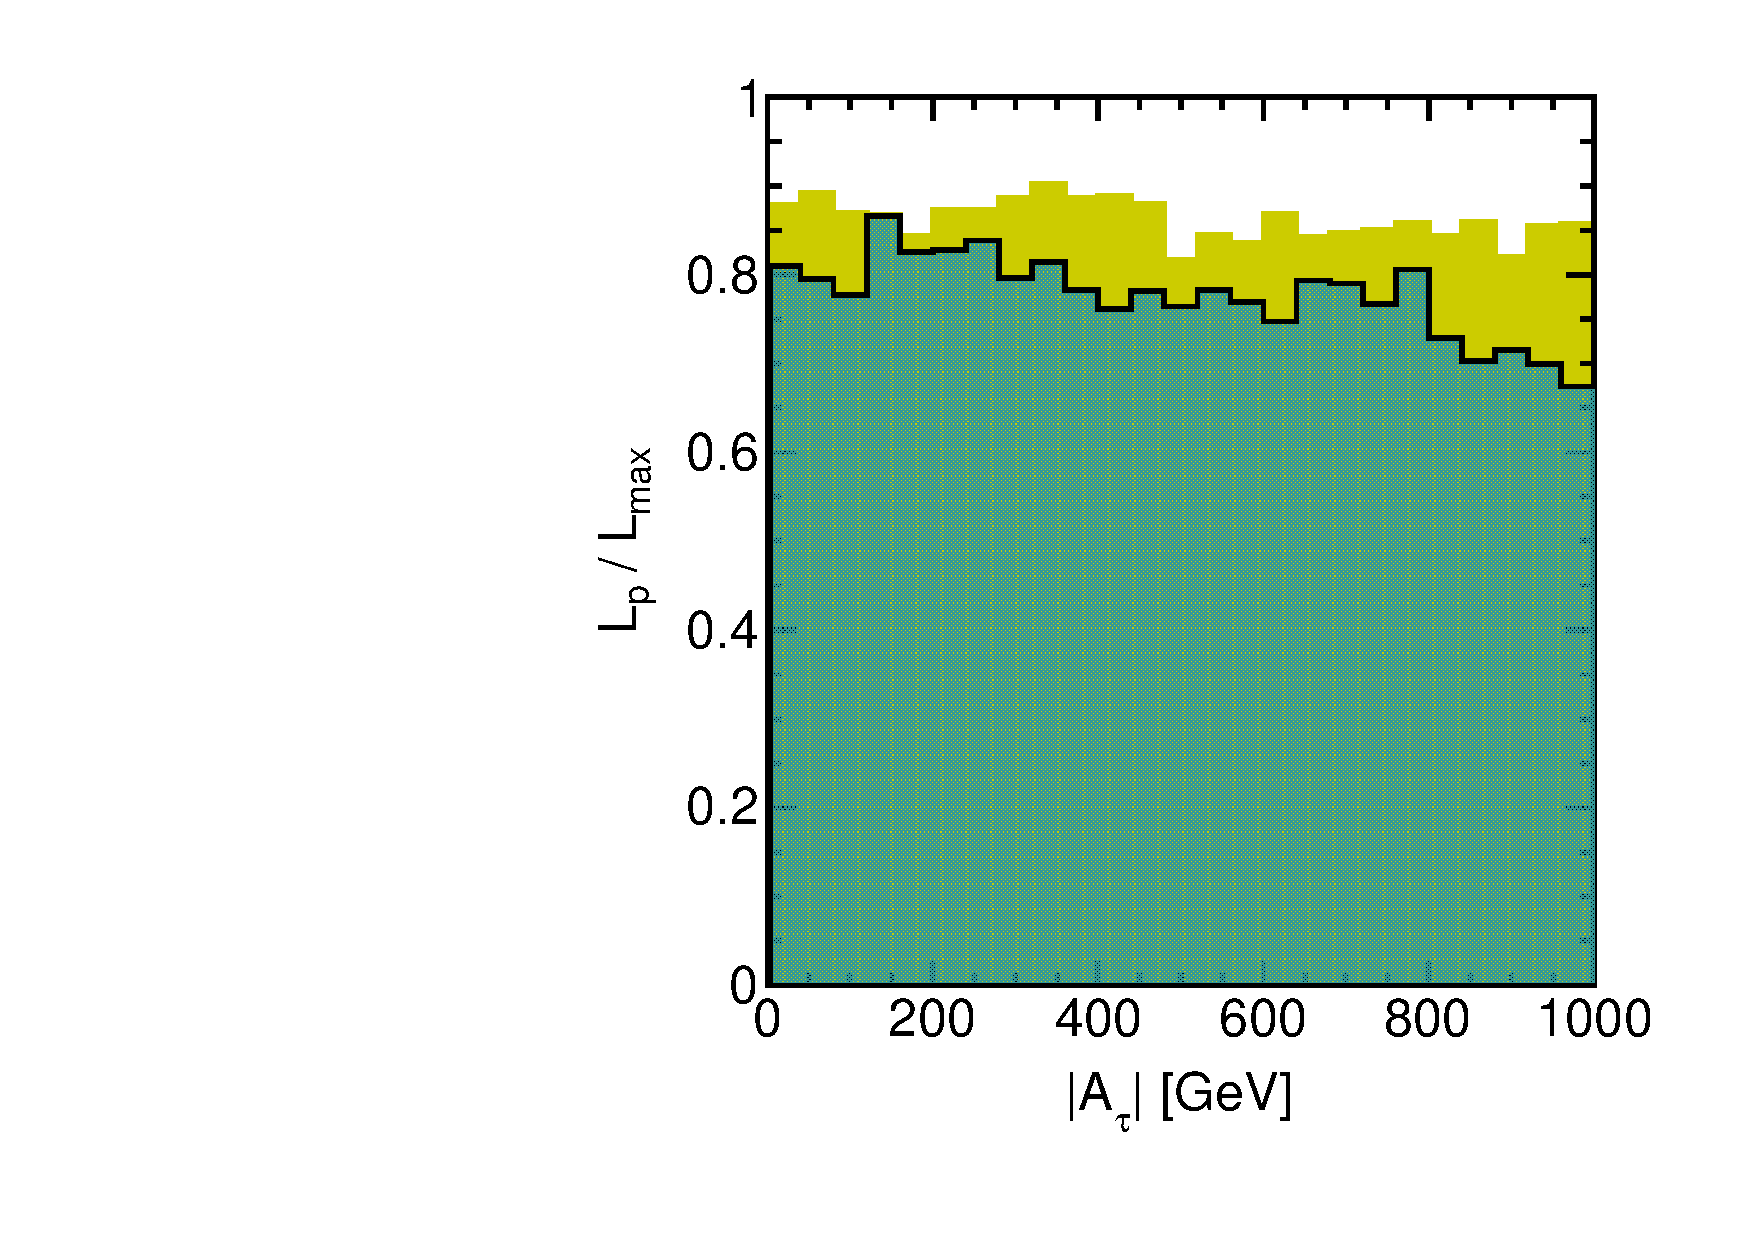
\includegraphics[height=5.5cm]{figs/fig_A_tau.pdf}
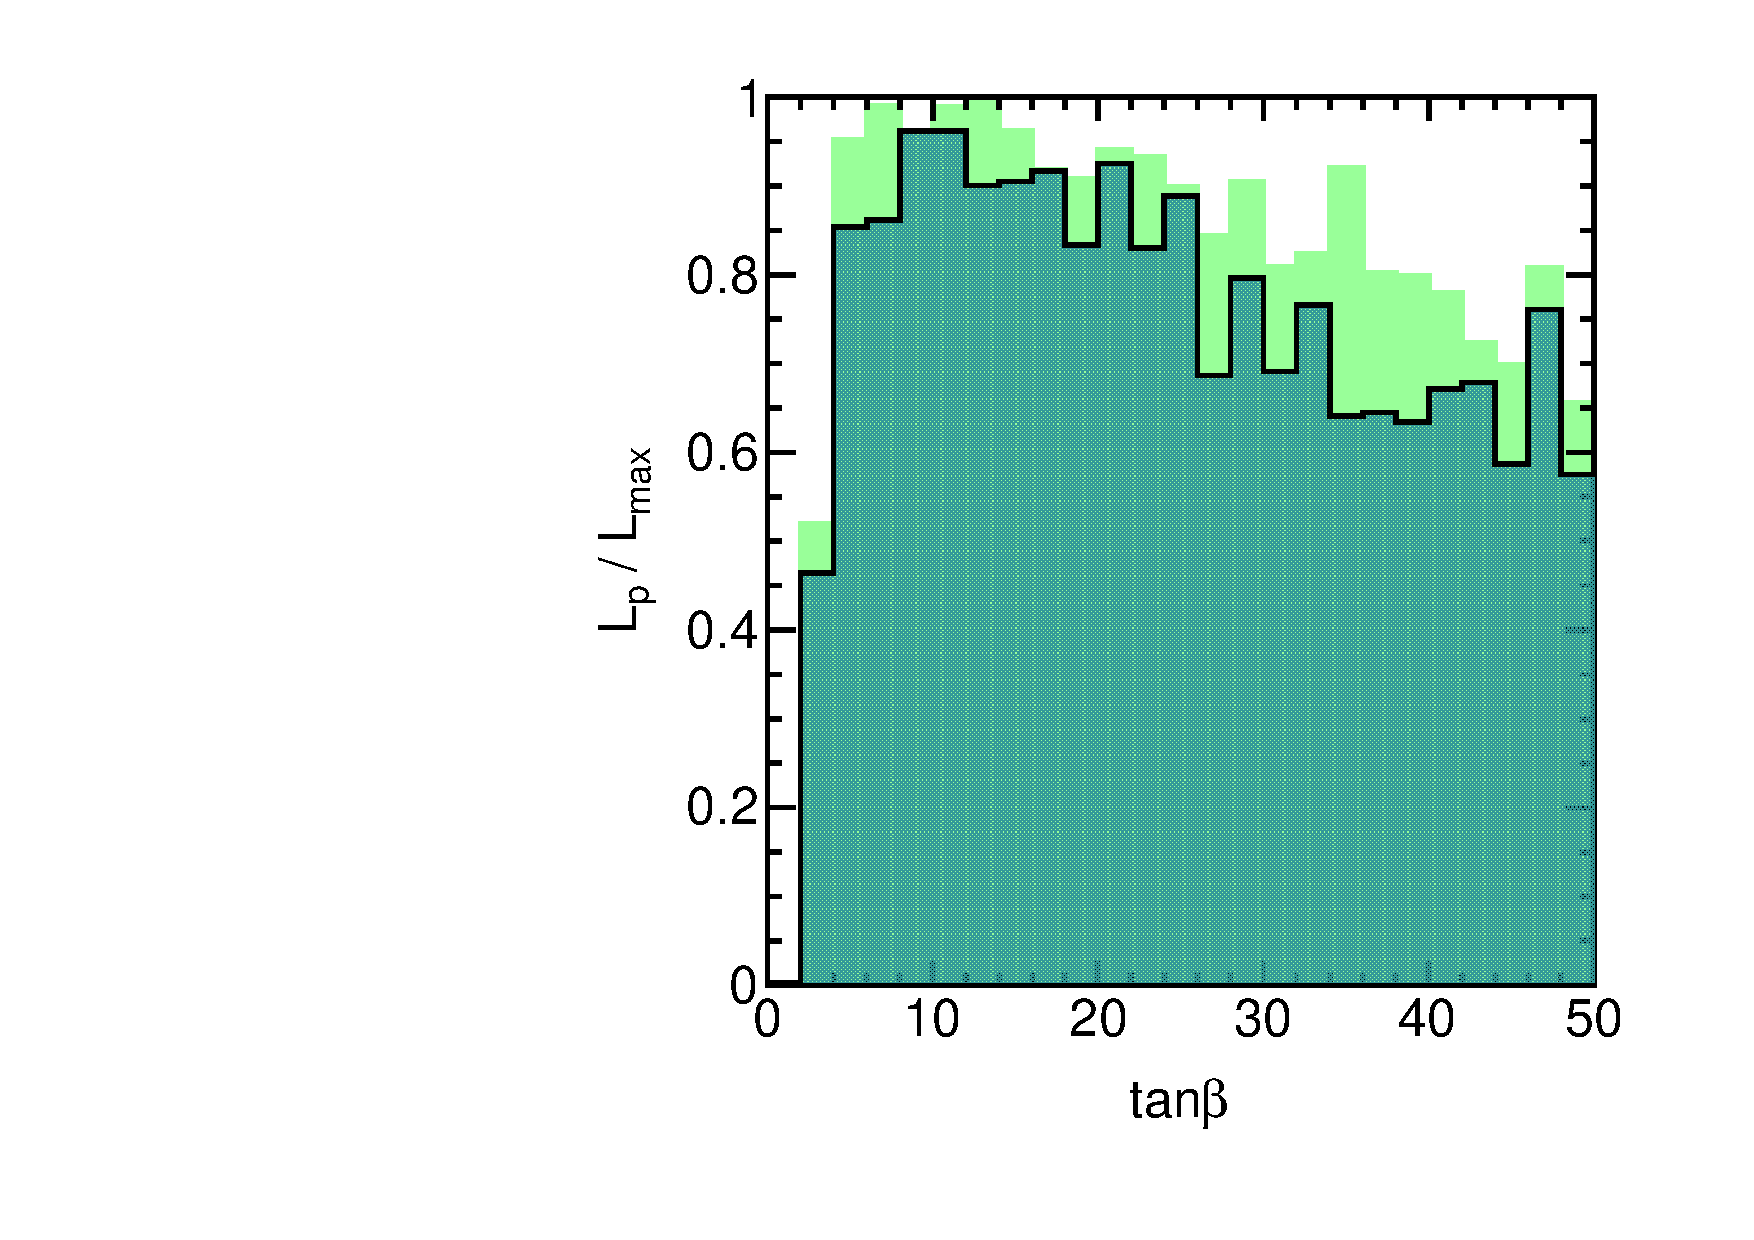
\includegraphics[height=5.5cm]{figs/fig_tanbeta.pdf}
\caption{Trilinear couplings and $\tan\beta$ at the SUSY scale}
\label{default}
\end{center}
\end{figure}


\begin{figure}[htbp]
\begin{center}
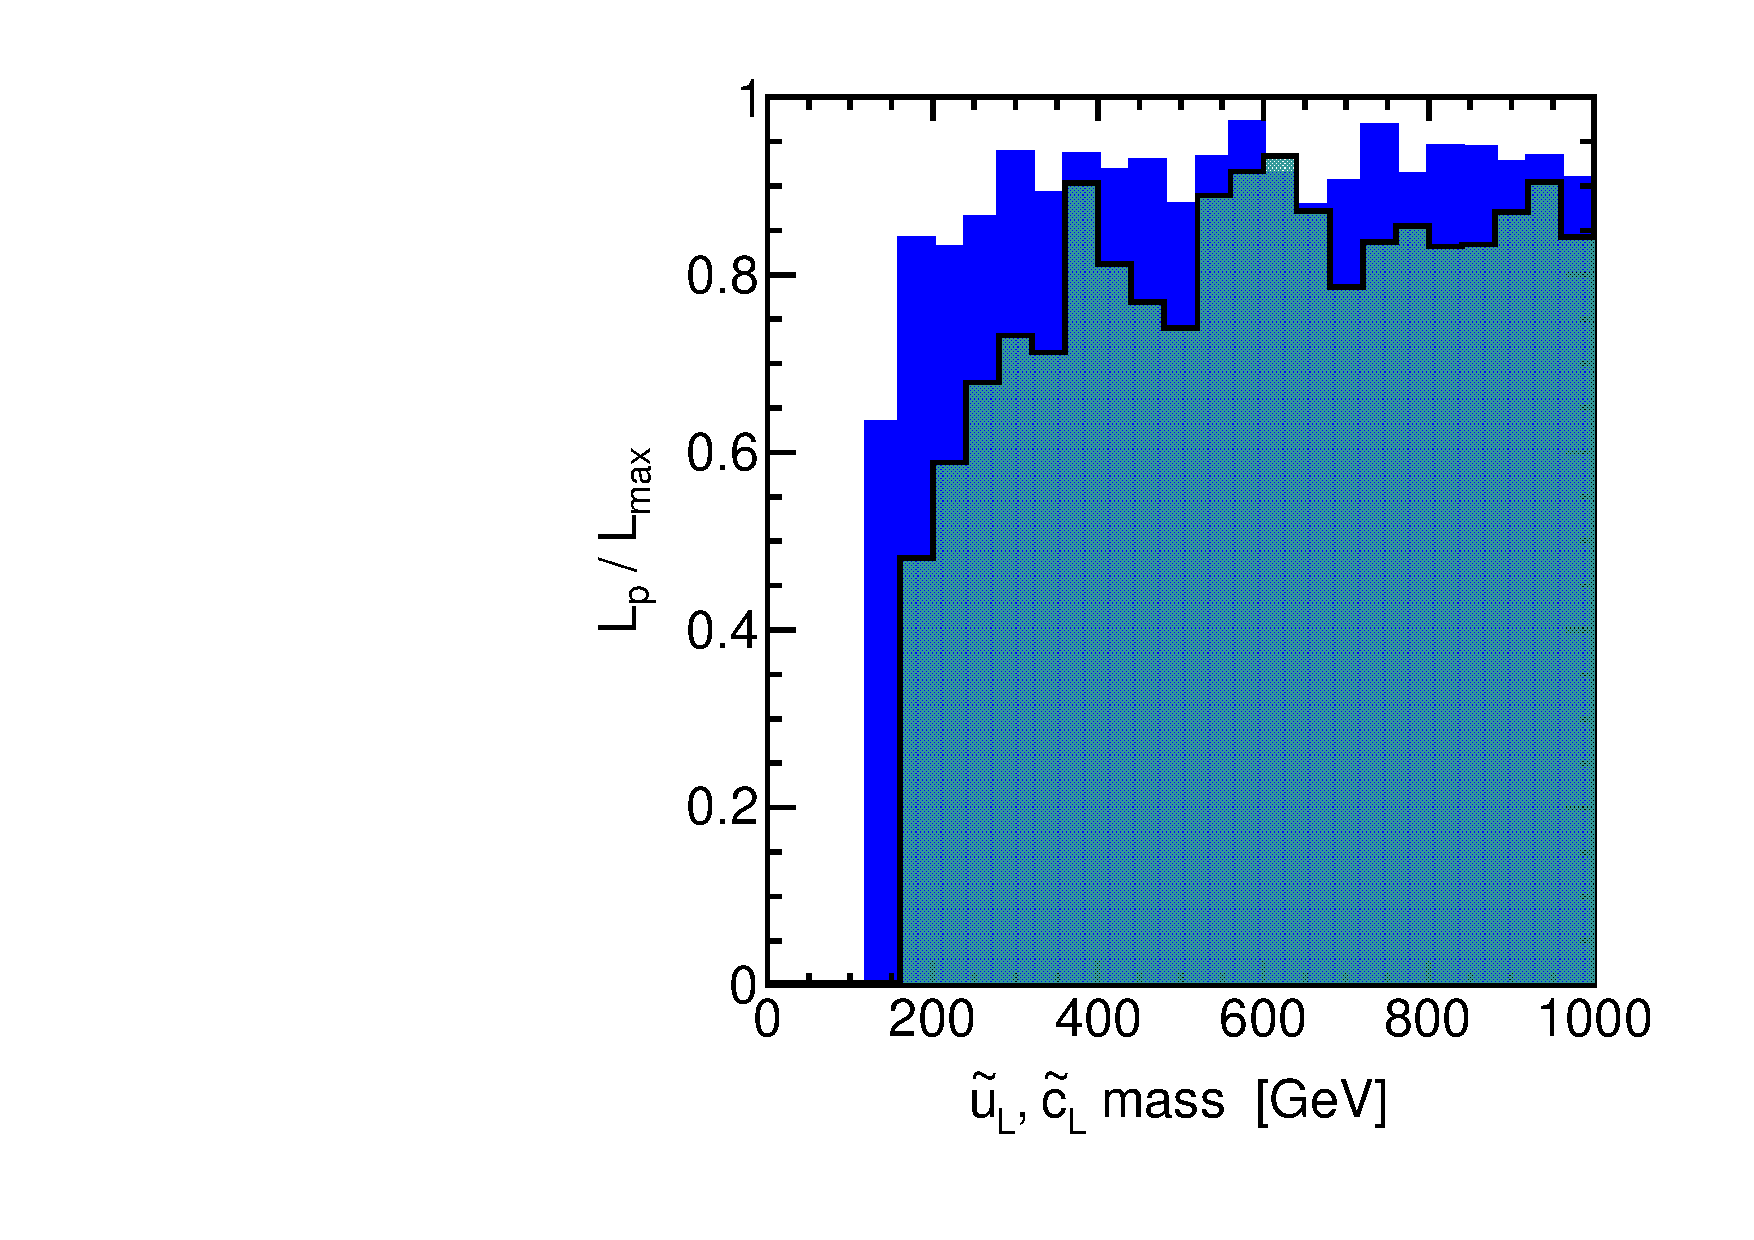
\includegraphics[height=5.5cm]{figs/fig_u_L.pdf} 
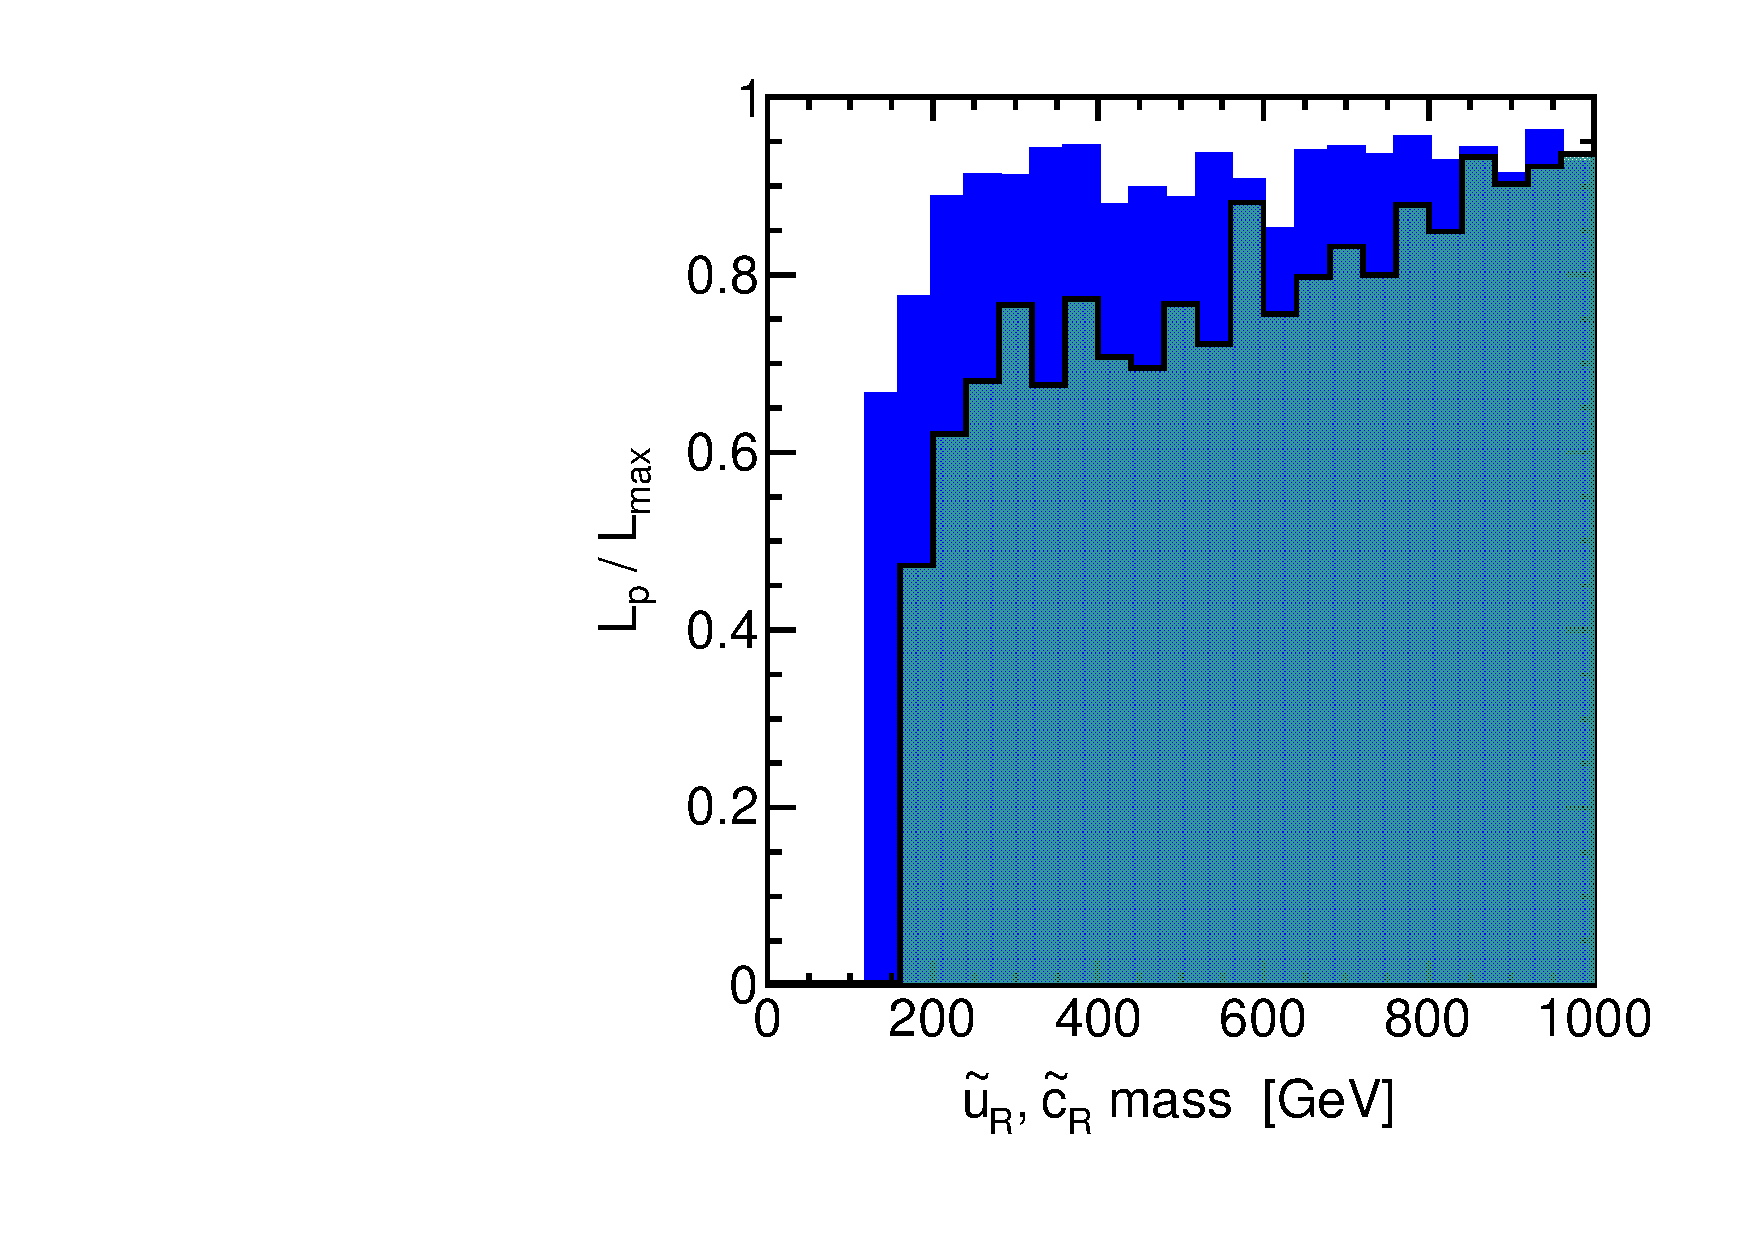
\includegraphics[height=5.5cm]{figs/fig_u_R.pdf} \\
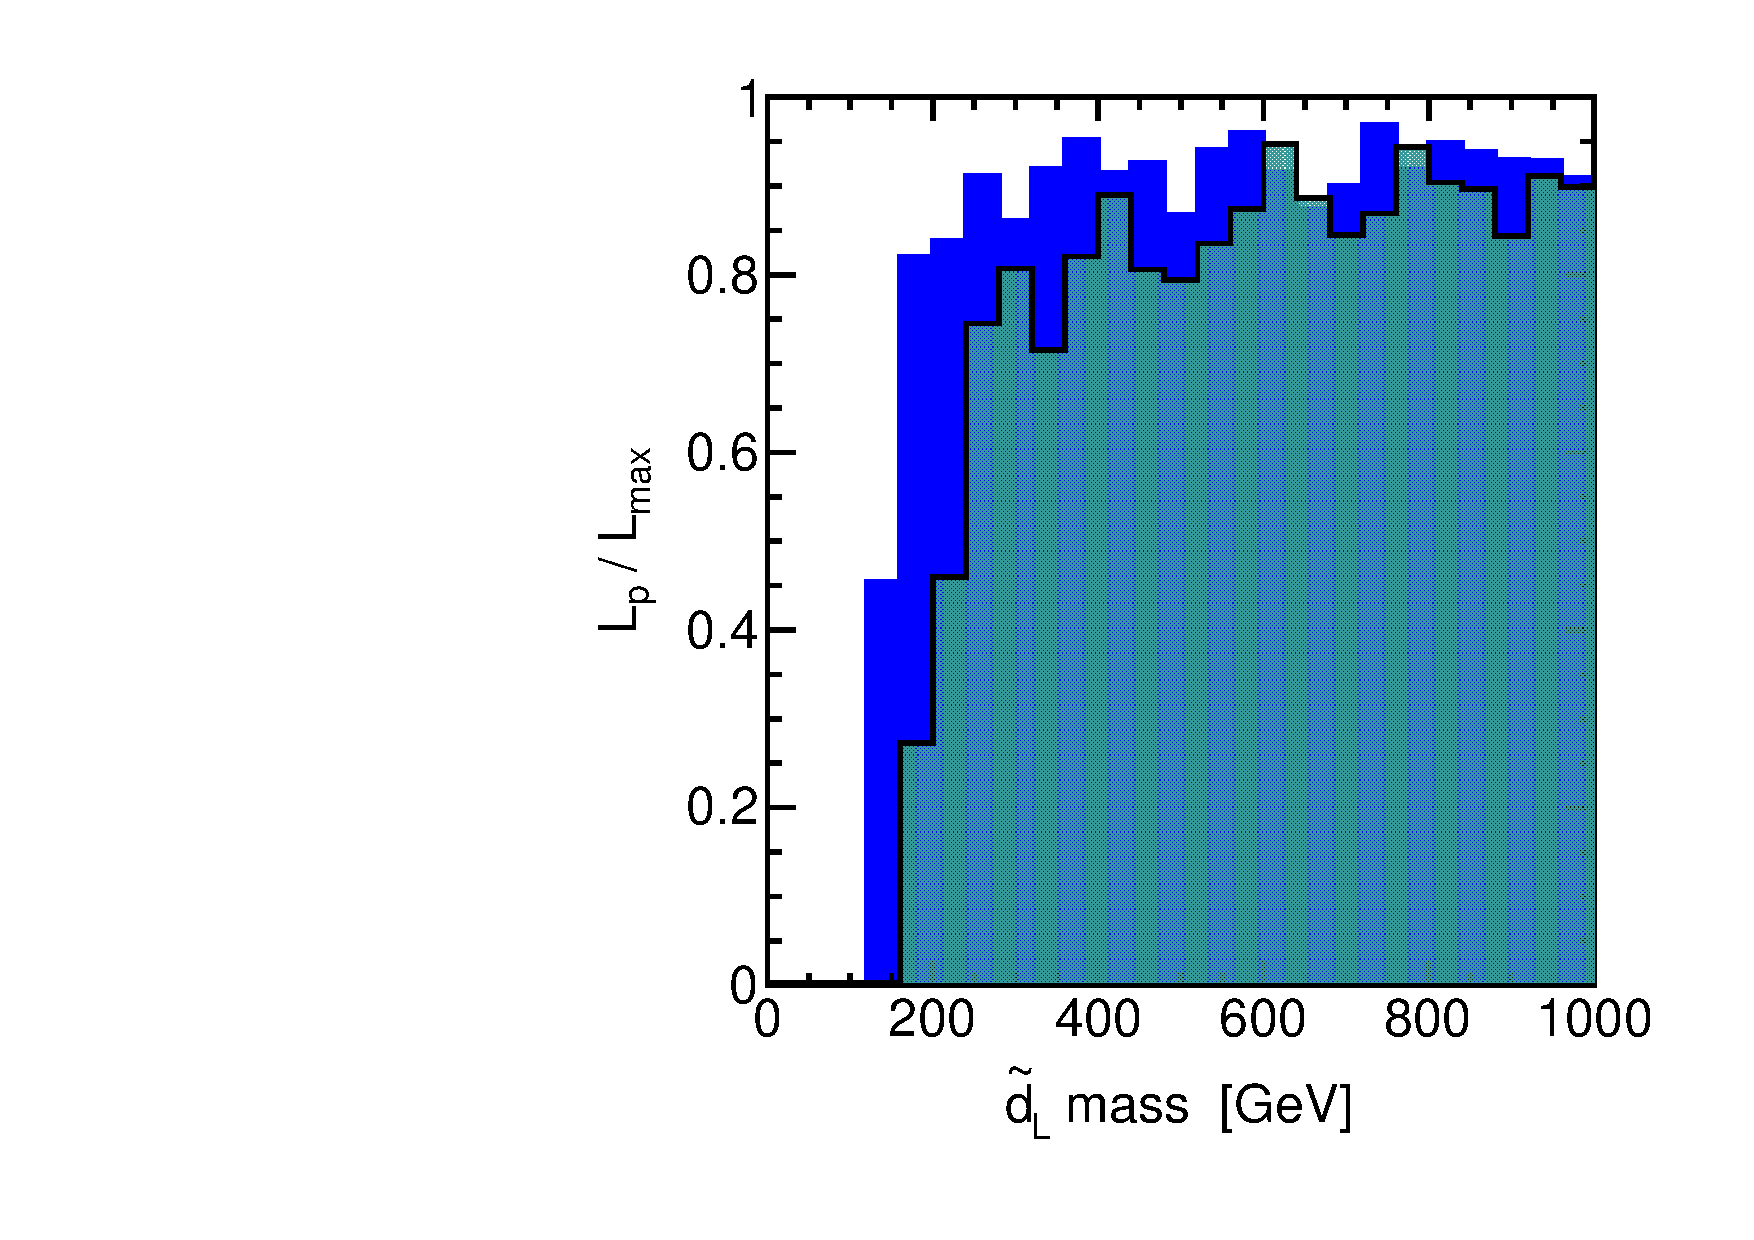
\includegraphics[height=5.5cm]{figs/fig_d_L.pdf} 
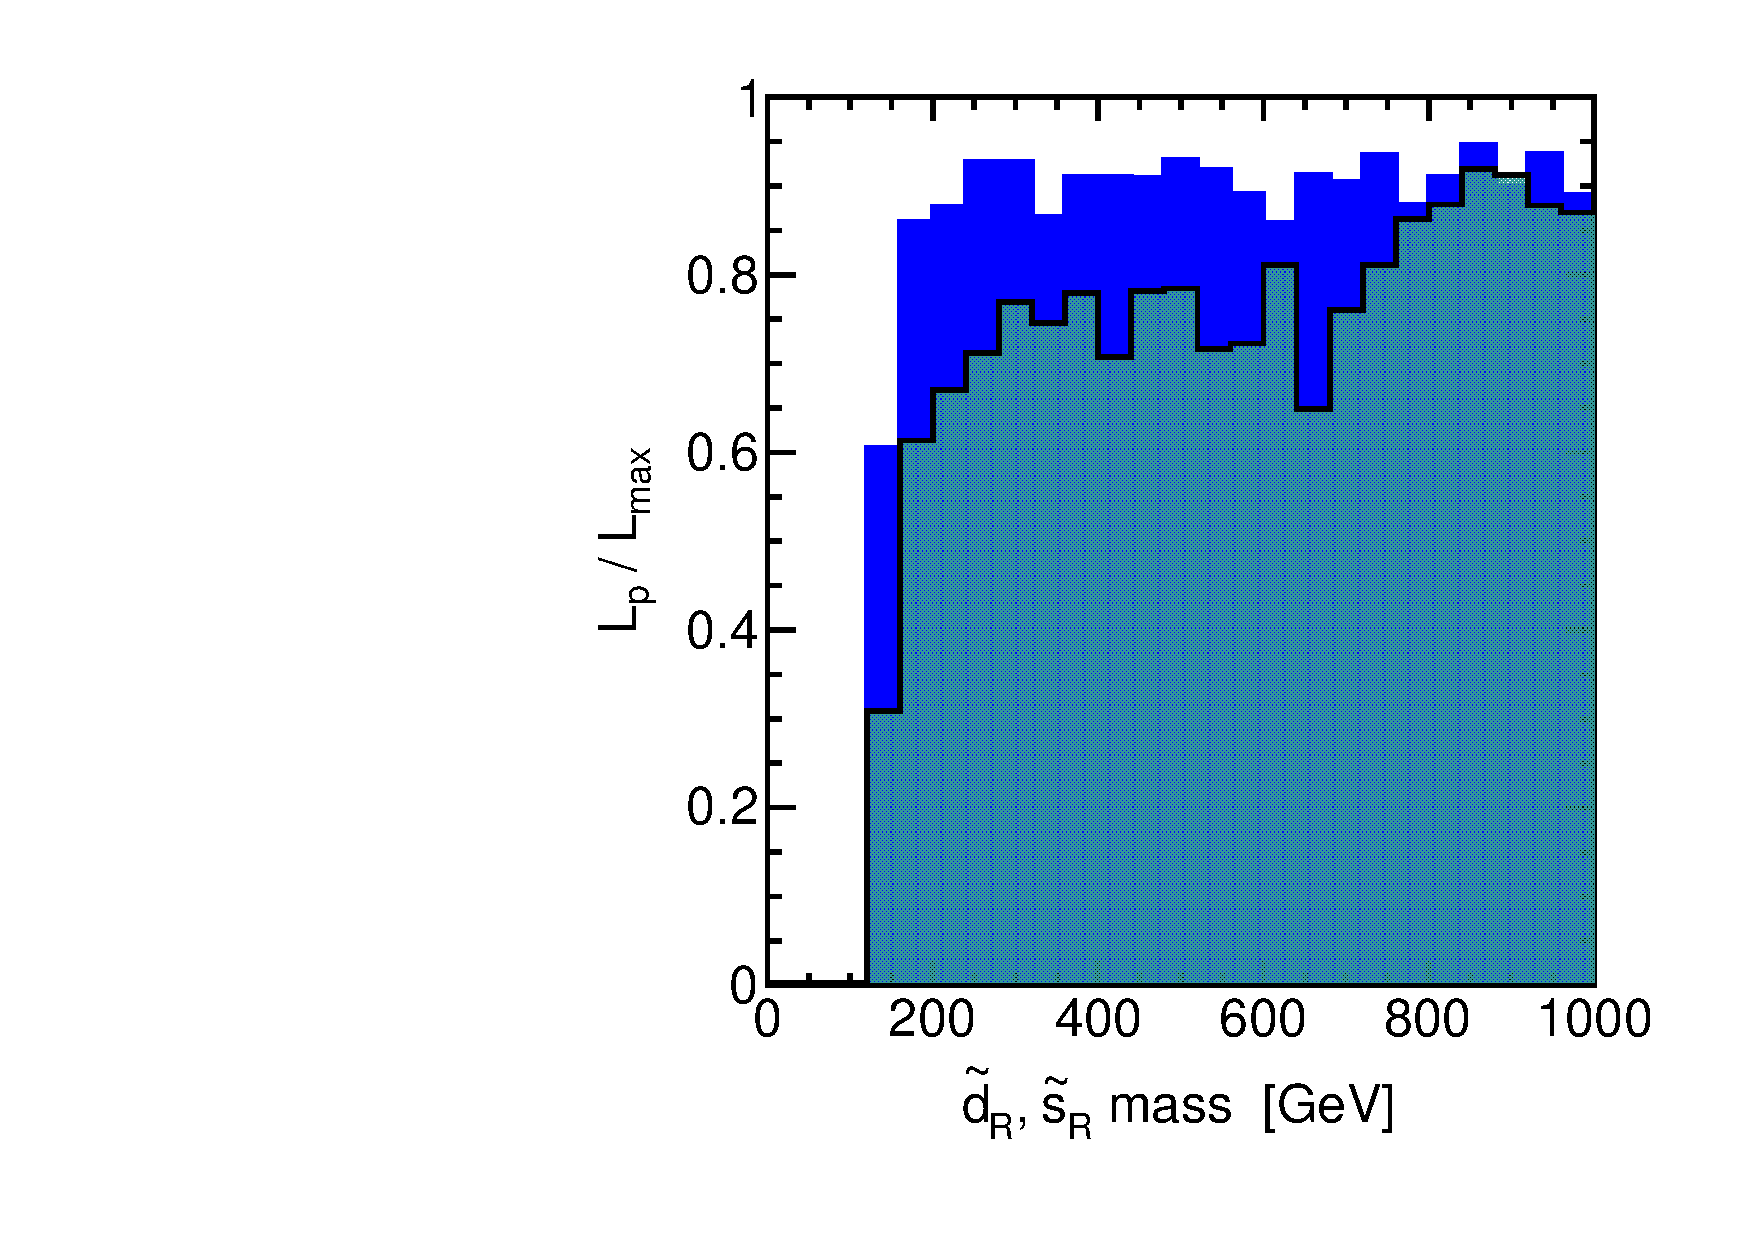
\includegraphics[height=5.5cm]{figs/fig_d_R.pdf} \\
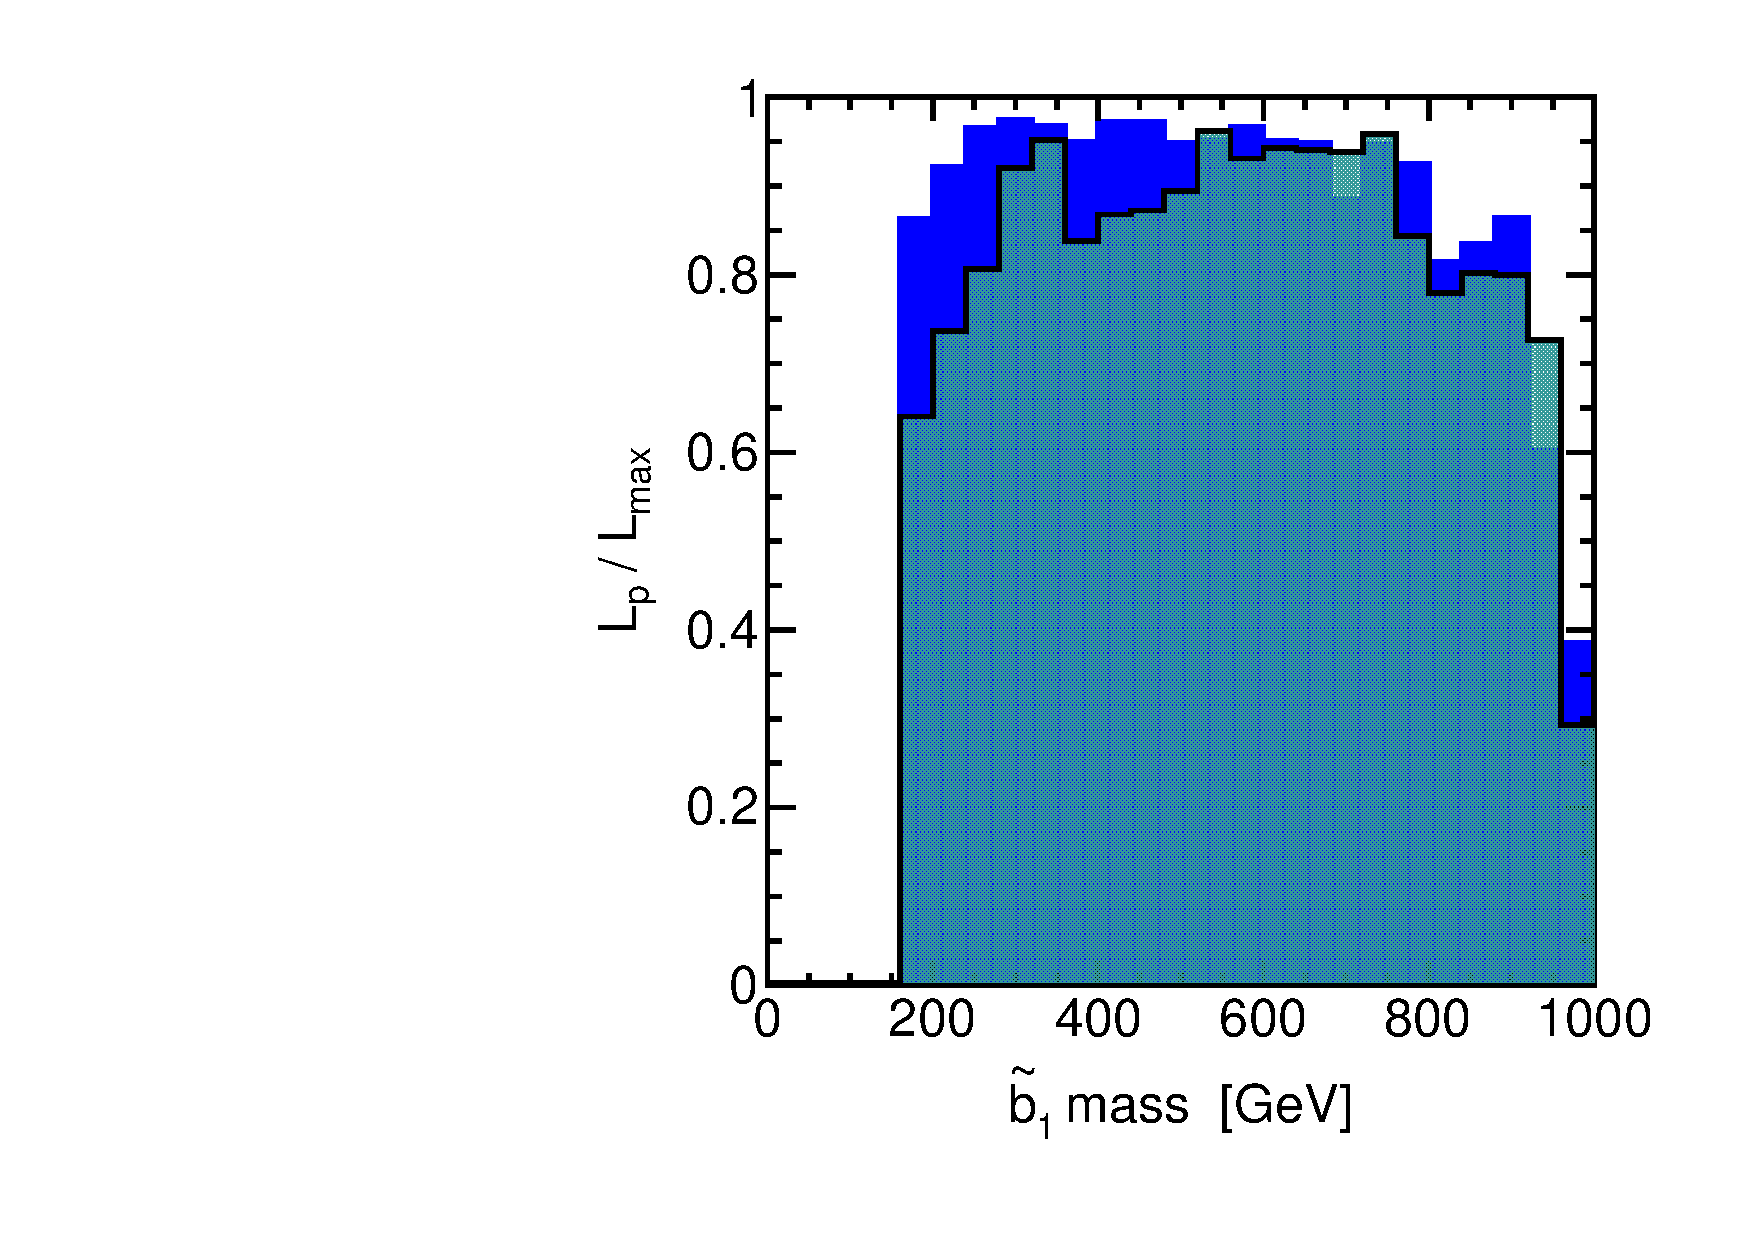
\includegraphics[height=5.5cm]{figs/fig_b_1.pdf} 
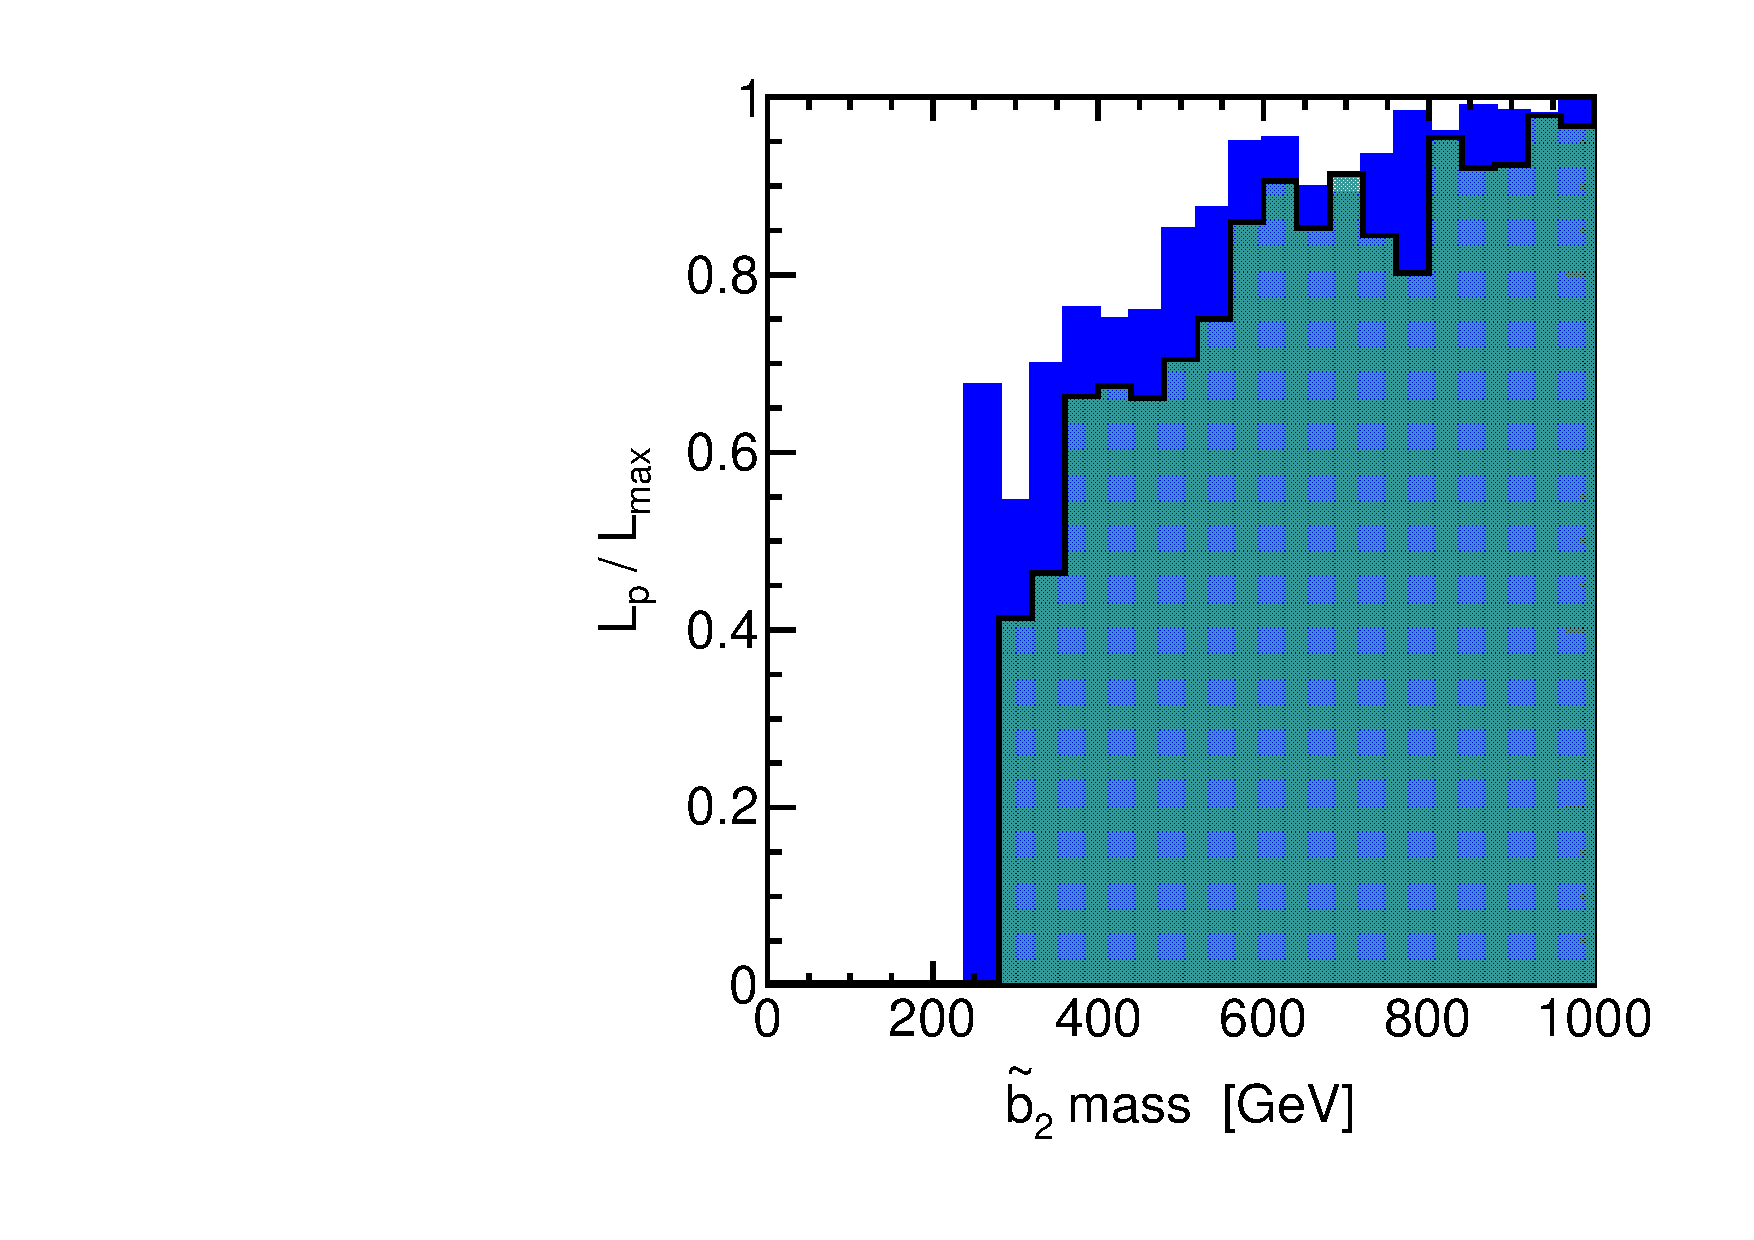
\includegraphics[height=5.5cm]{figs/fig_b_2.pdf} \\
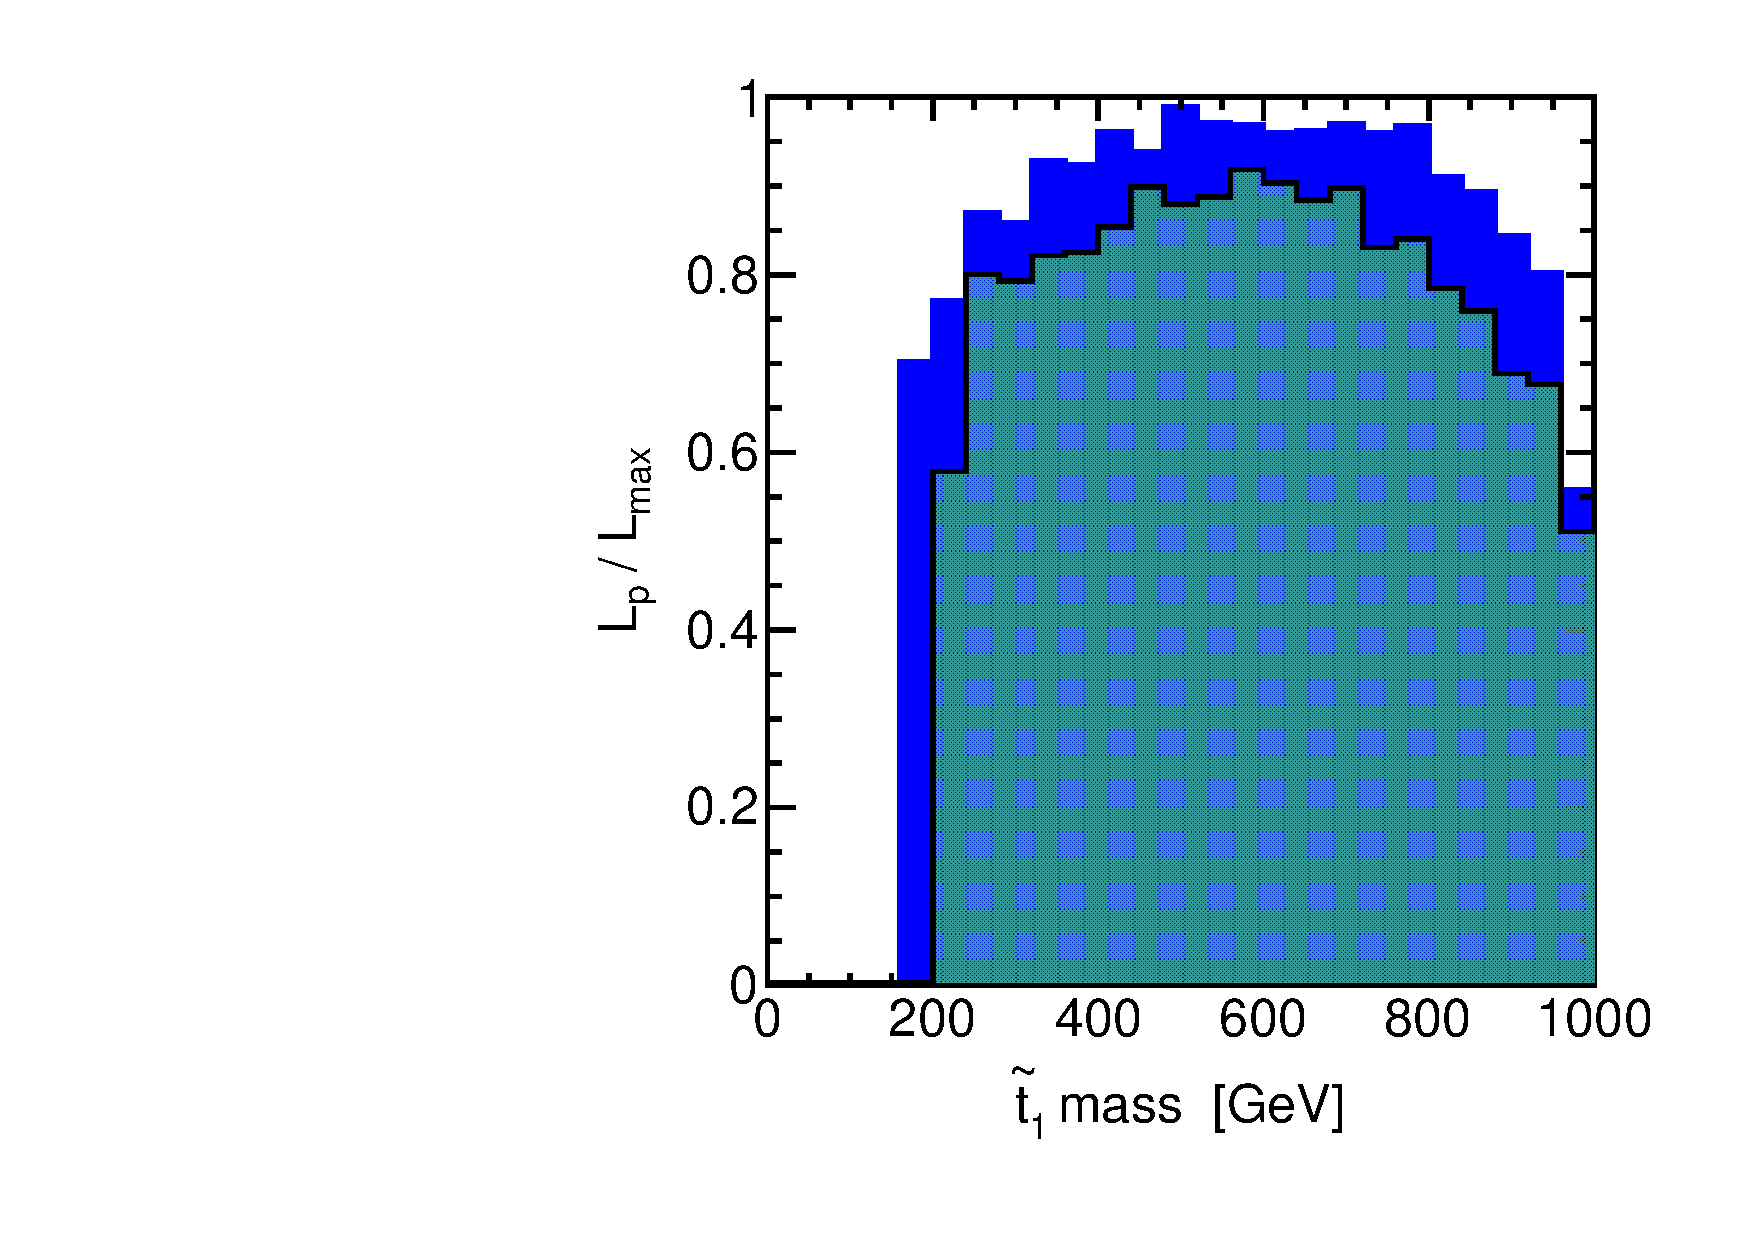
\includegraphics[height=5.5cm]{figs/fig_t_1.pdf} 
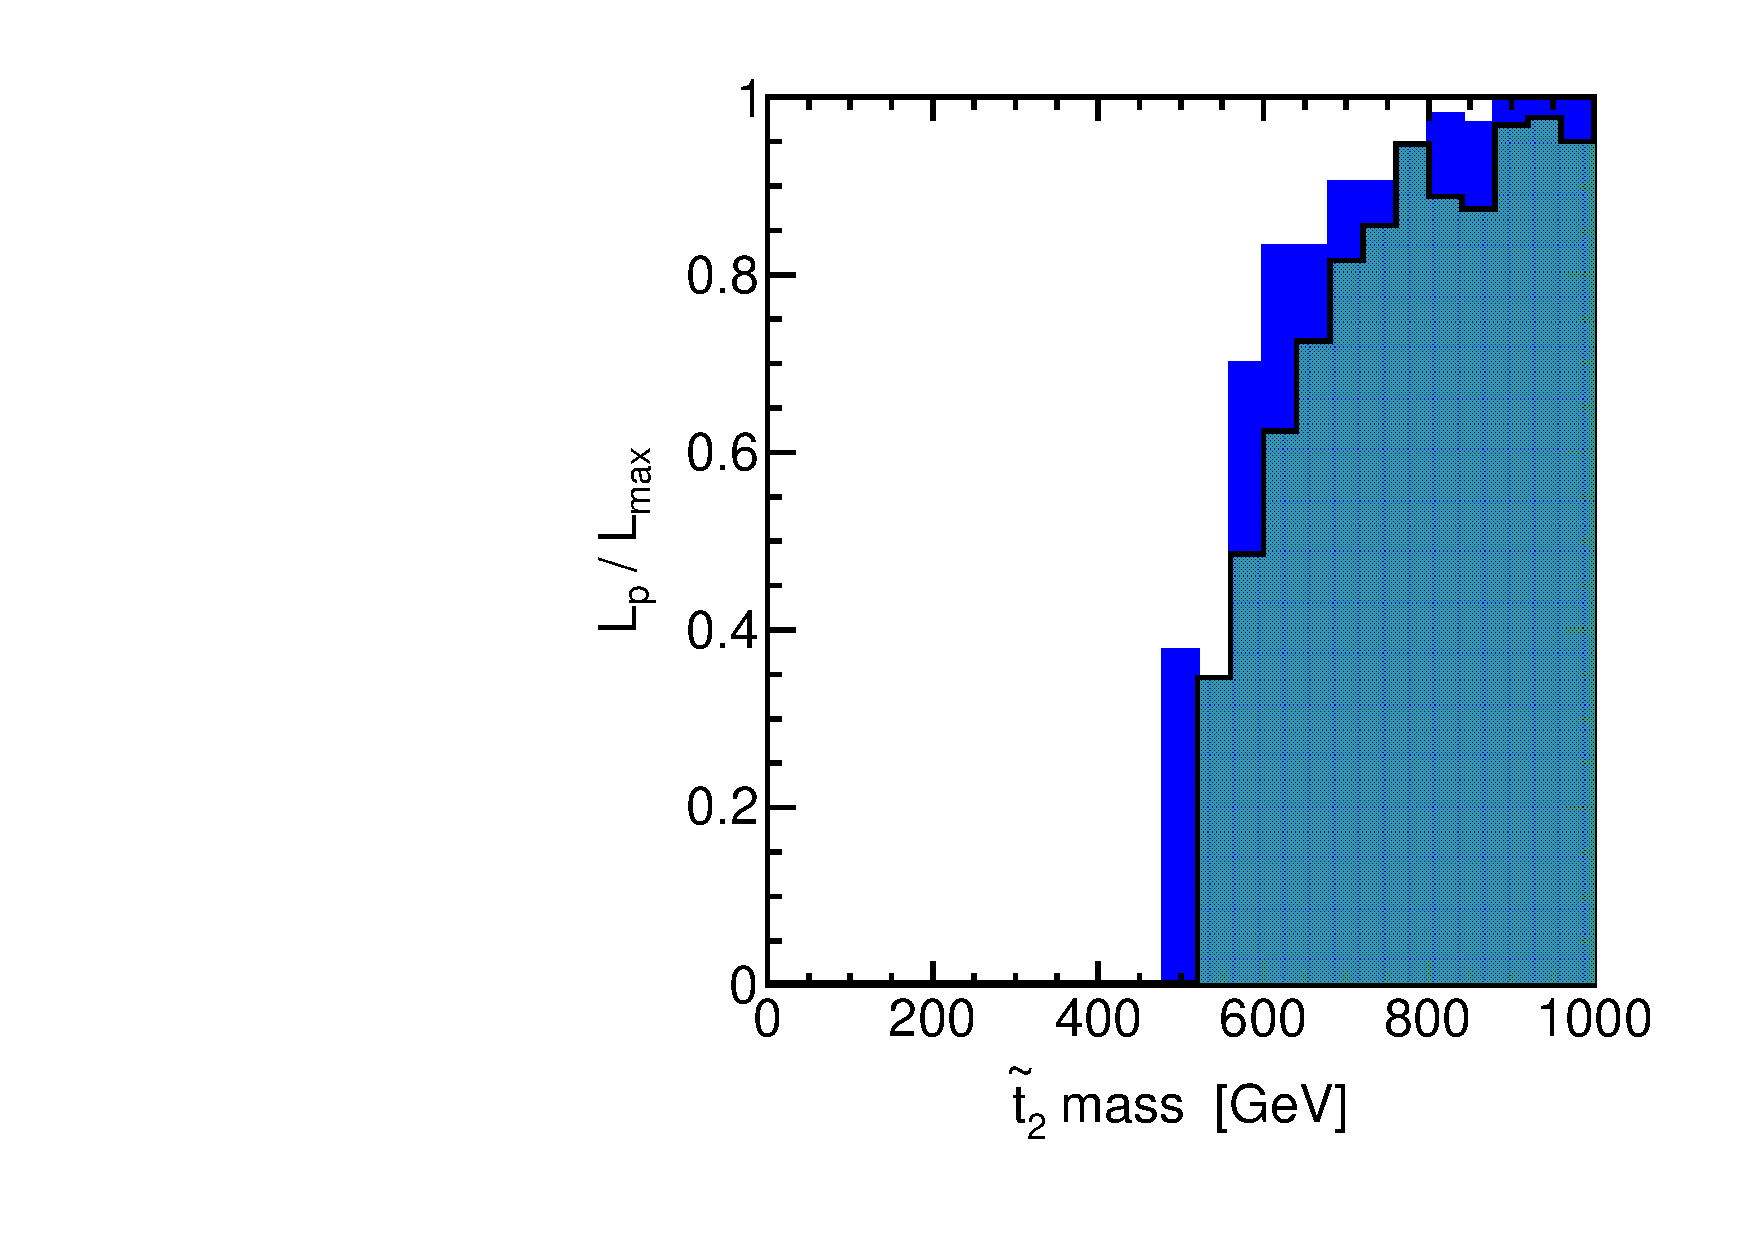
\includegraphics[height=5.5cm]{figs/fig_t_2.pdf} \\
\caption{Squark masses.}
\label{default}
\end{center}
\end{figure}


\begin{figure}[htbp]
\begin{center}
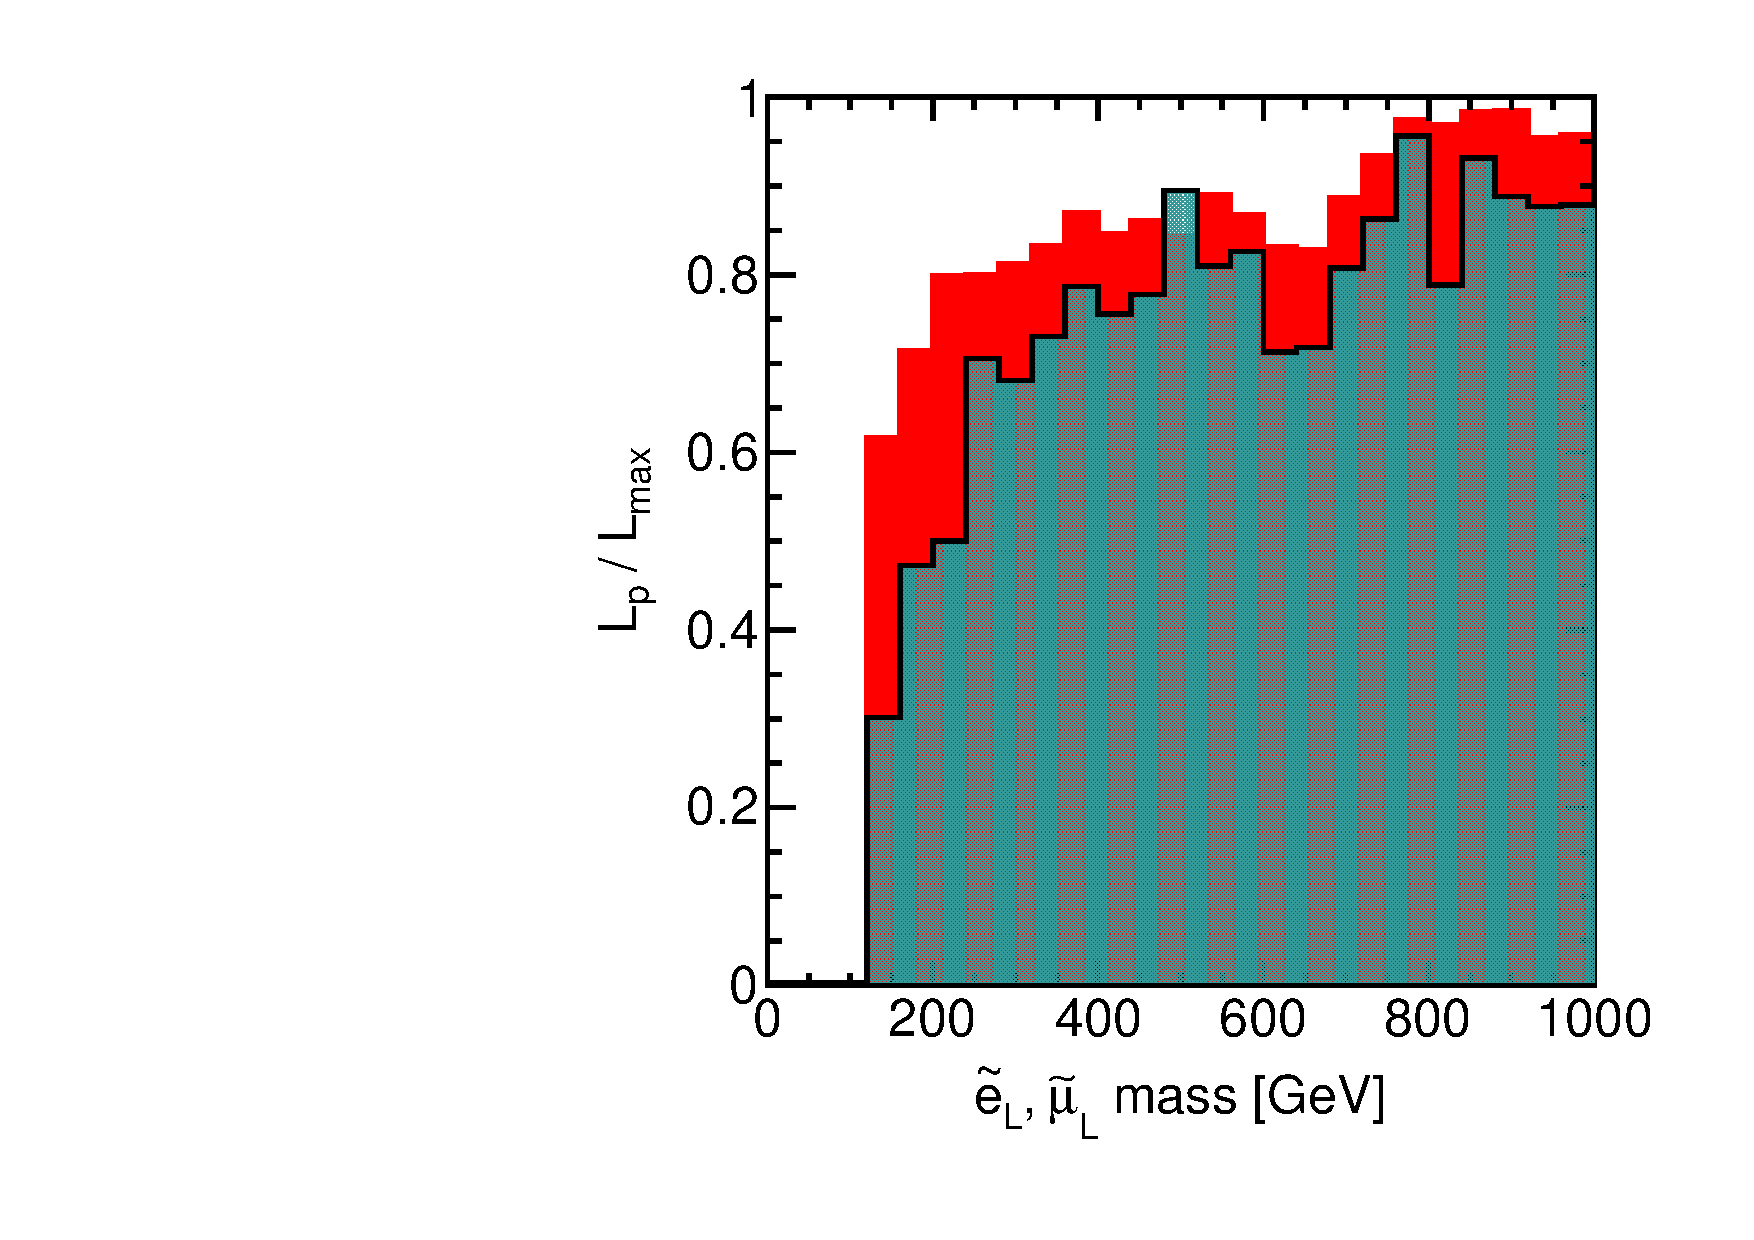
\includegraphics[height=5.5cm]{figs/fig_e_L.pdf} 
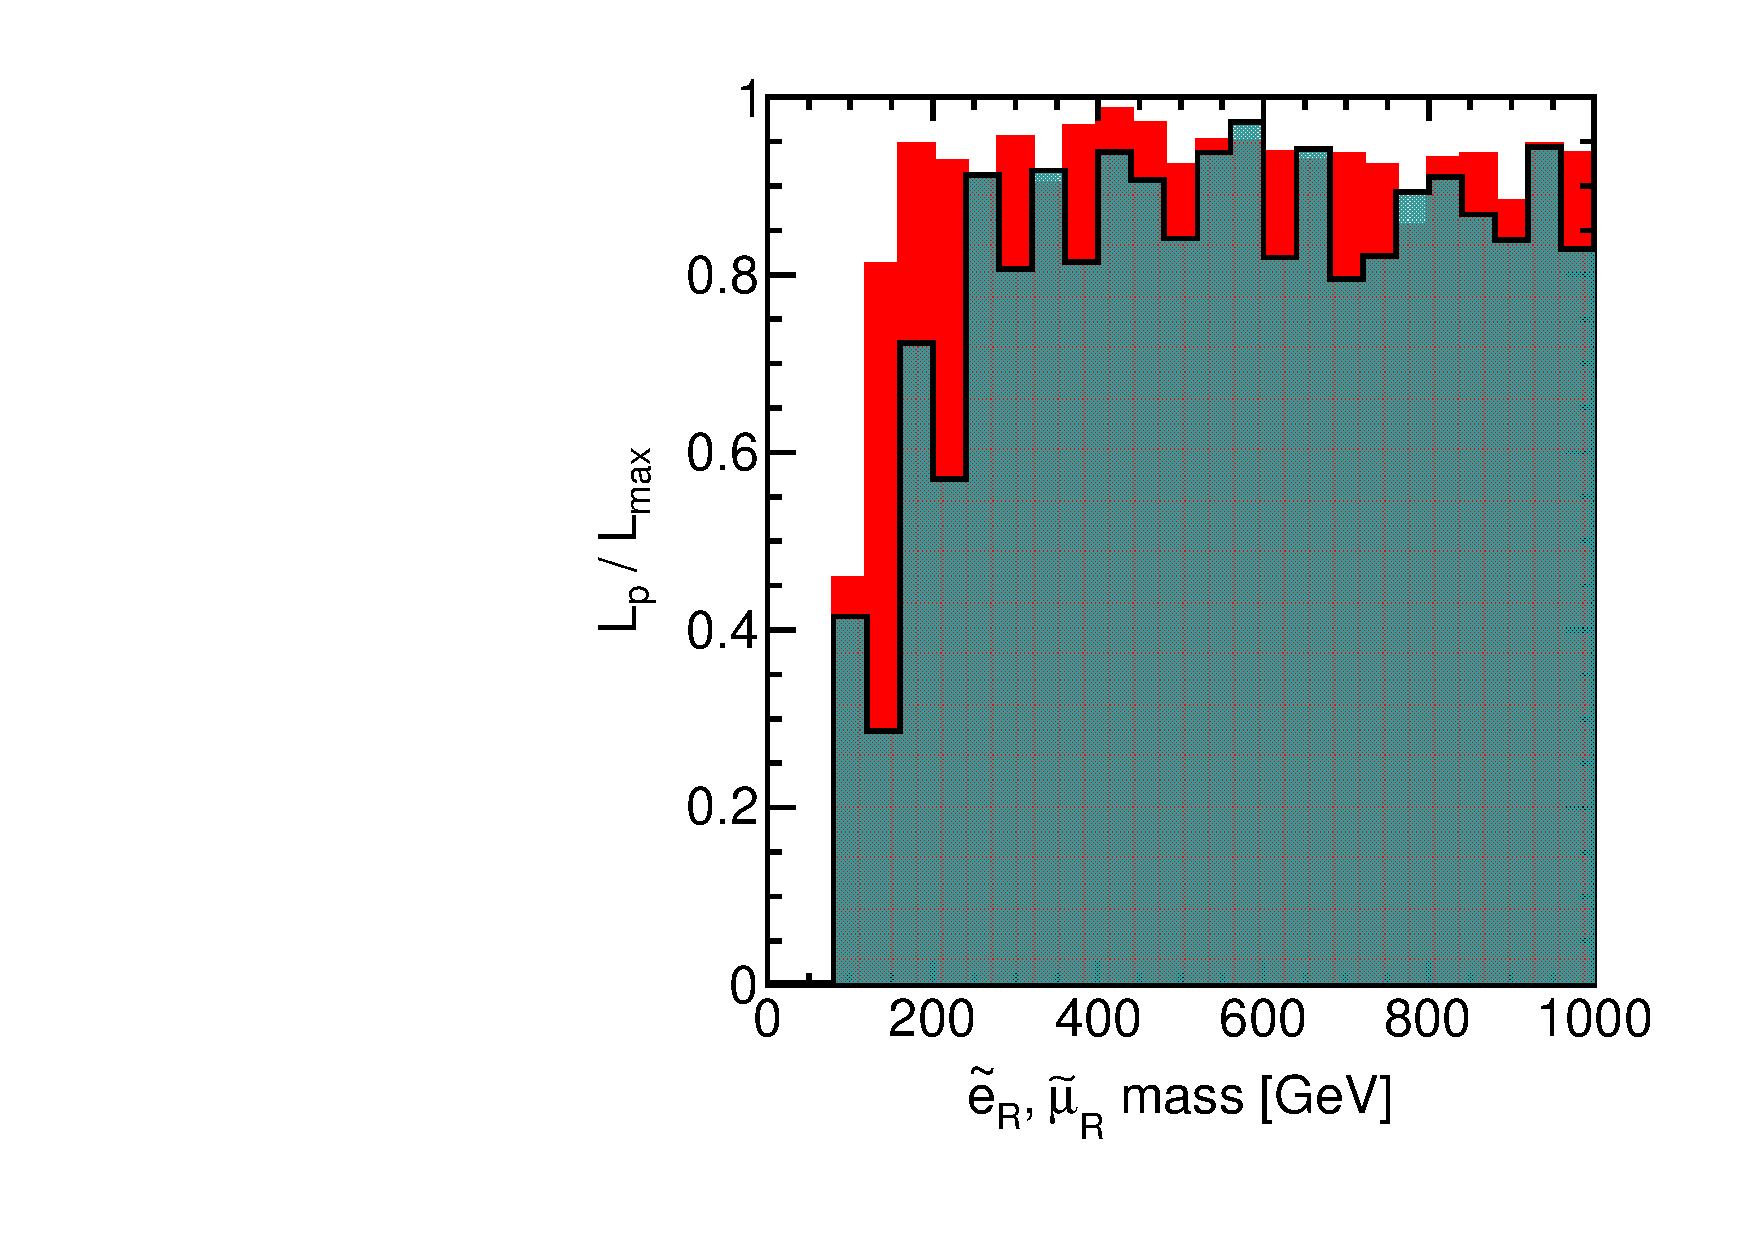
\includegraphics[height=5.5cm]{figs/fig_e_R.pdf} \\
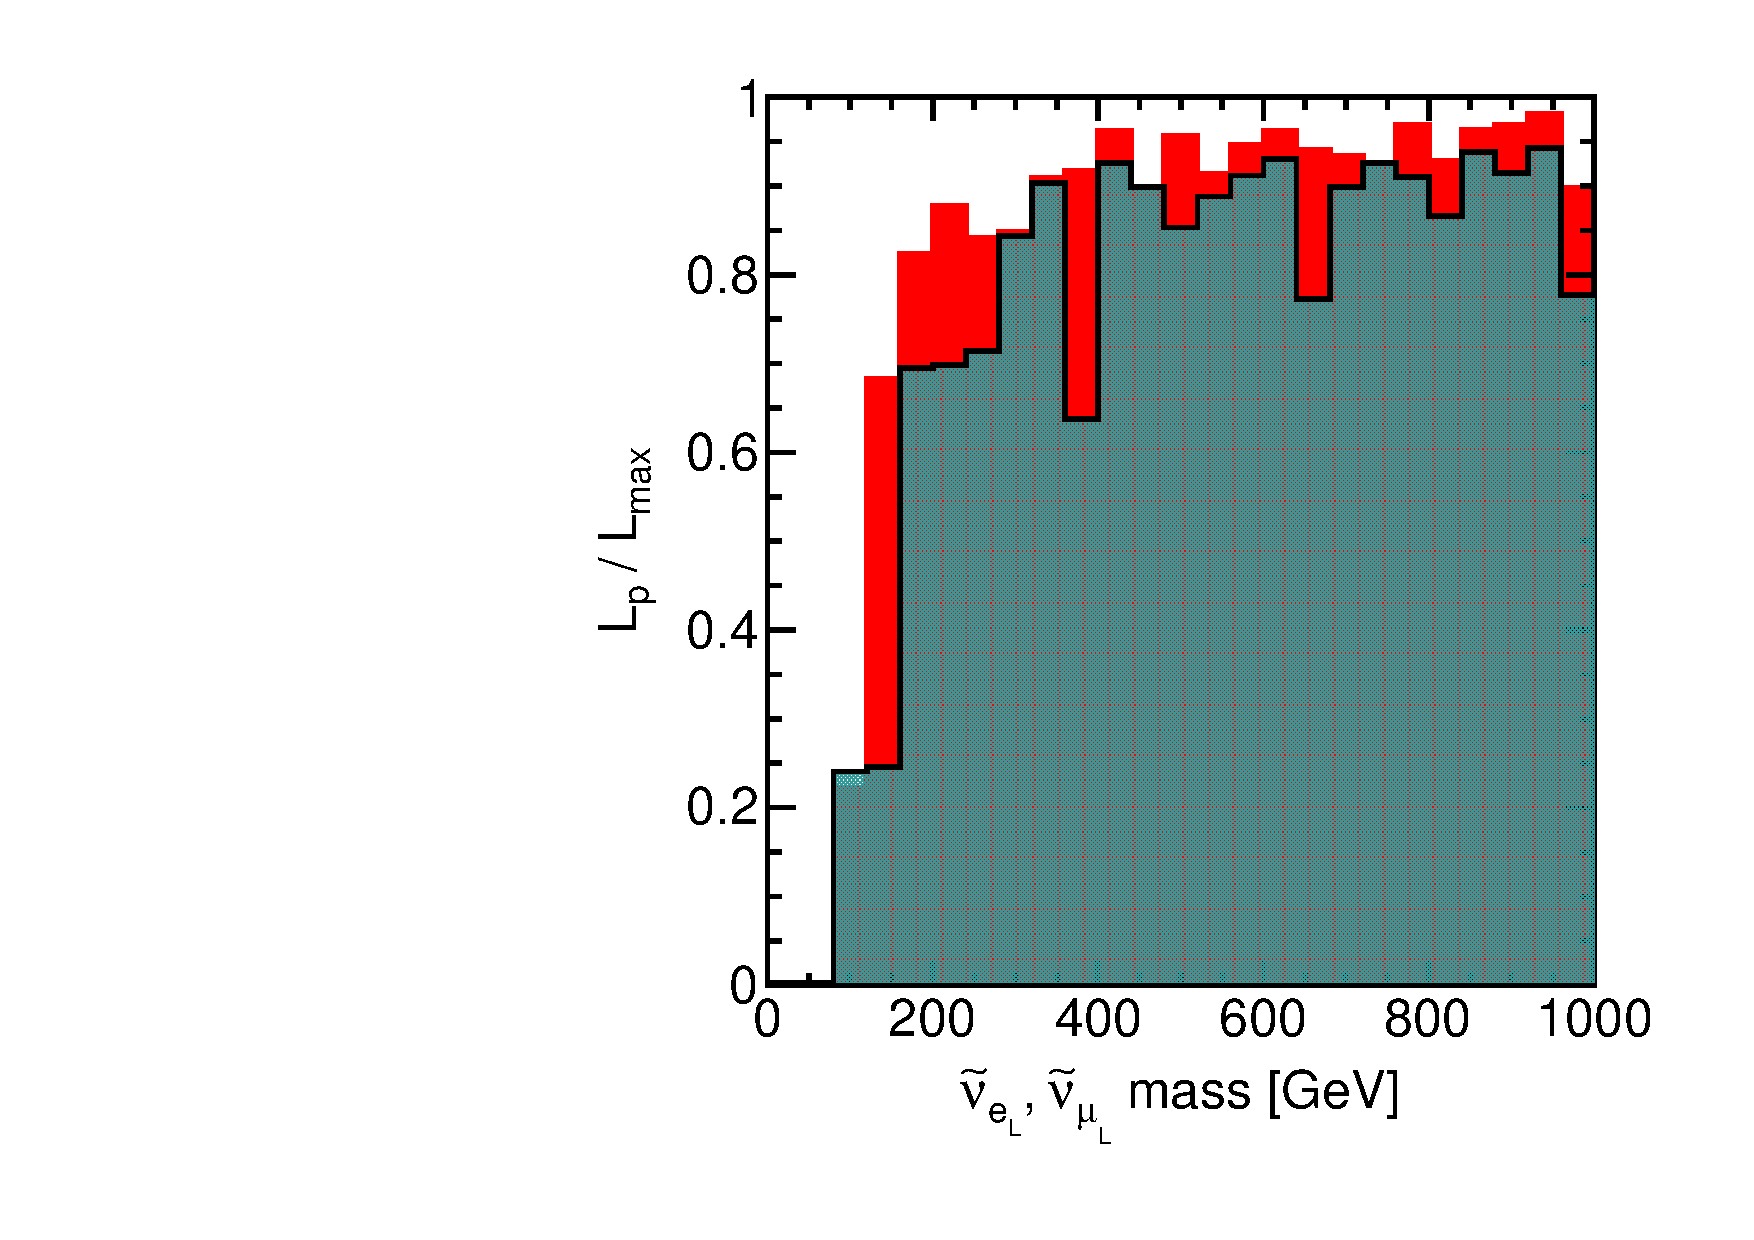
\includegraphics[height=5.5cm]{figs/fig_nu_e_L.pdf} 
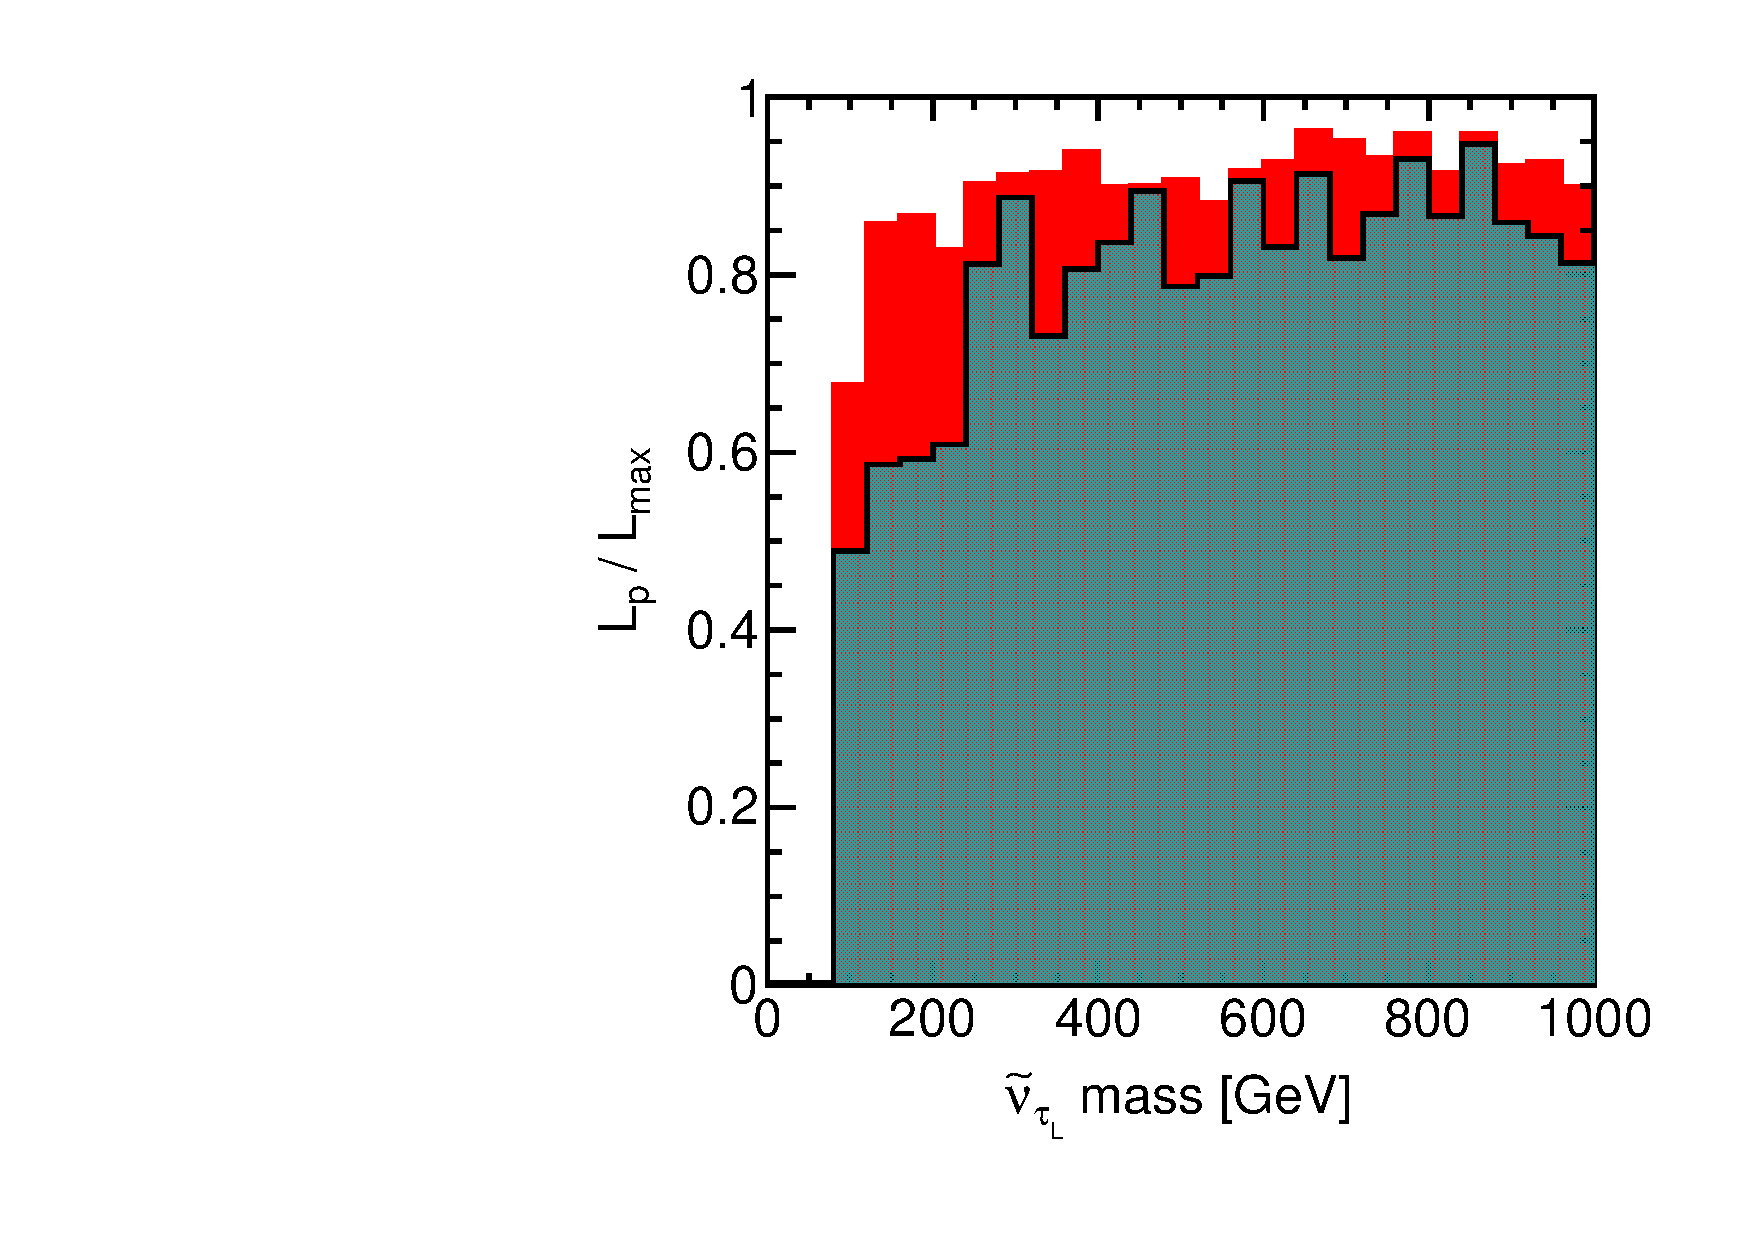
\includegraphics[height=5.5cm]{figs/fig_nu_tau_L.pdf} \\
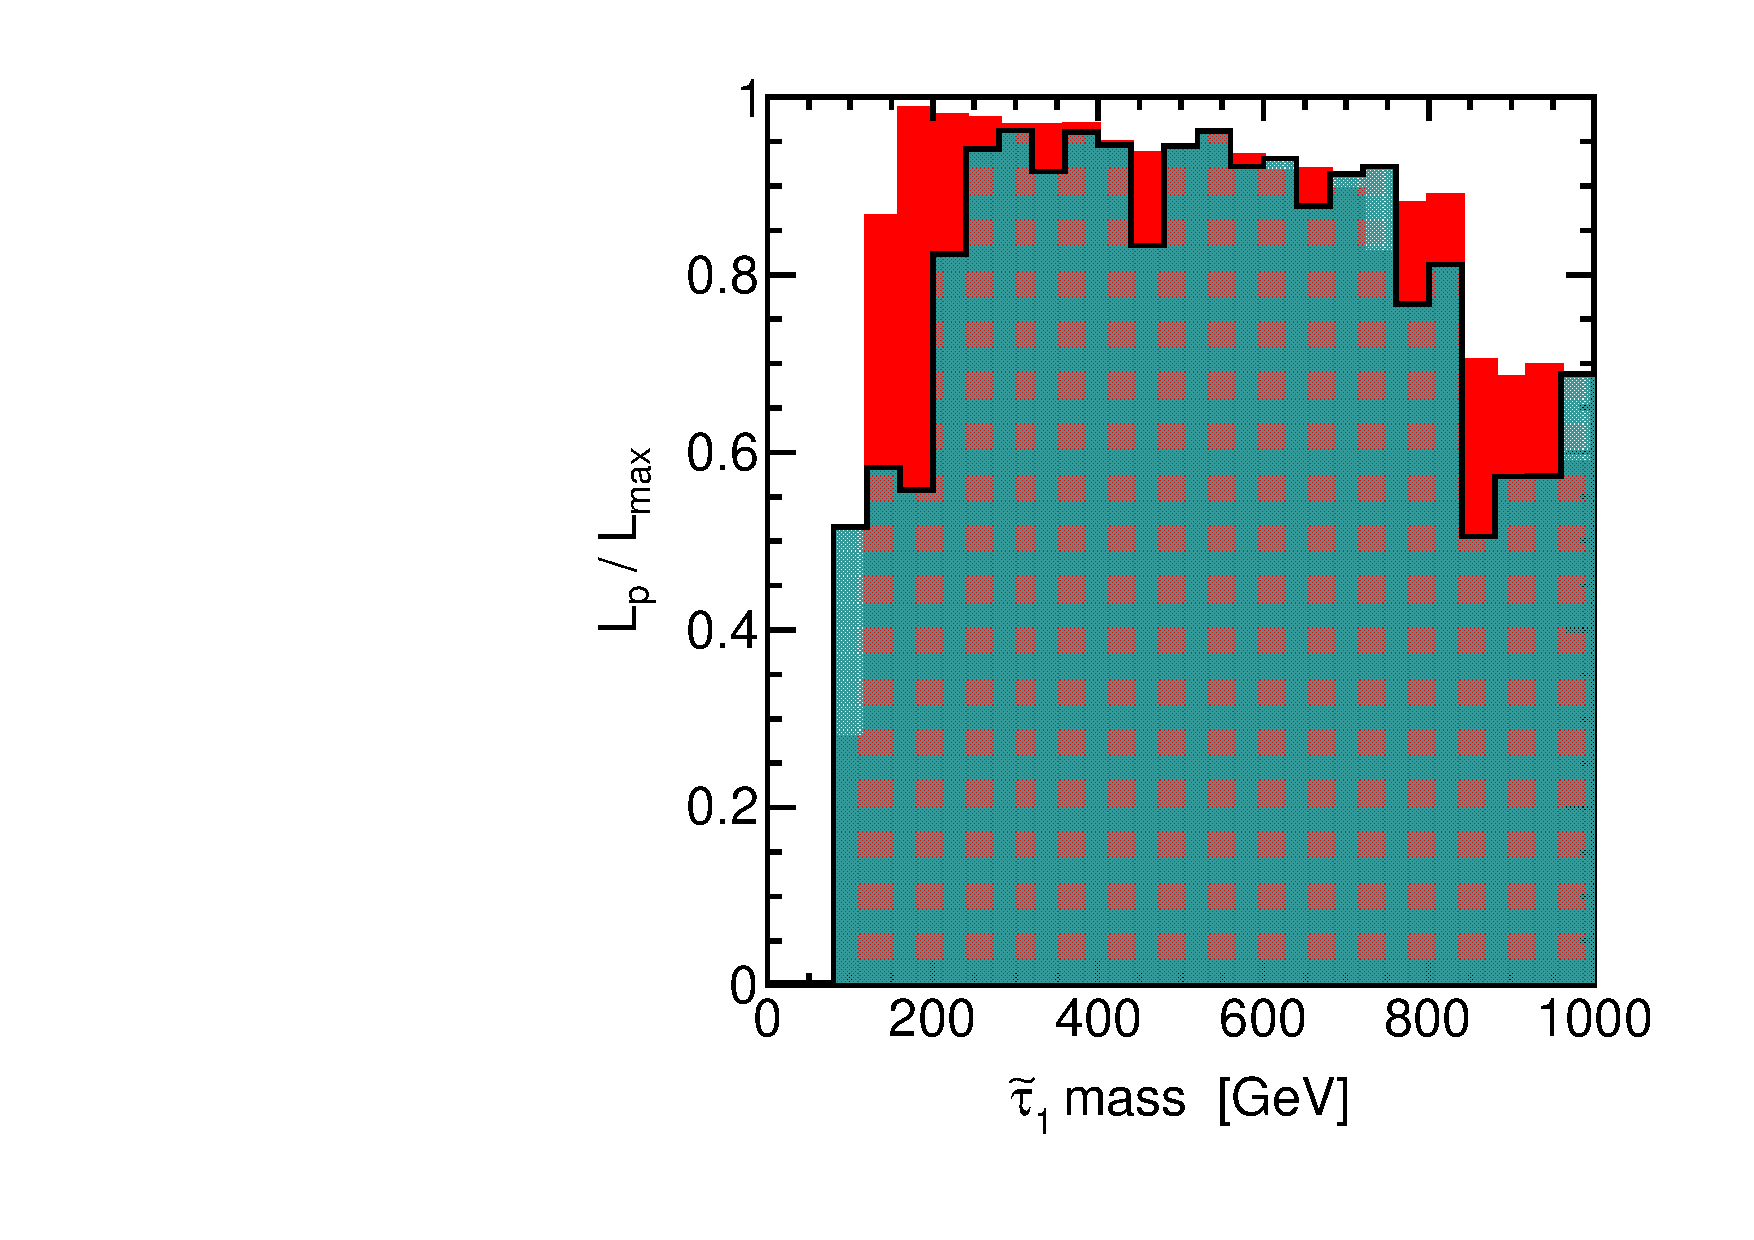
\includegraphics[height=5.5cm]{figs/fig_tau_1.pdf} 
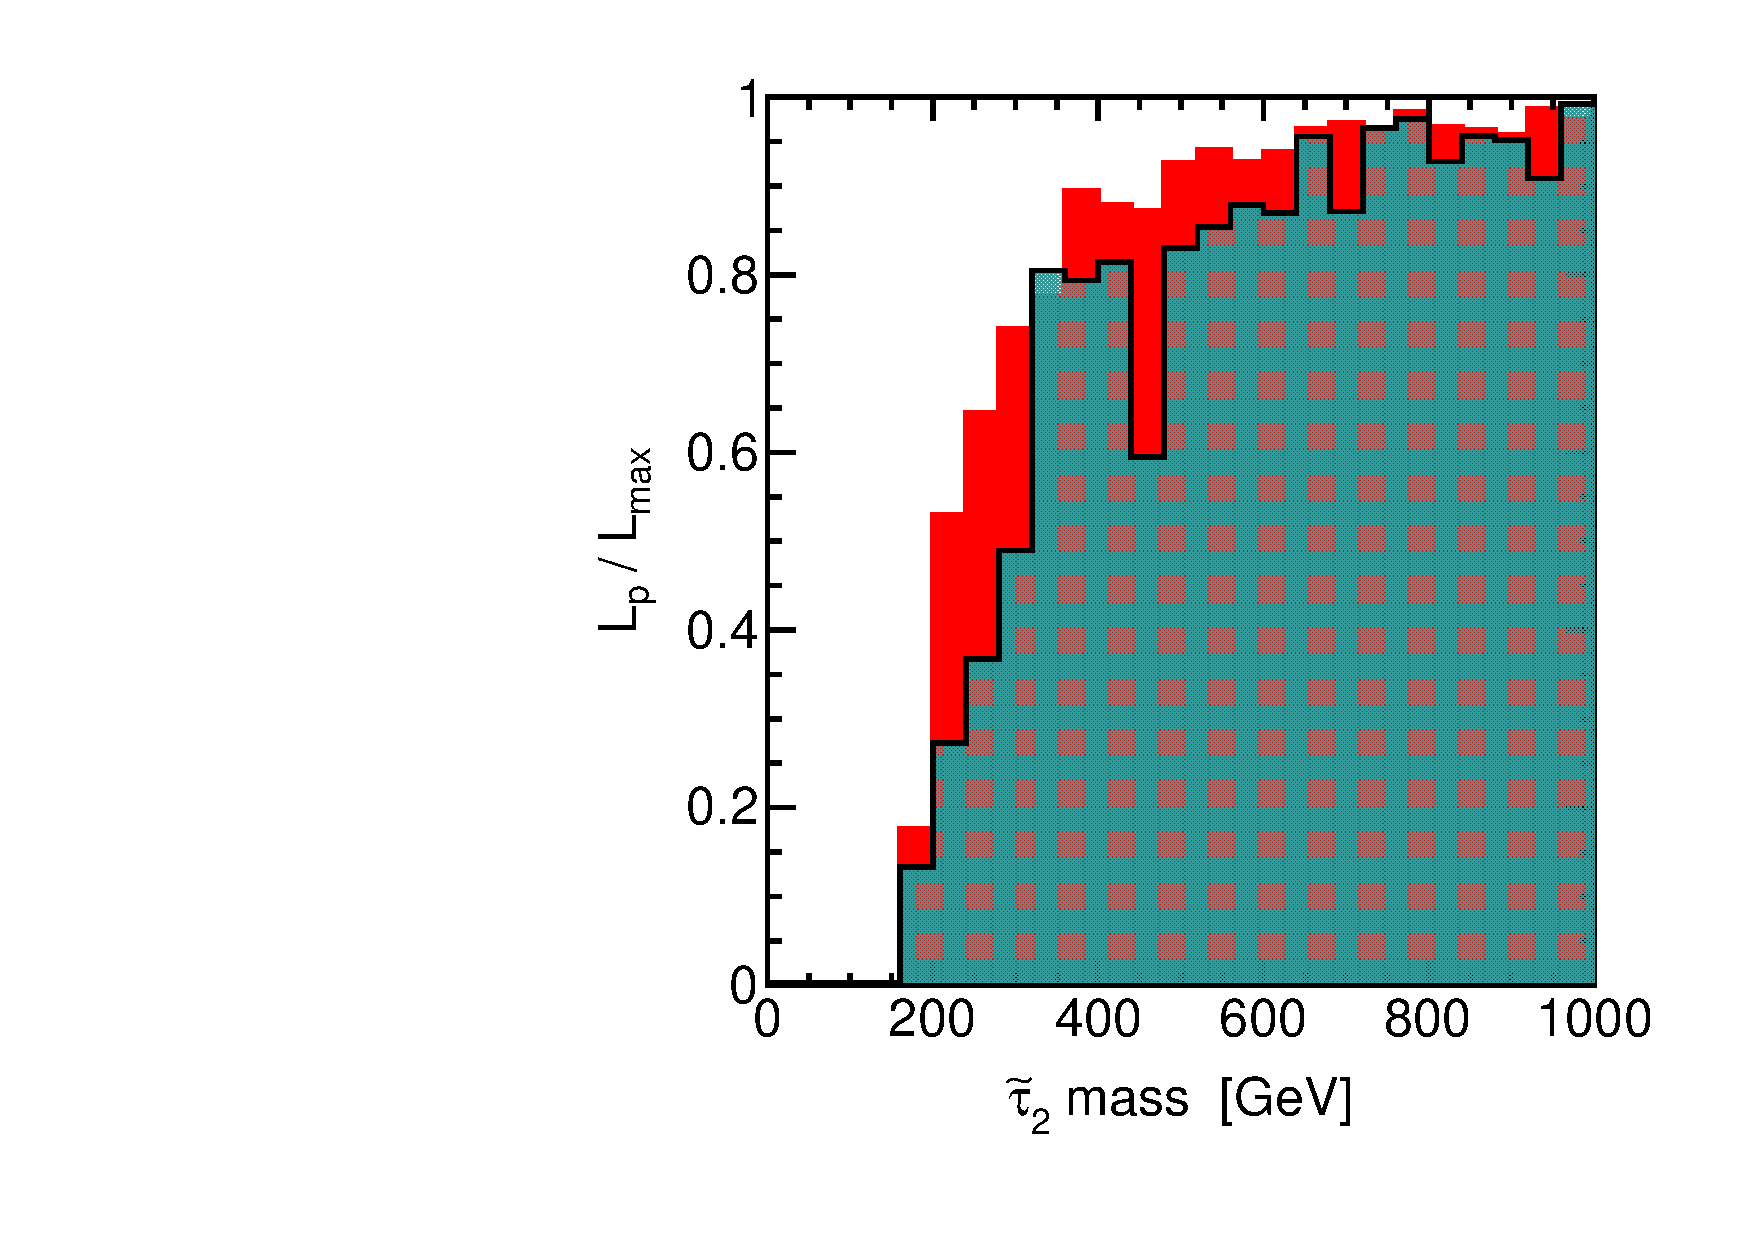
\includegraphics[height=5.5cm]{figs/fig_tau_2.pdf}
\caption{Slepton masses.}
\label{default}
\end{center}
\end{figure}


\begin{figure}[htbp]
\begin{center}
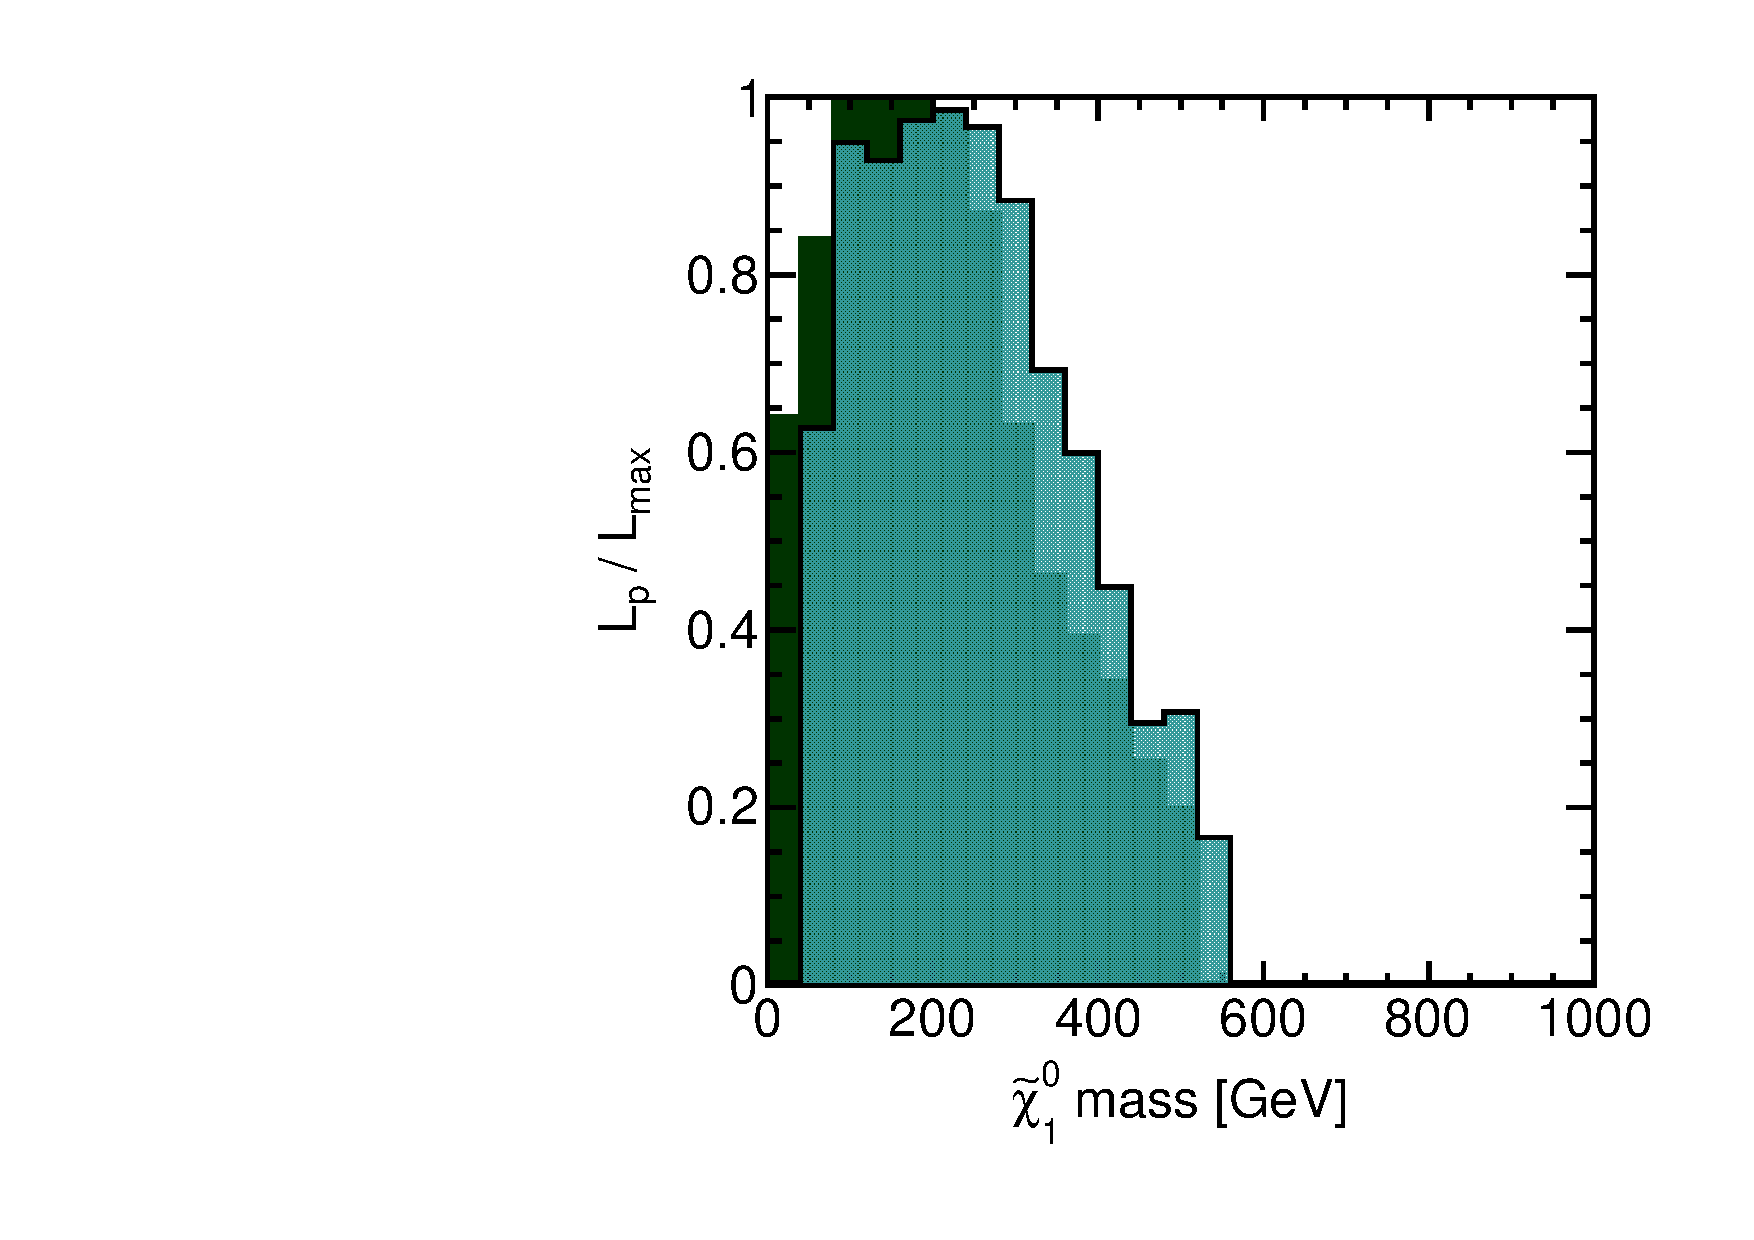
\includegraphics[height=5.5cm]{figs/fig_chi_1_0.pdf} 
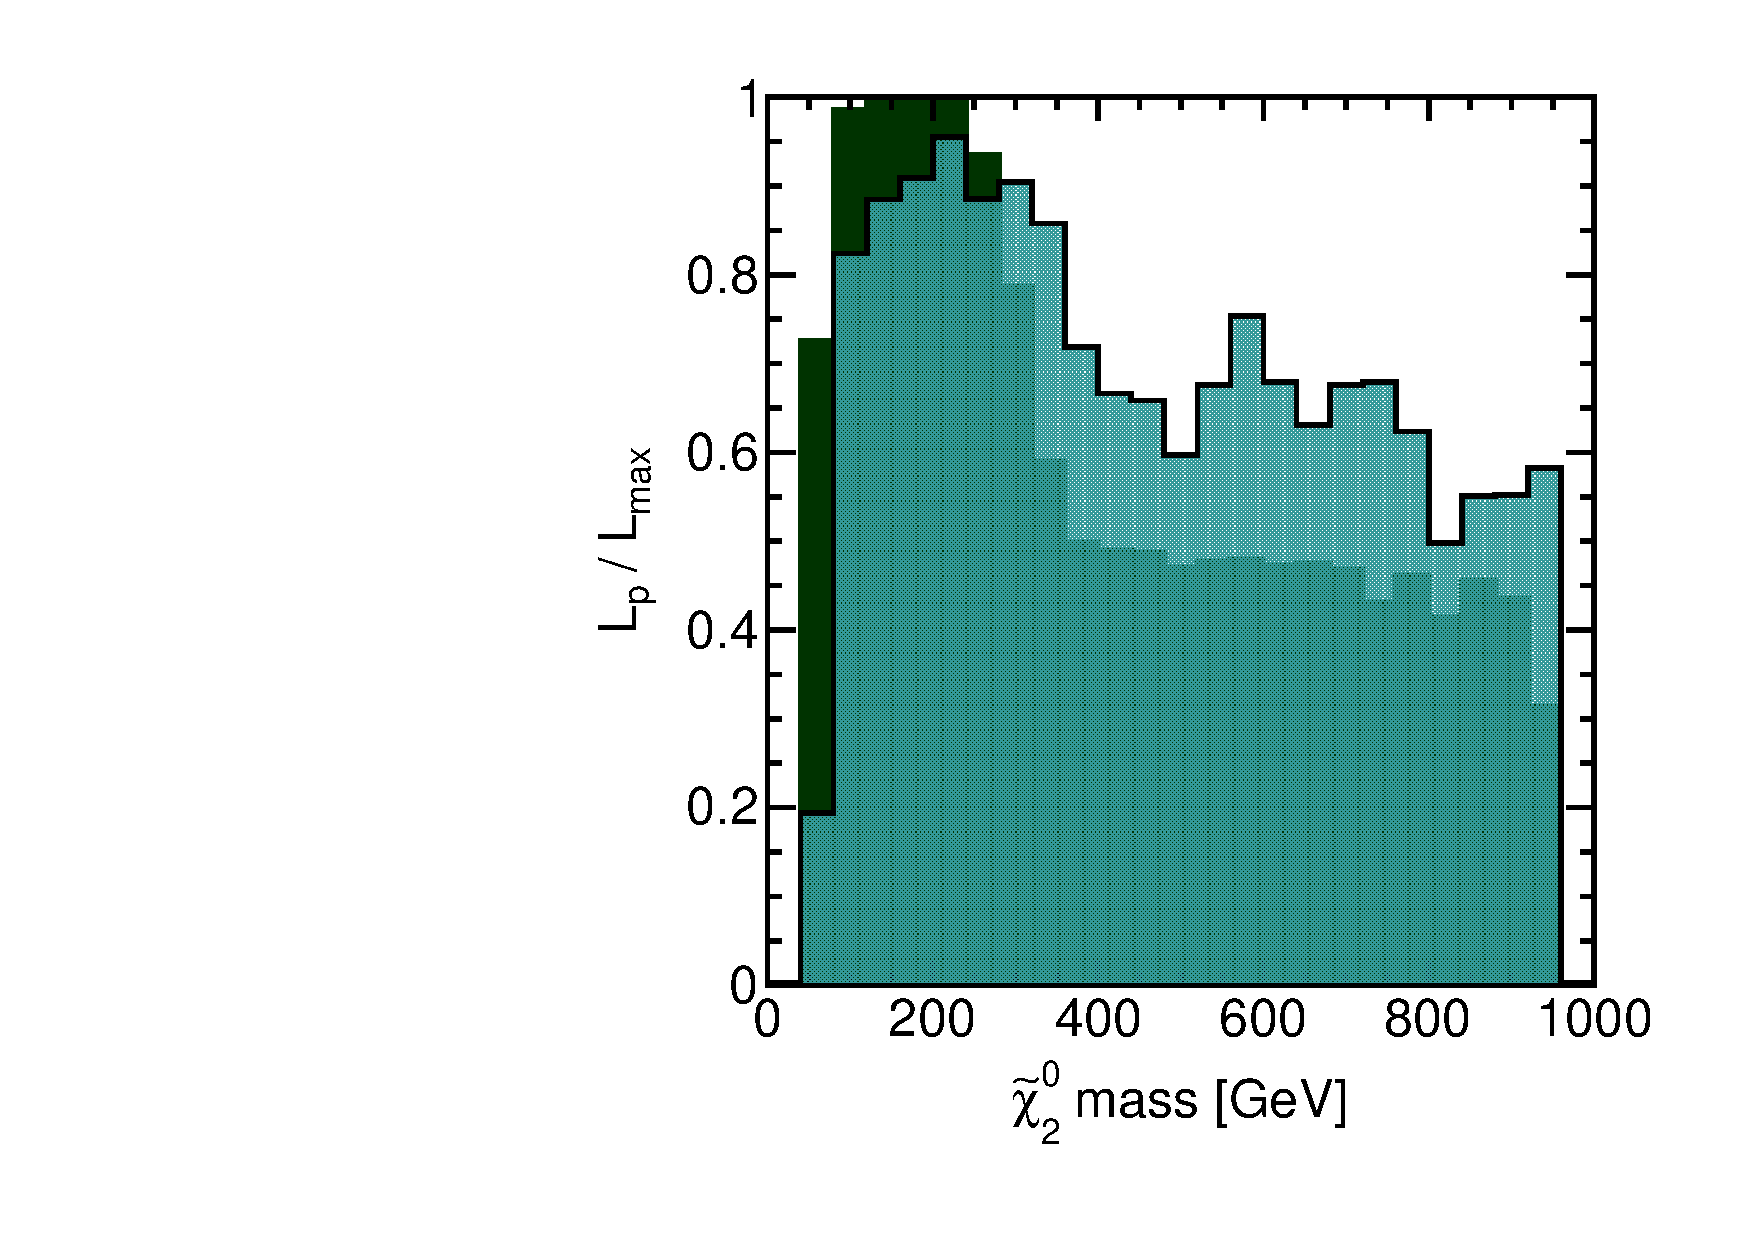
\includegraphics[height=5.5cm]{figs/fig_chi_2_0.pdf} \\
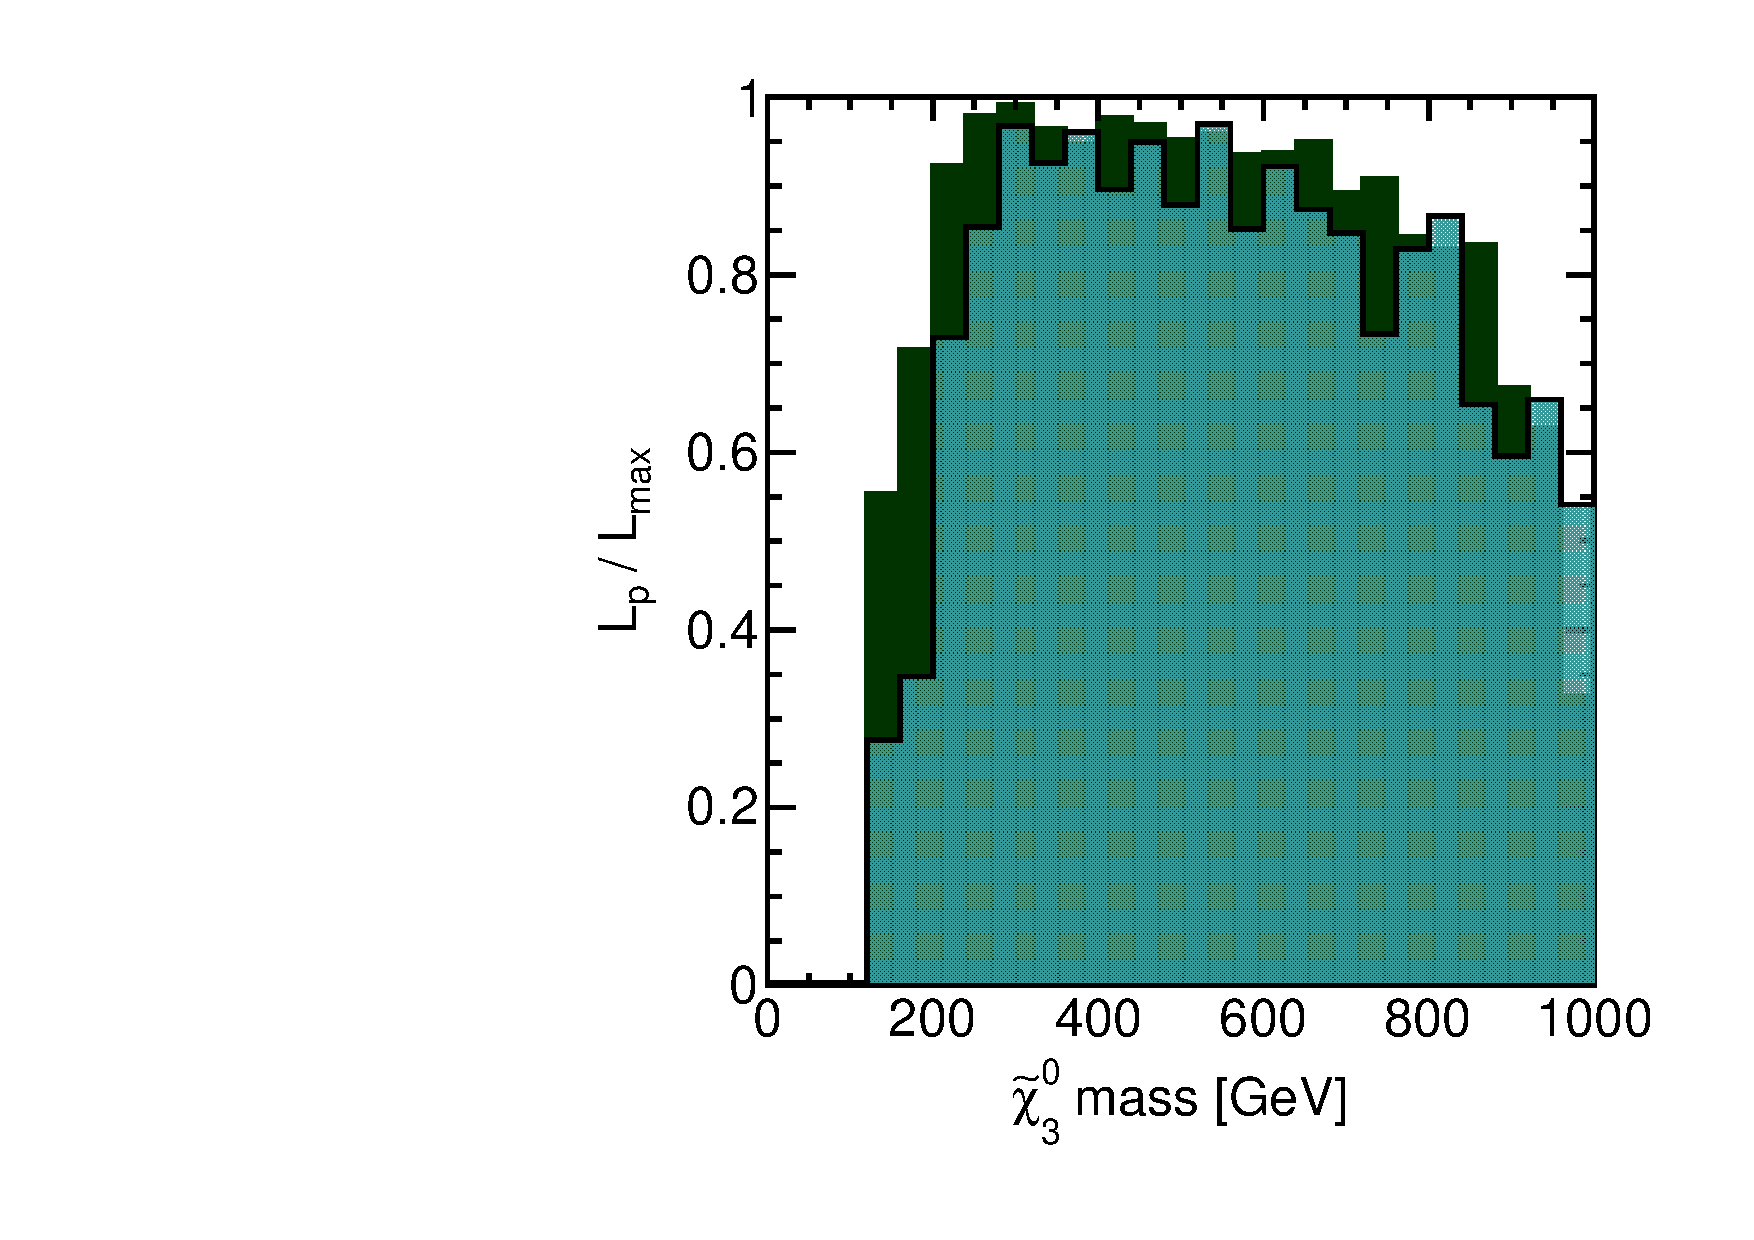
\includegraphics[height=5.5cm]{figs/fig_chi_3_0.pdf} 
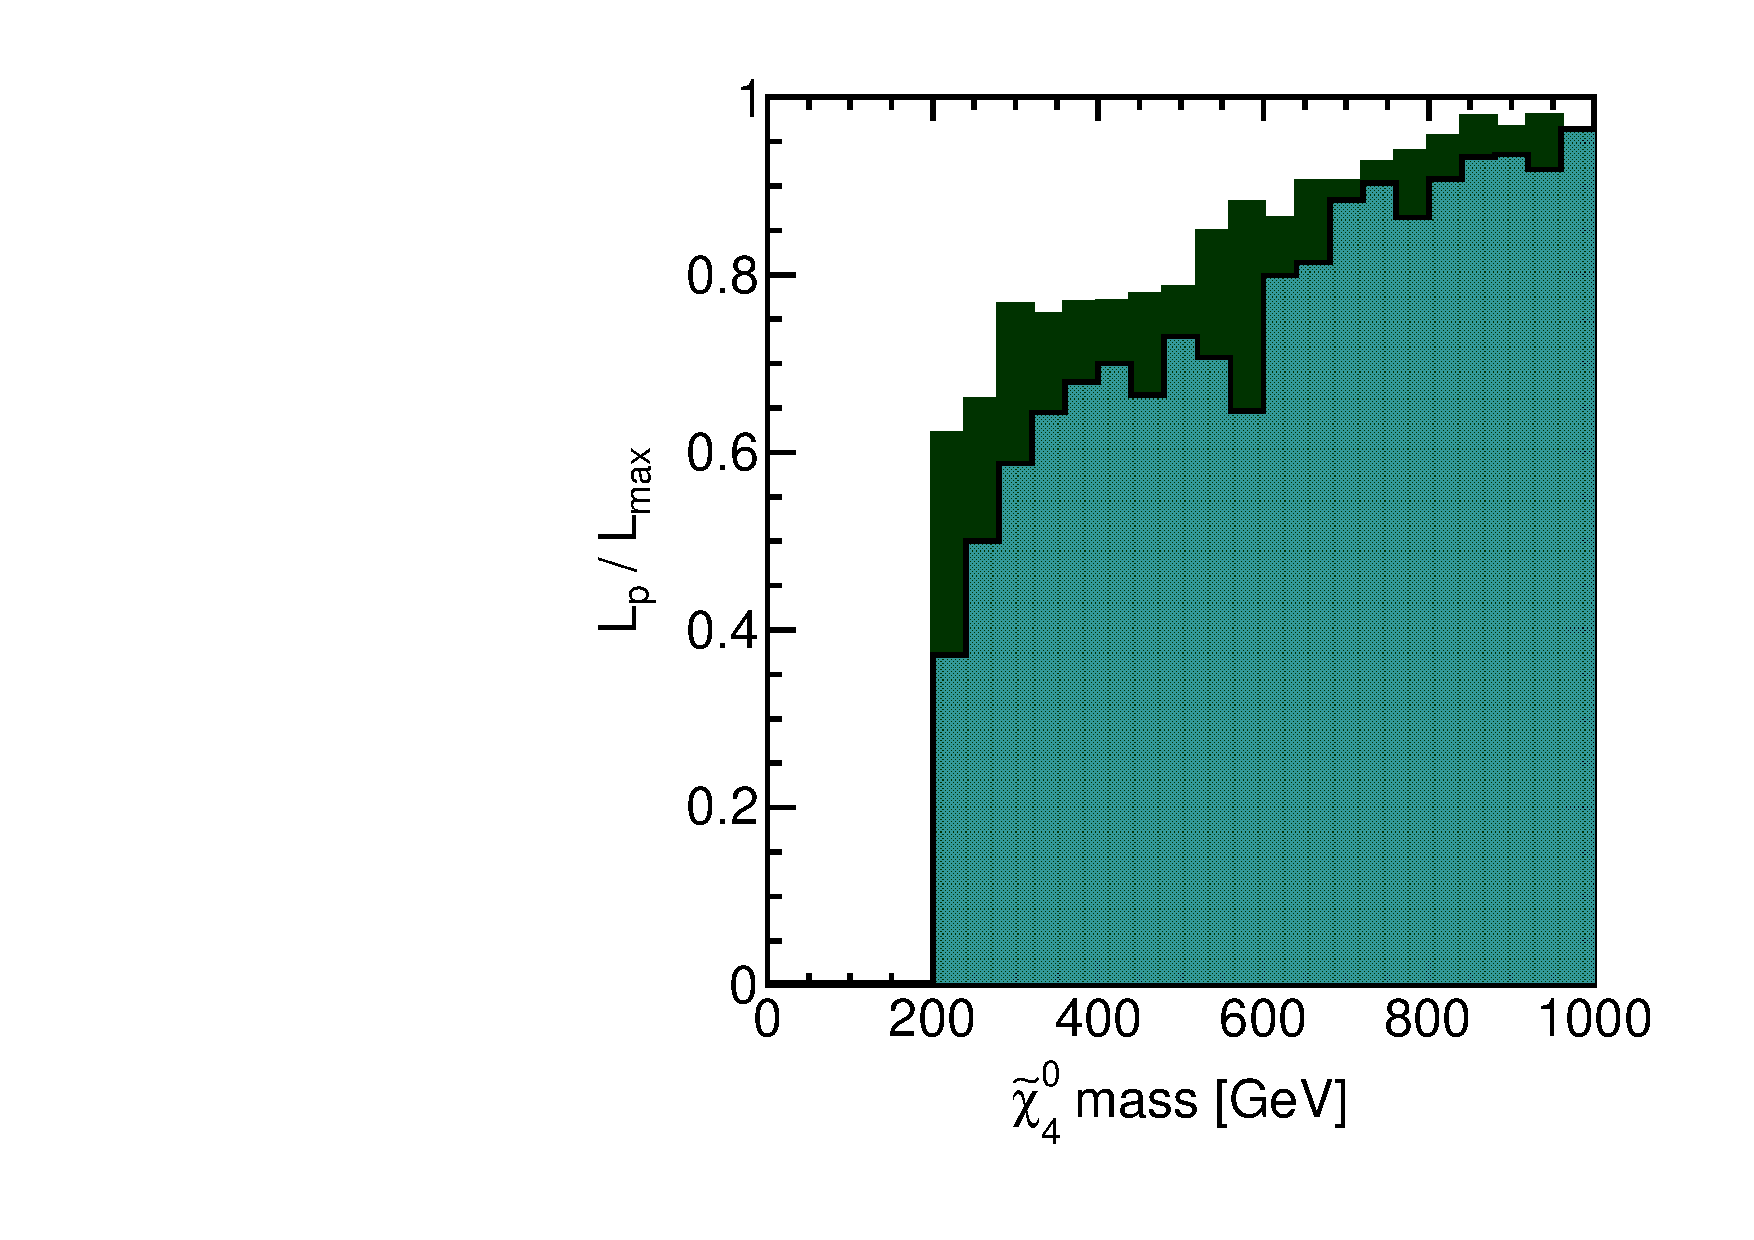
\includegraphics[height=5.5cm]{figs/fig_chi_4_0.pdf} 
\caption{Neutralino masses.}
\label{default}
\end{center}
\end{figure}

\begin{figure}[htbp]
\begin{center}
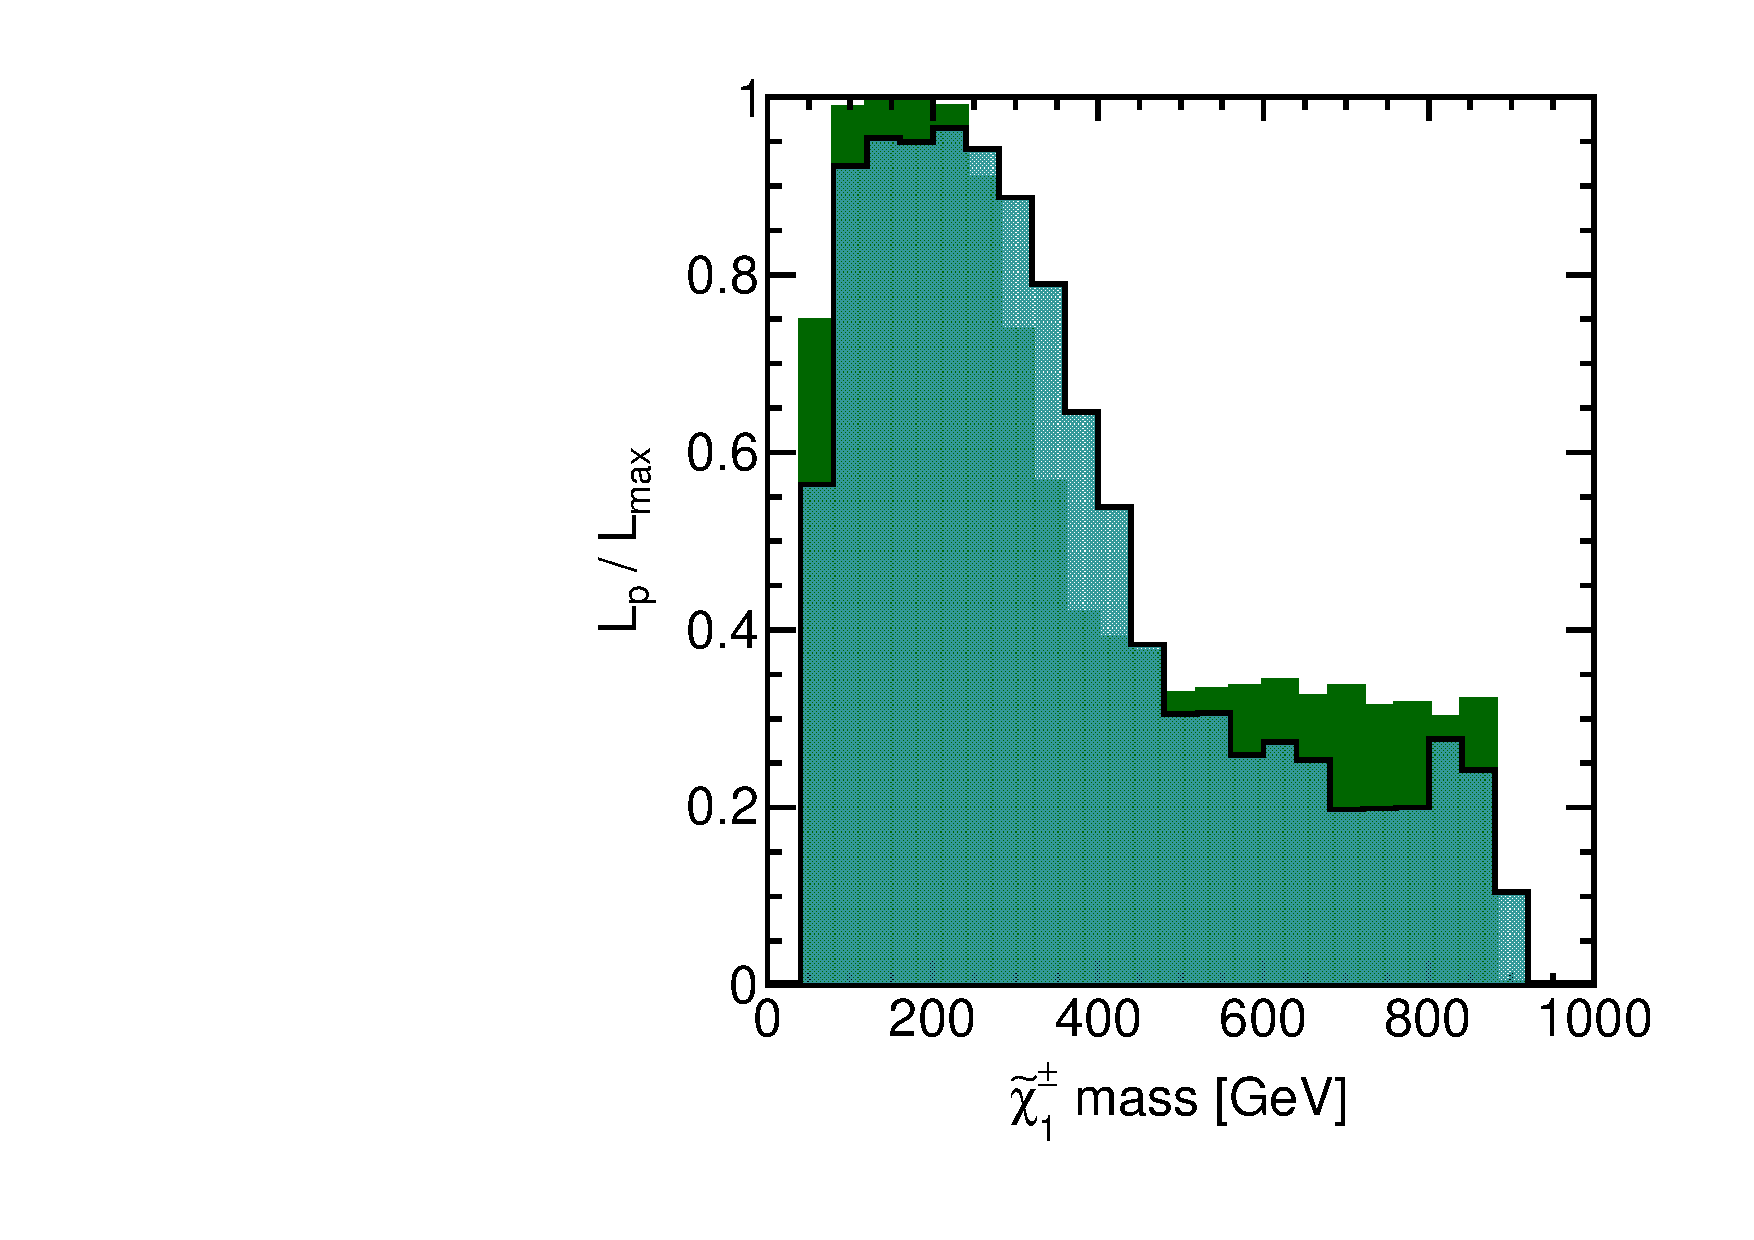
\includegraphics[height=5.5cm]{figs/fig_chi_1_pm.pdf} 
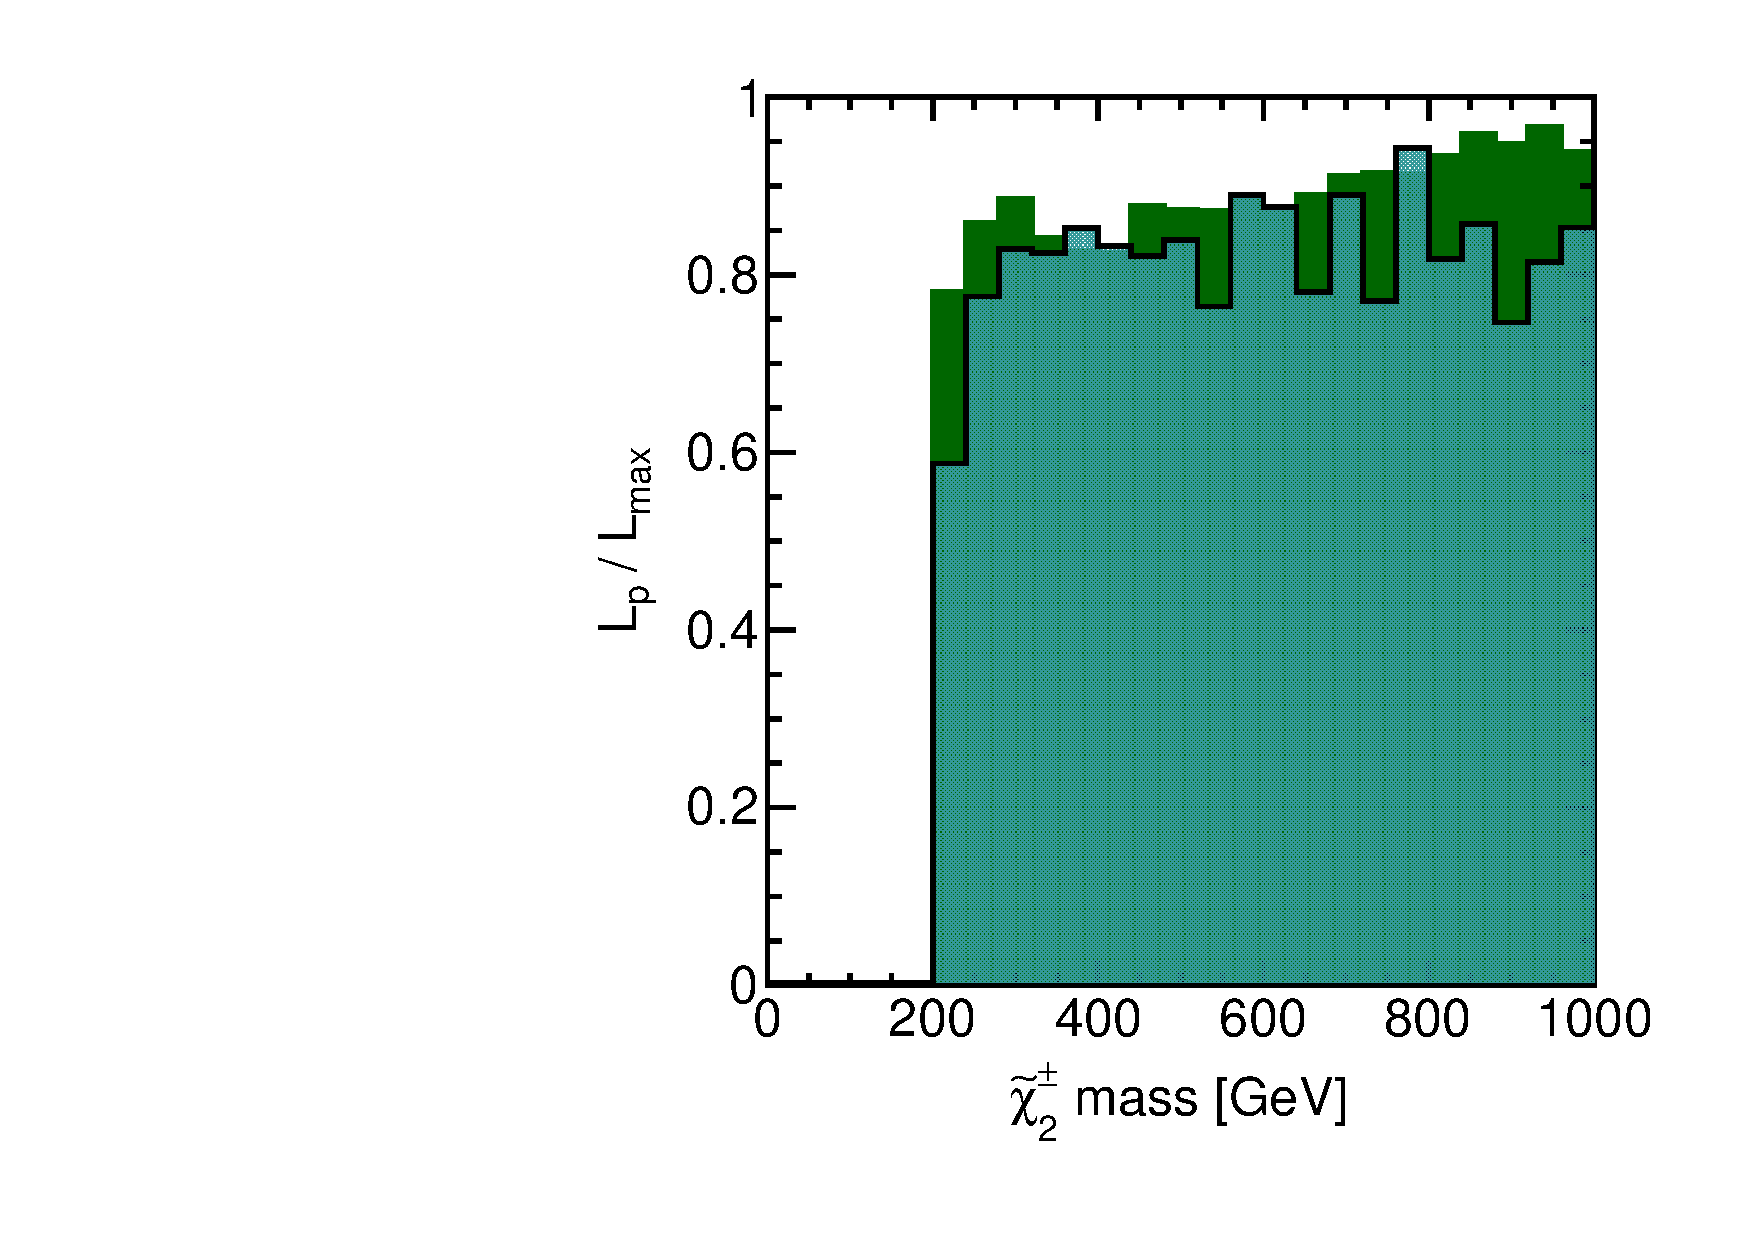
\includegraphics[height=5.5cm]{figs/fig_chi_2_pm.pdf}
\caption{Chargino masses}
\label{default}
\end{center}
\end{figure}


\begin{figure}[htbp]
\begin{center}
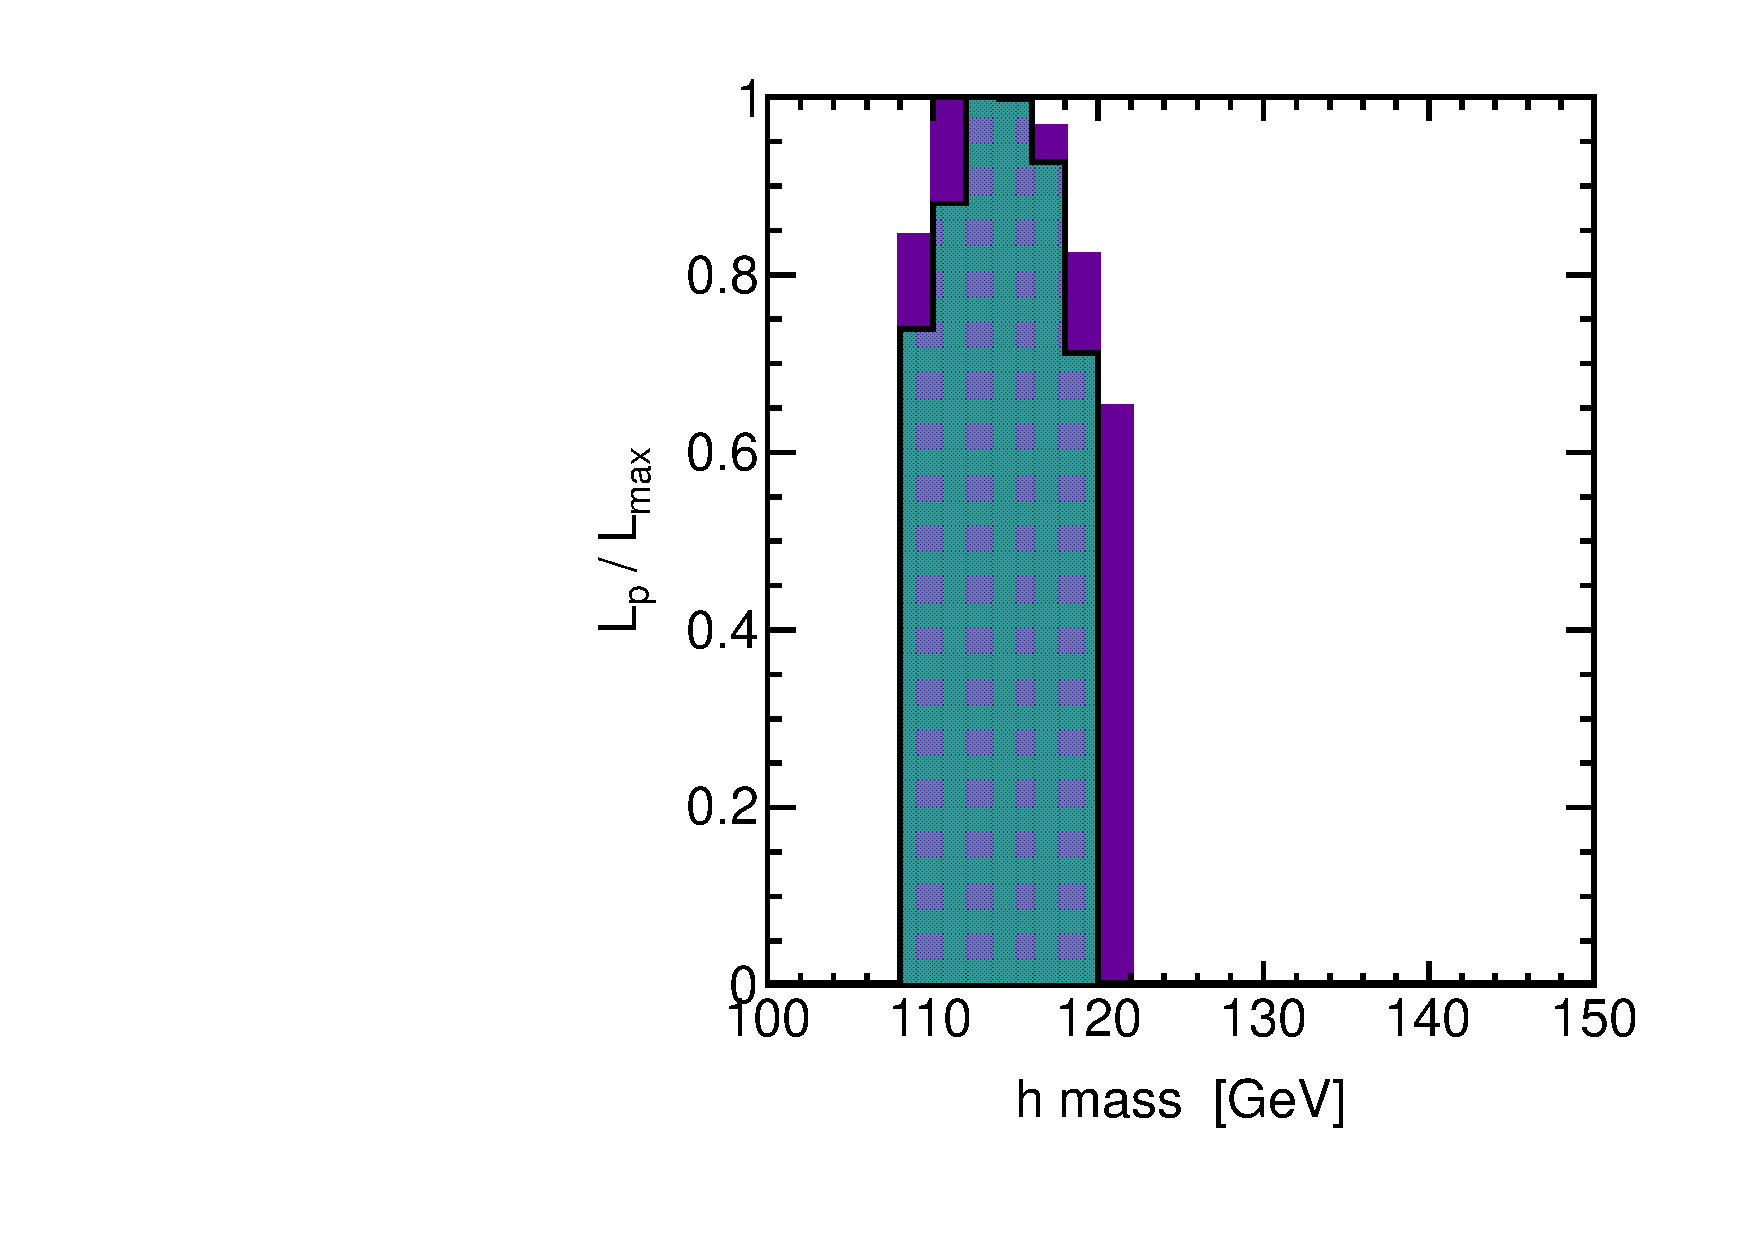
\includegraphics[height=5.5cm]{figs/fig_h.pdf} 
\includegraphics[height=5.5cm]{figs/fig_H.pdf} \\
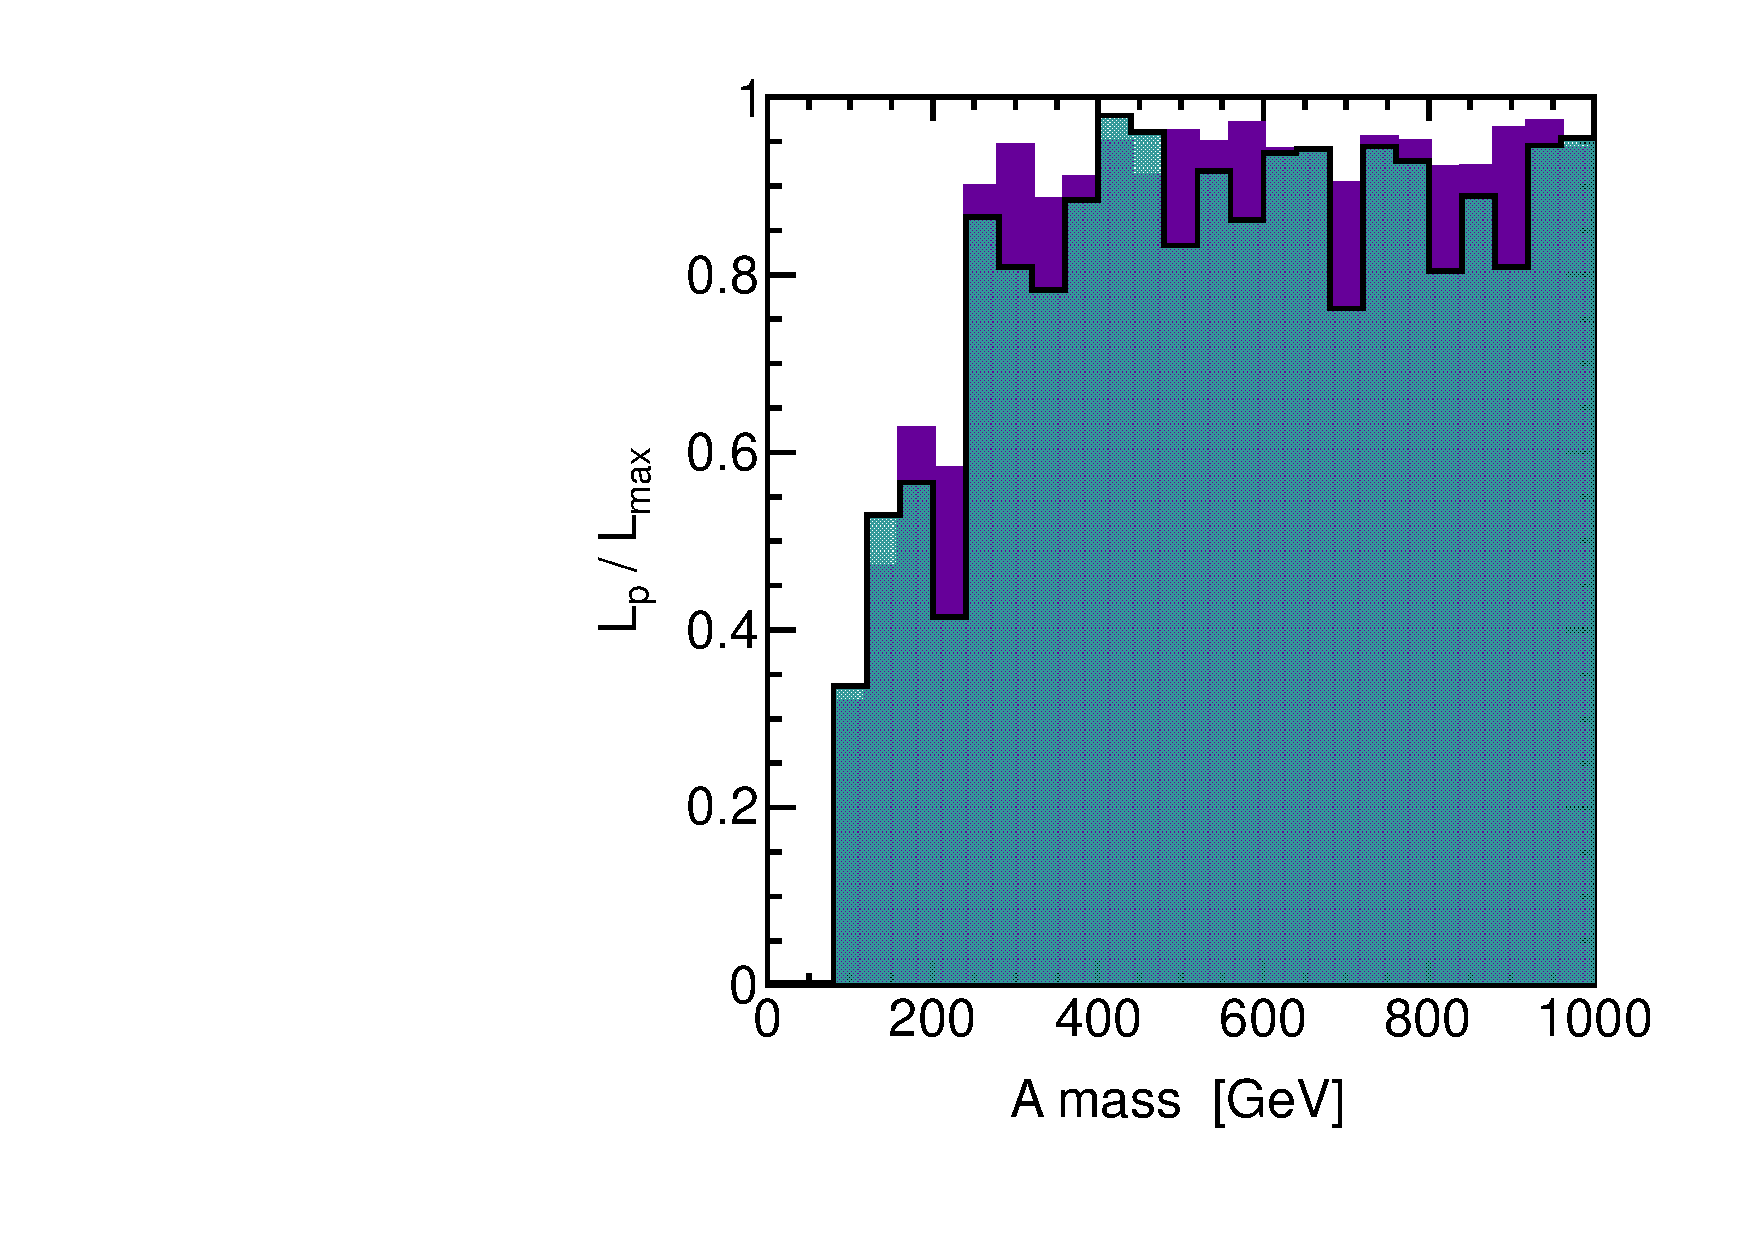
\includegraphics[height=5.5cm]{figs/fig_A.pdf} 
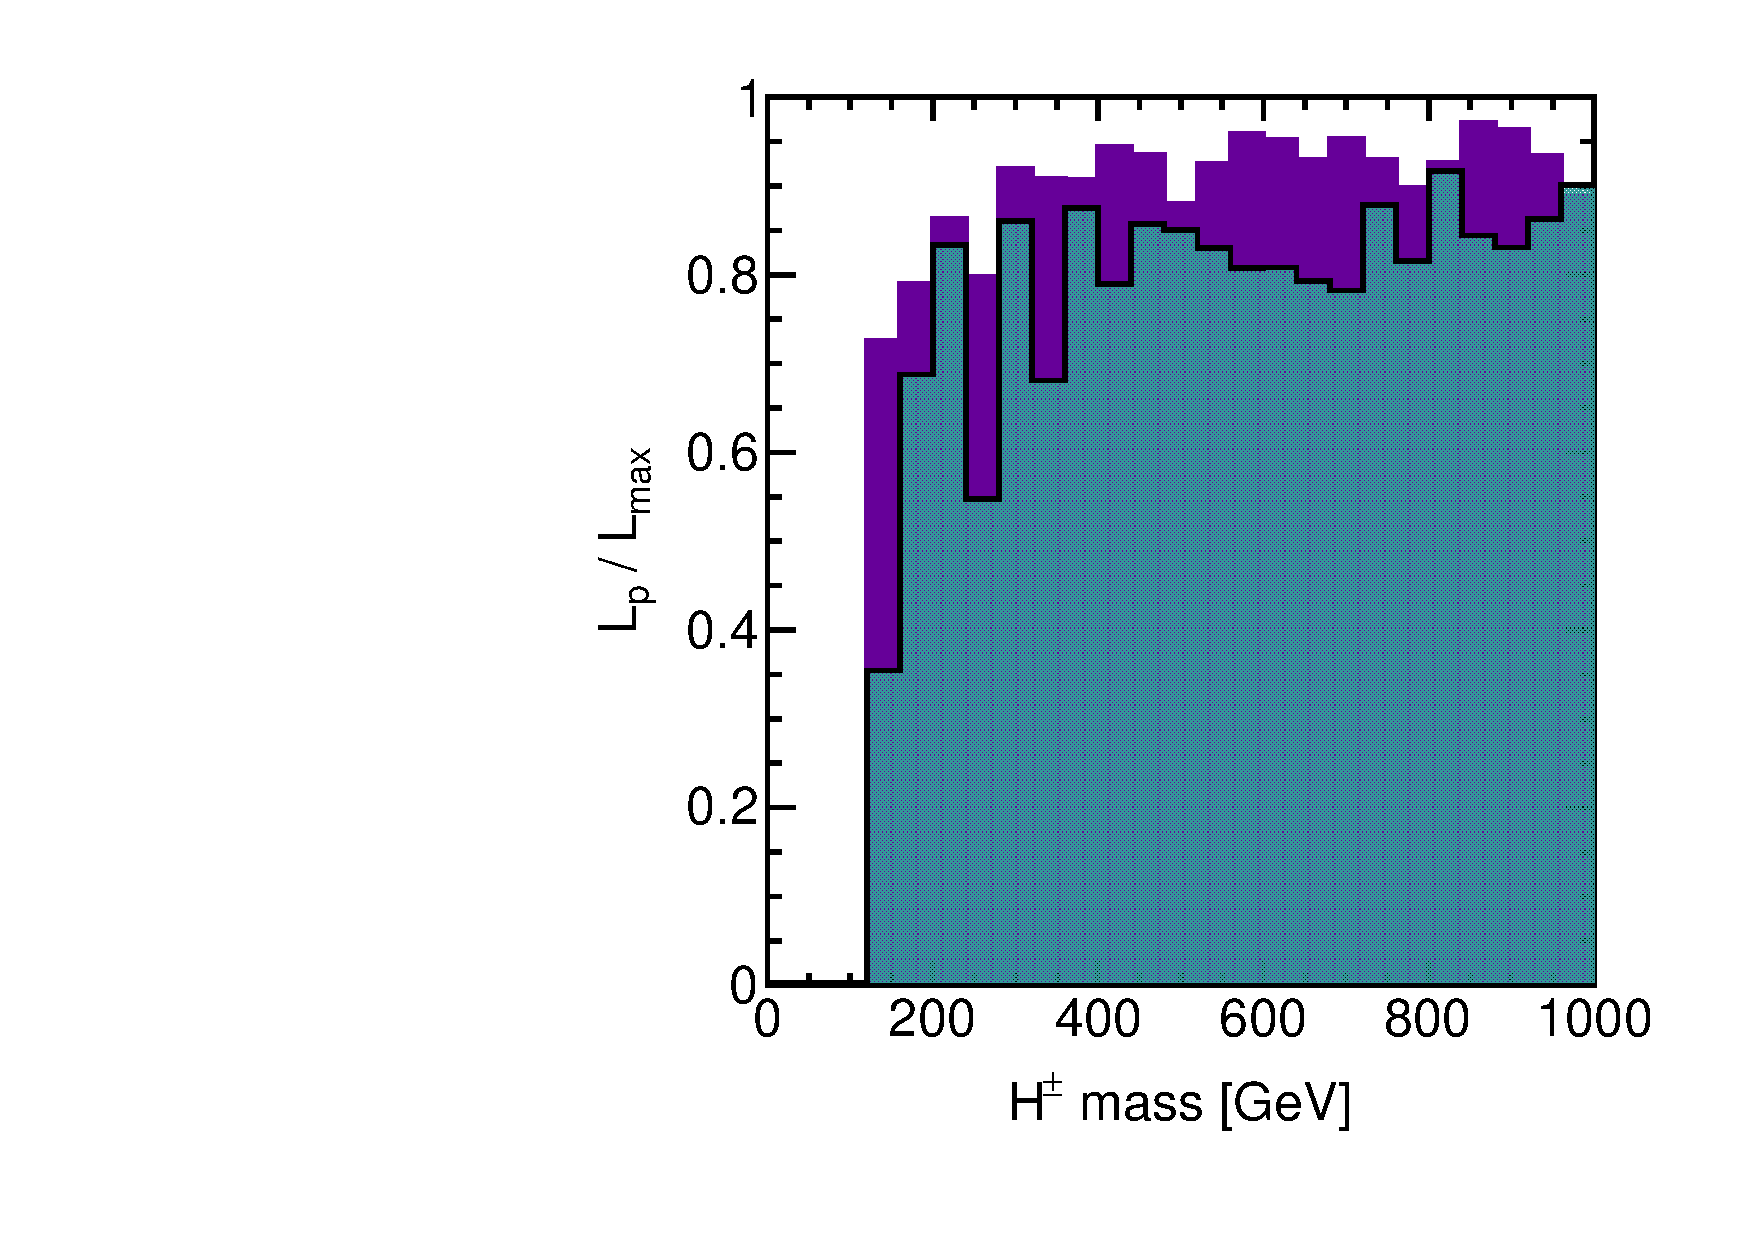
\includegraphics[height=5.5cm]{figs/fig_H_pm.pdf} 
\caption{Higgs masses}
\label{default}
\end{center}
\end{figure}


\begin{figure}[htbp]
\begin{center}
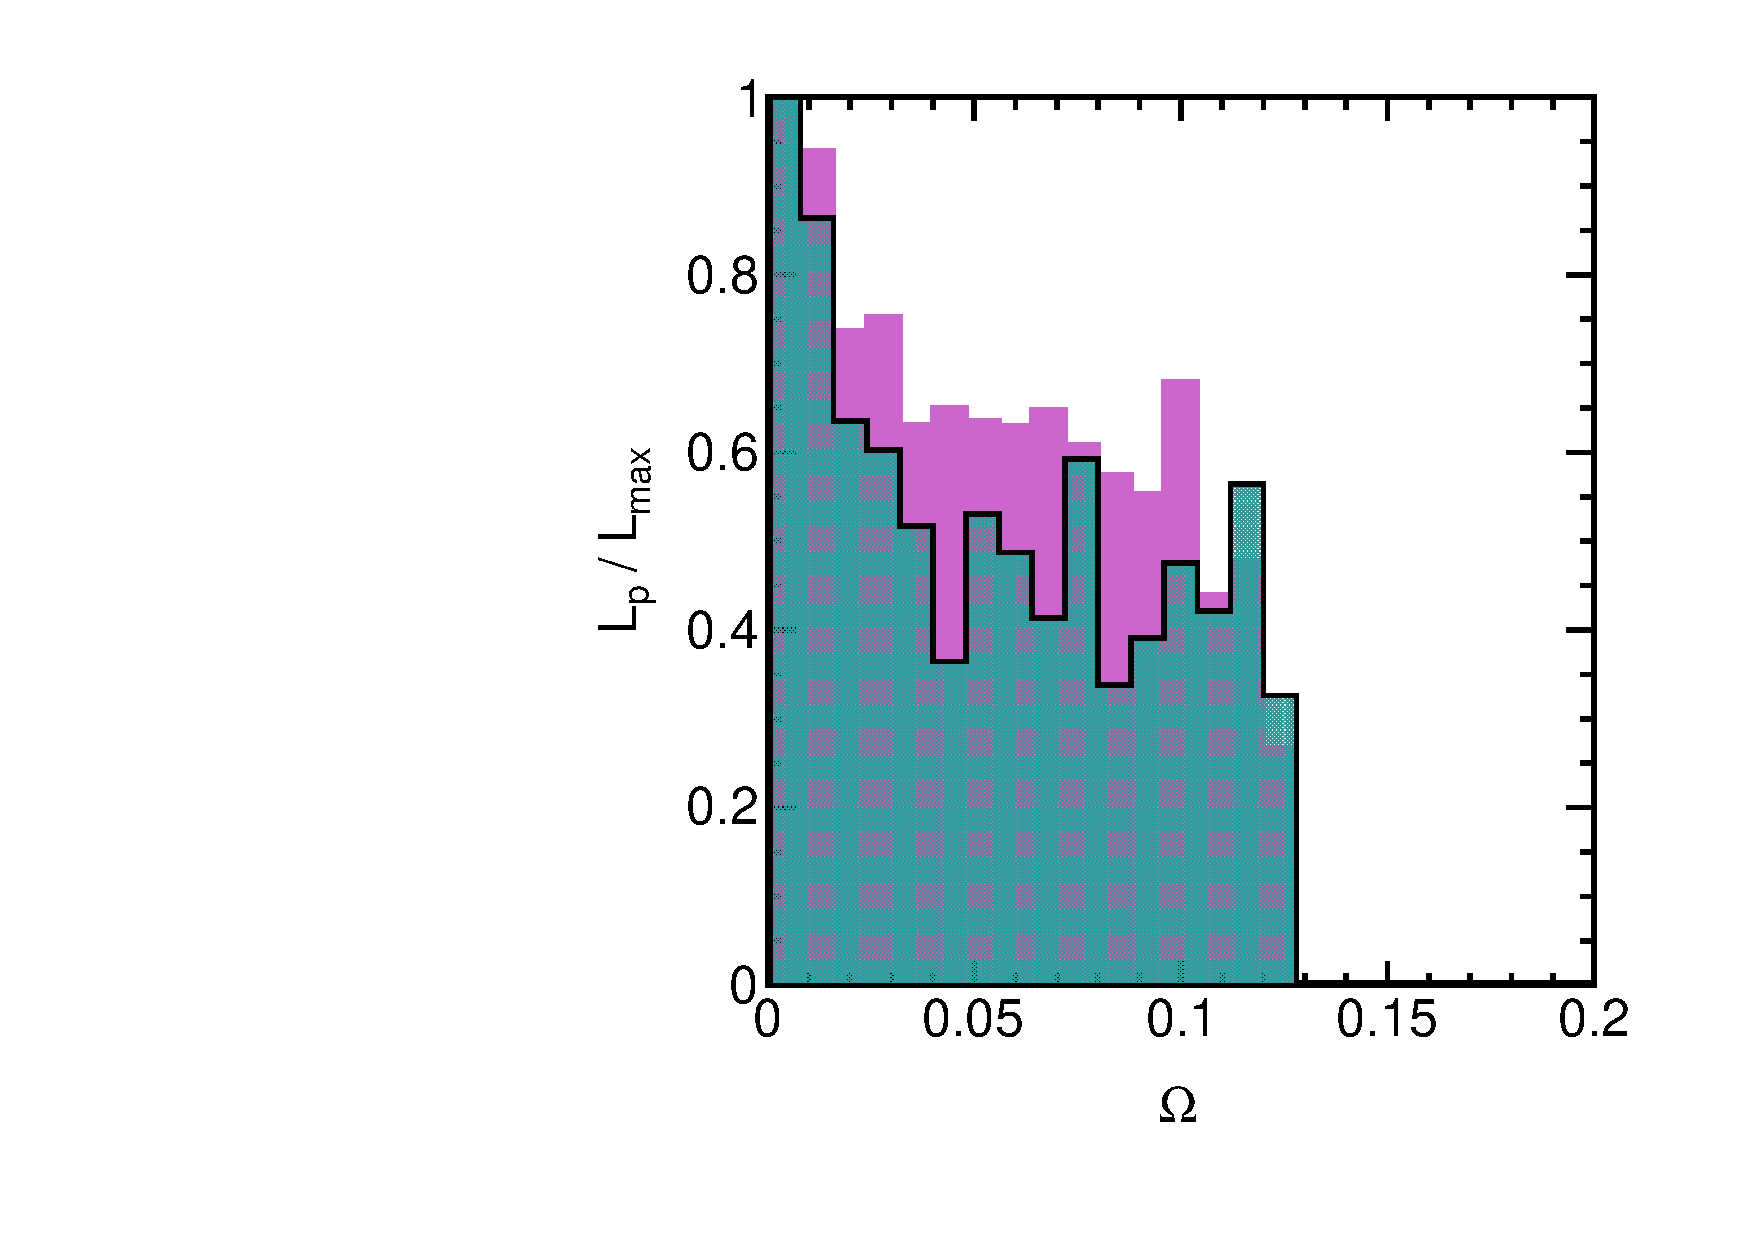
\includegraphics[height=5.5cm]{figs/fig_omega_m.pdf} 
\caption{Lightest neutralino dark matter relic density.}
\label{default}
\end{center}
\end{figure}


\begin{figure}[htbp]
\begin{center}
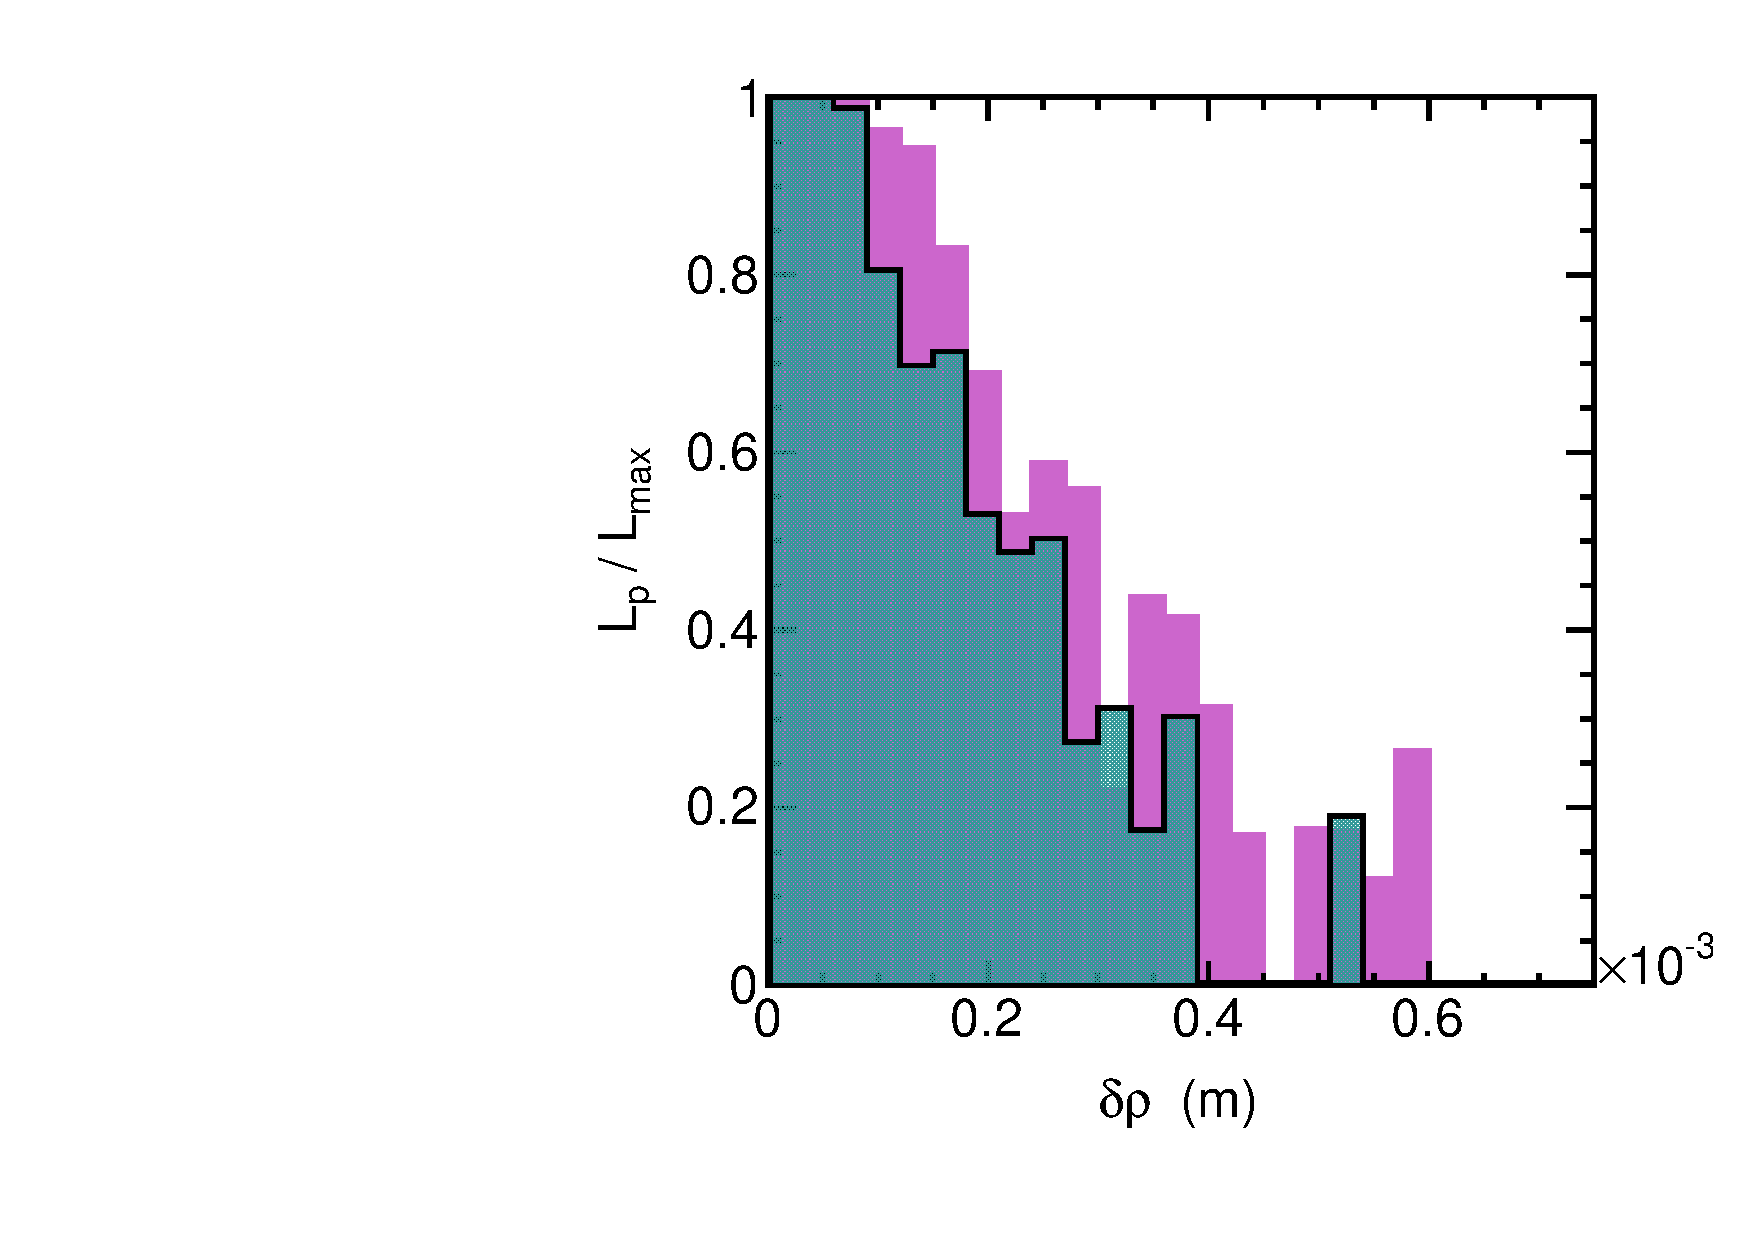
\includegraphics[height=5.5cm]{figs/fig_drho_m.pdf} 
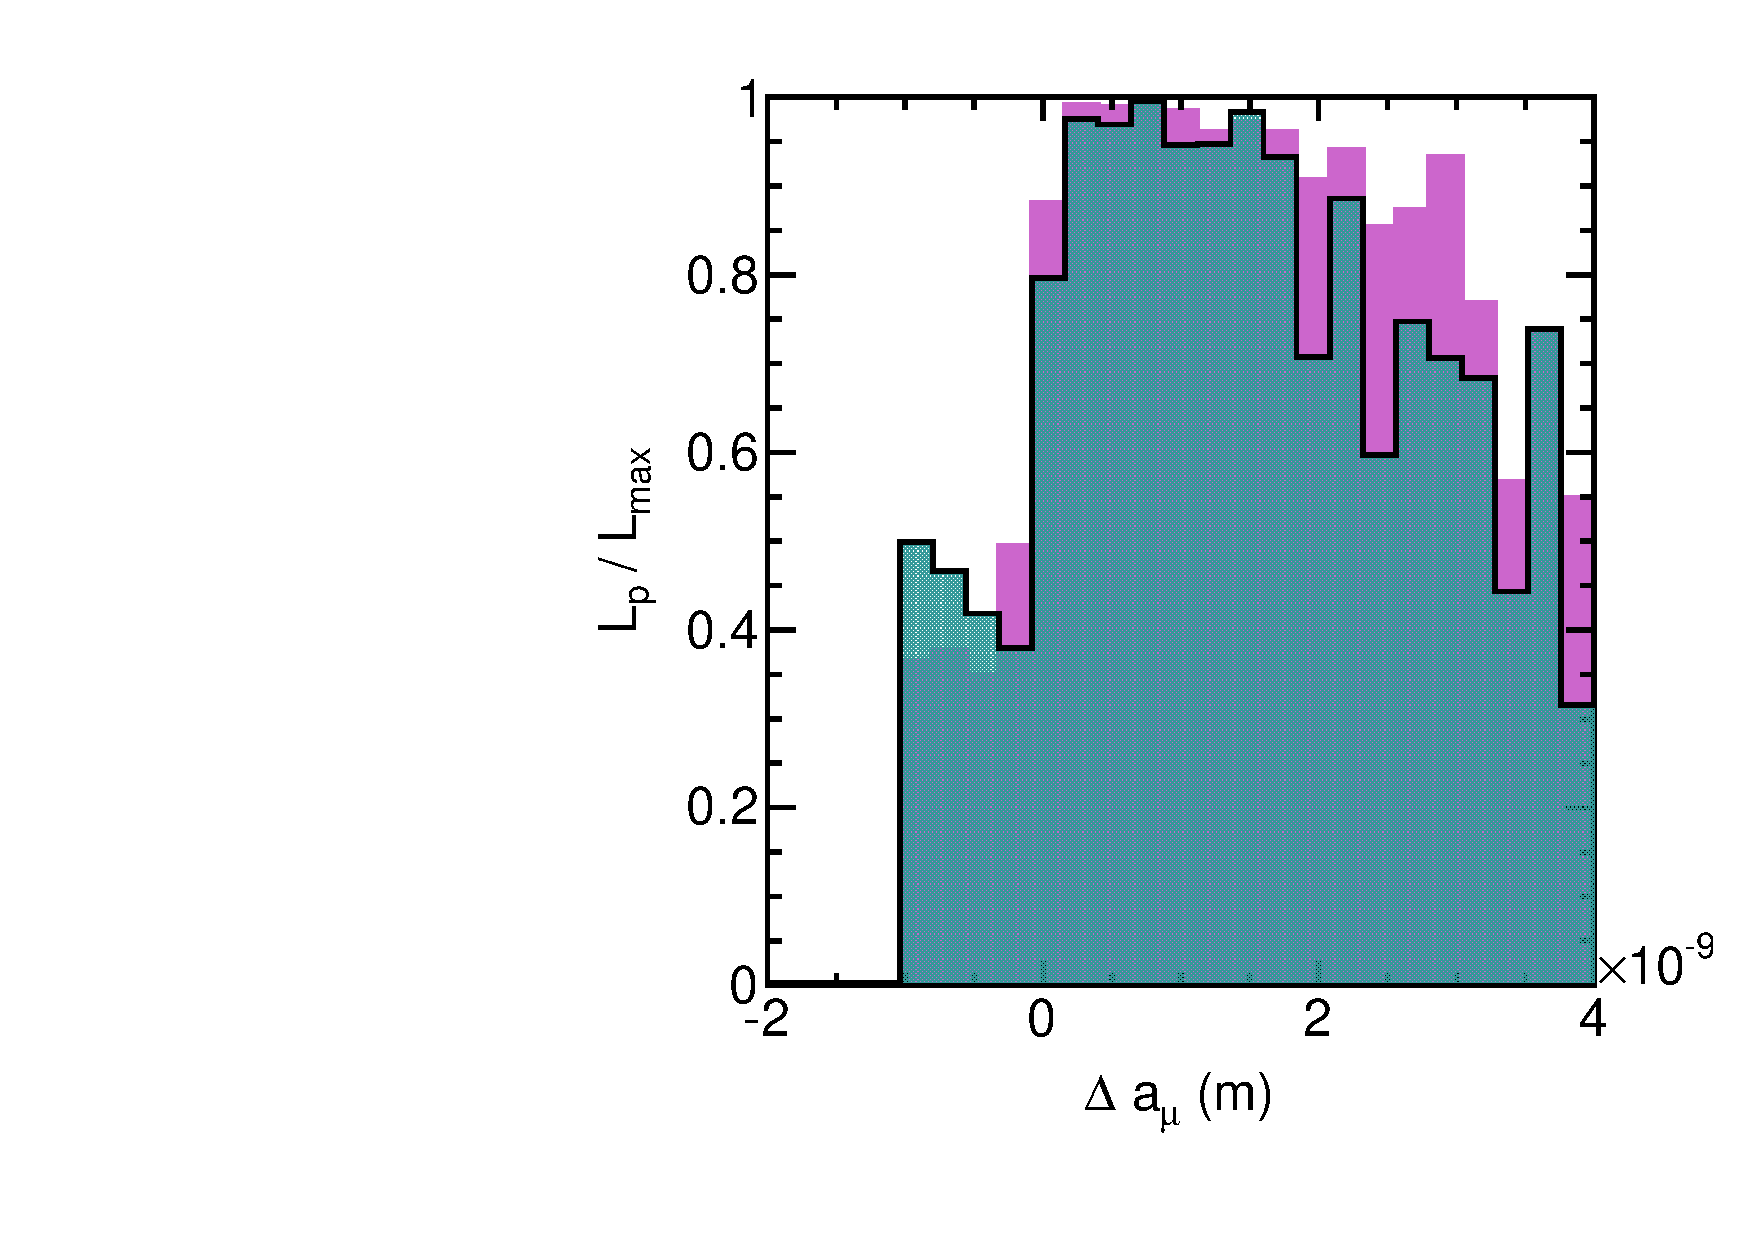
\includegraphics[height=5.5cm]{figs/fig_gmu_m.pdf} \\
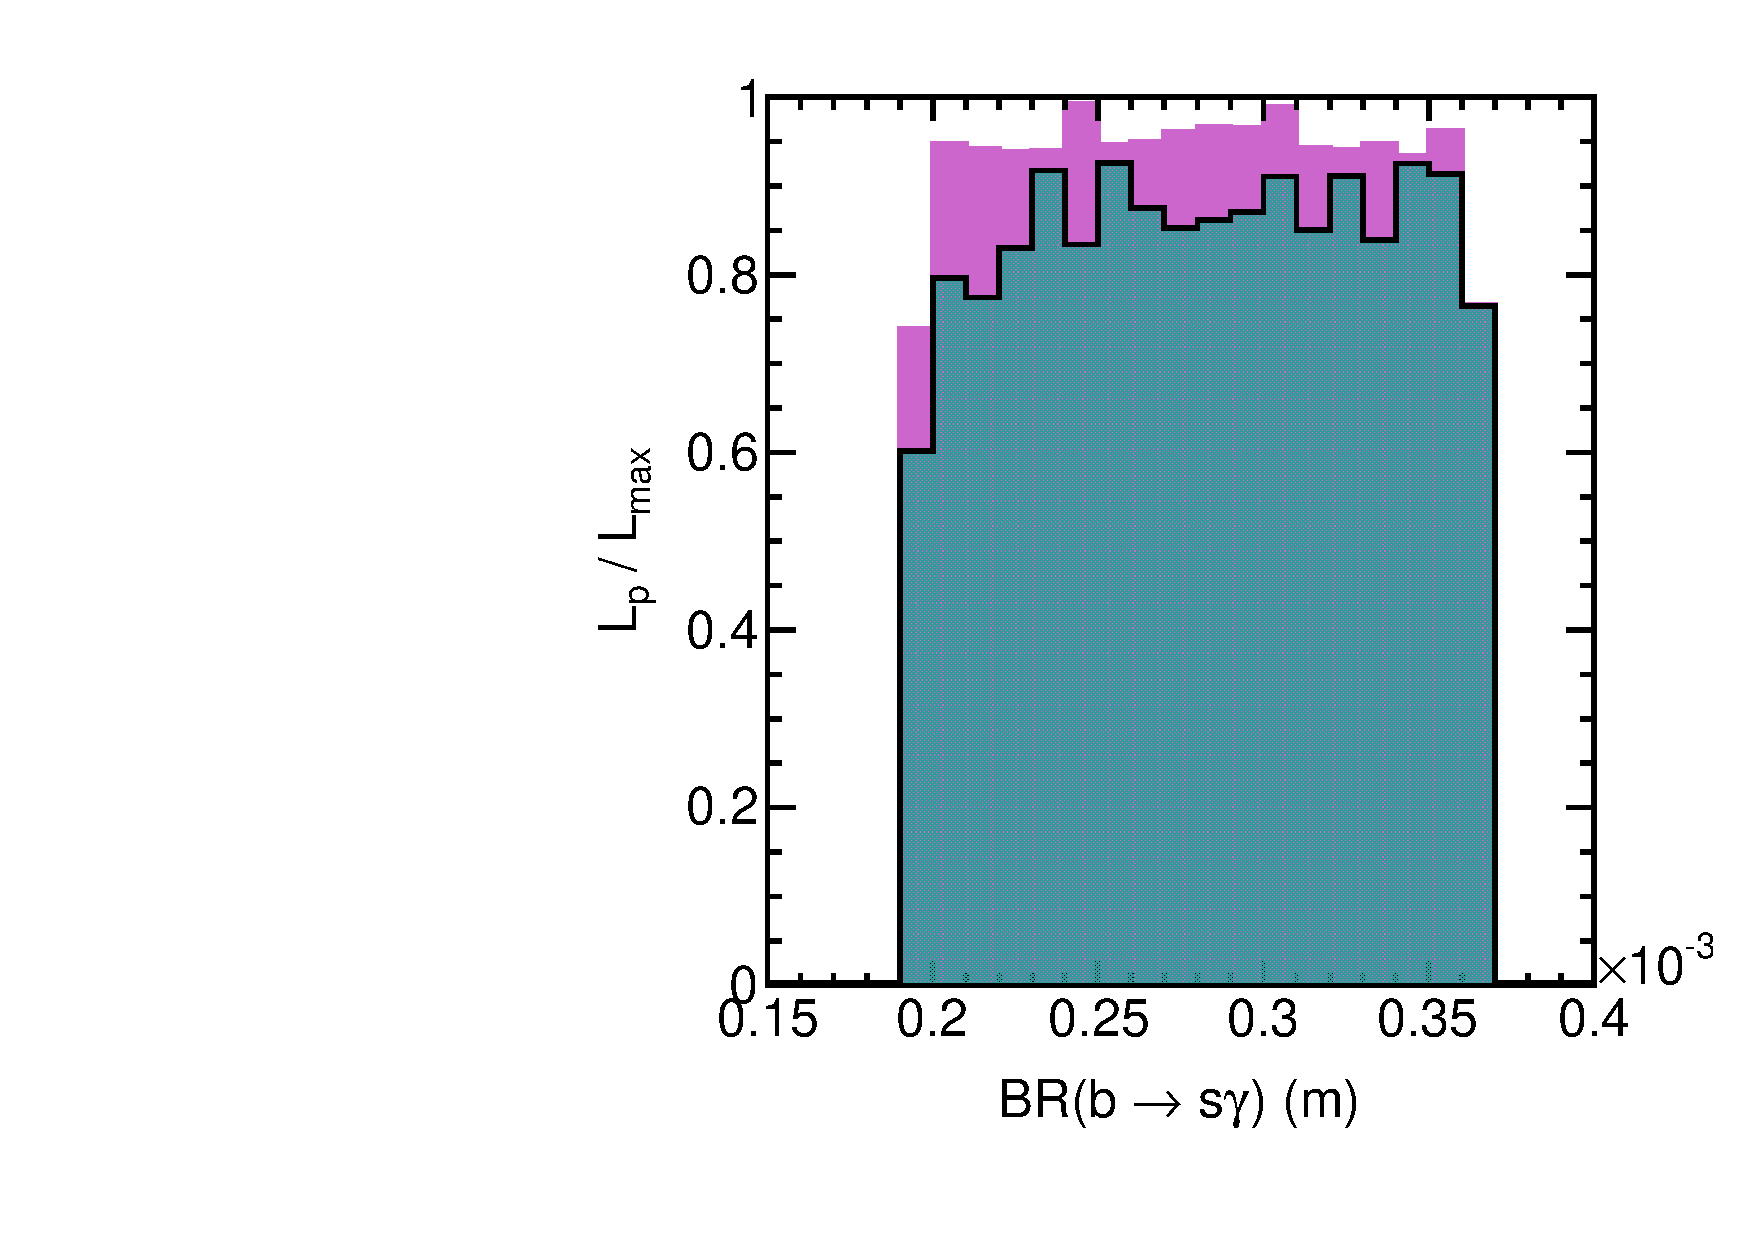
\includegraphics[height=5.5cm]{figs/fig_bsgamma_m.pdf} 
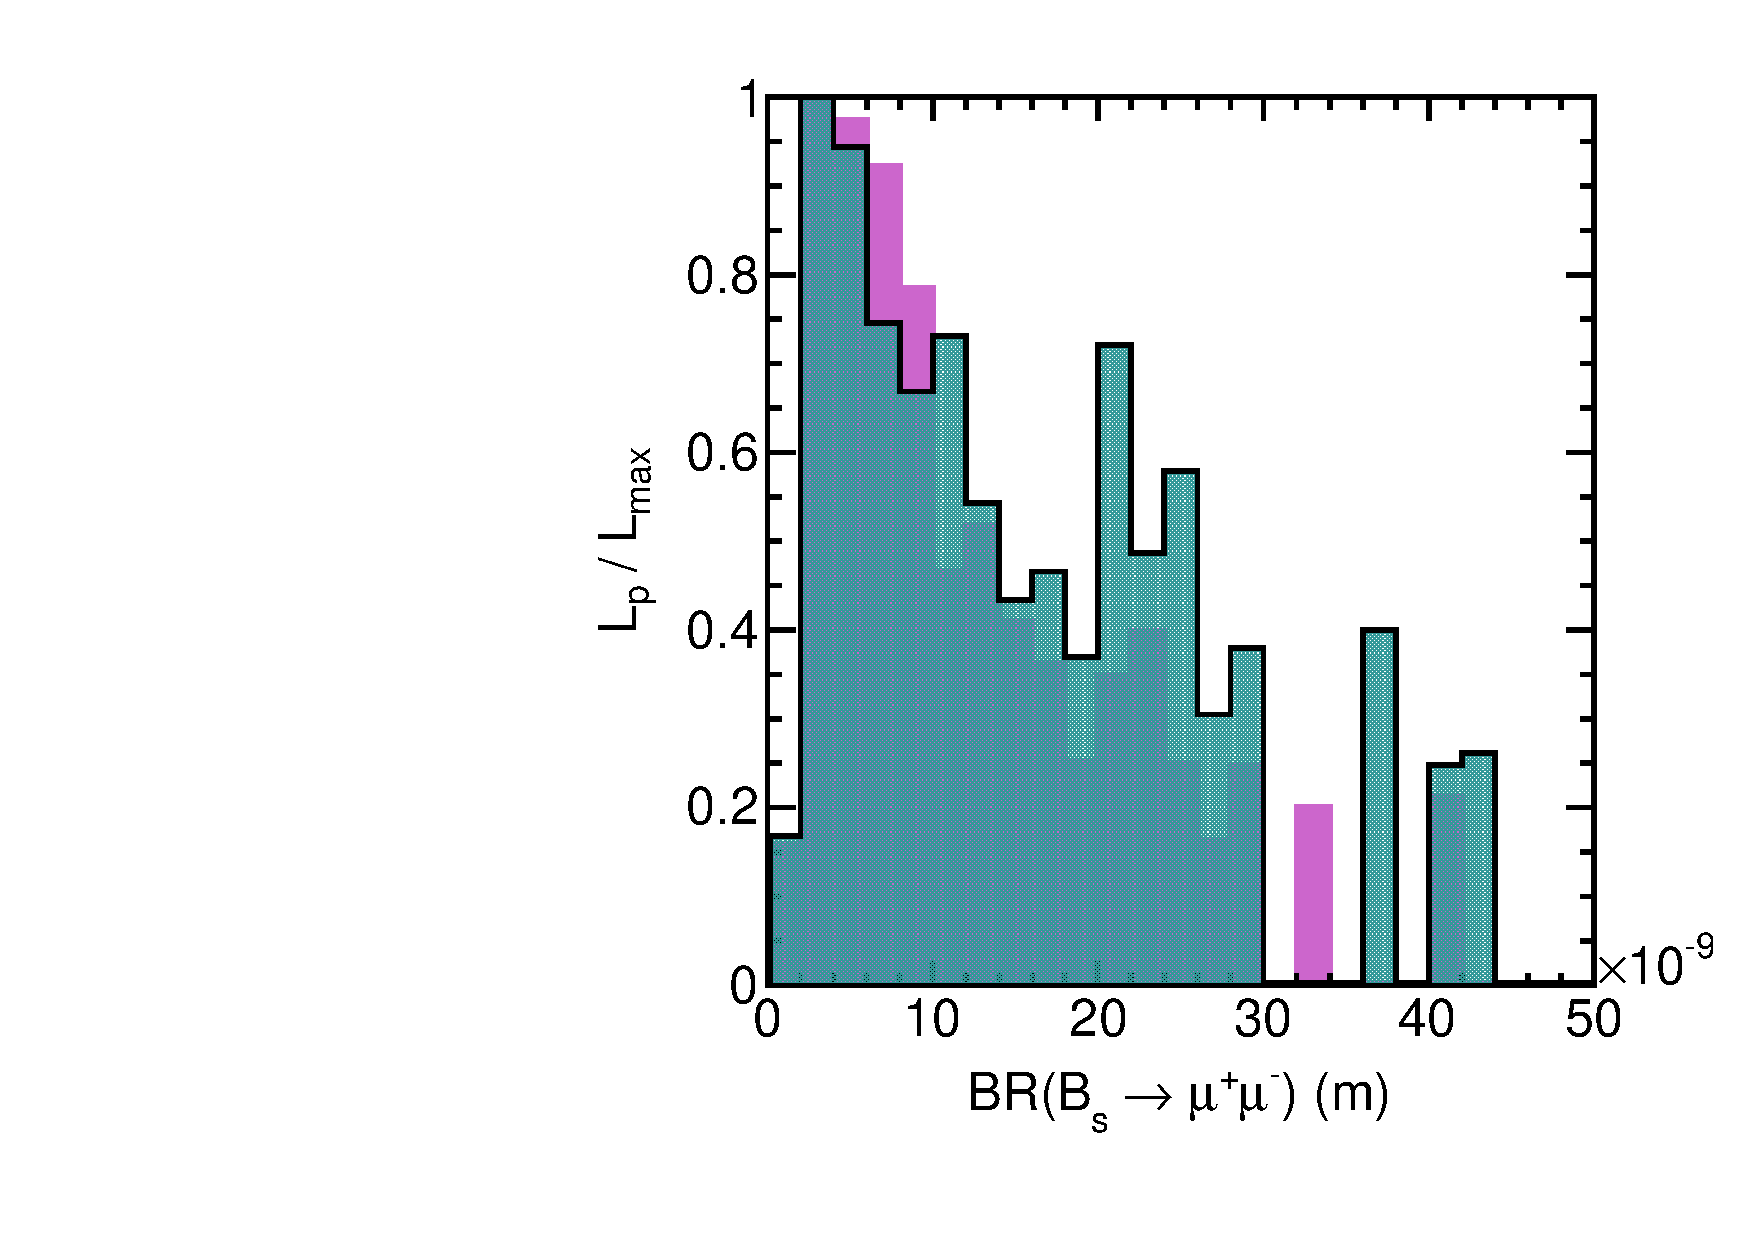
\includegraphics[height=5.5cm]{figs/fig_bsmumu_m.pdf} \\
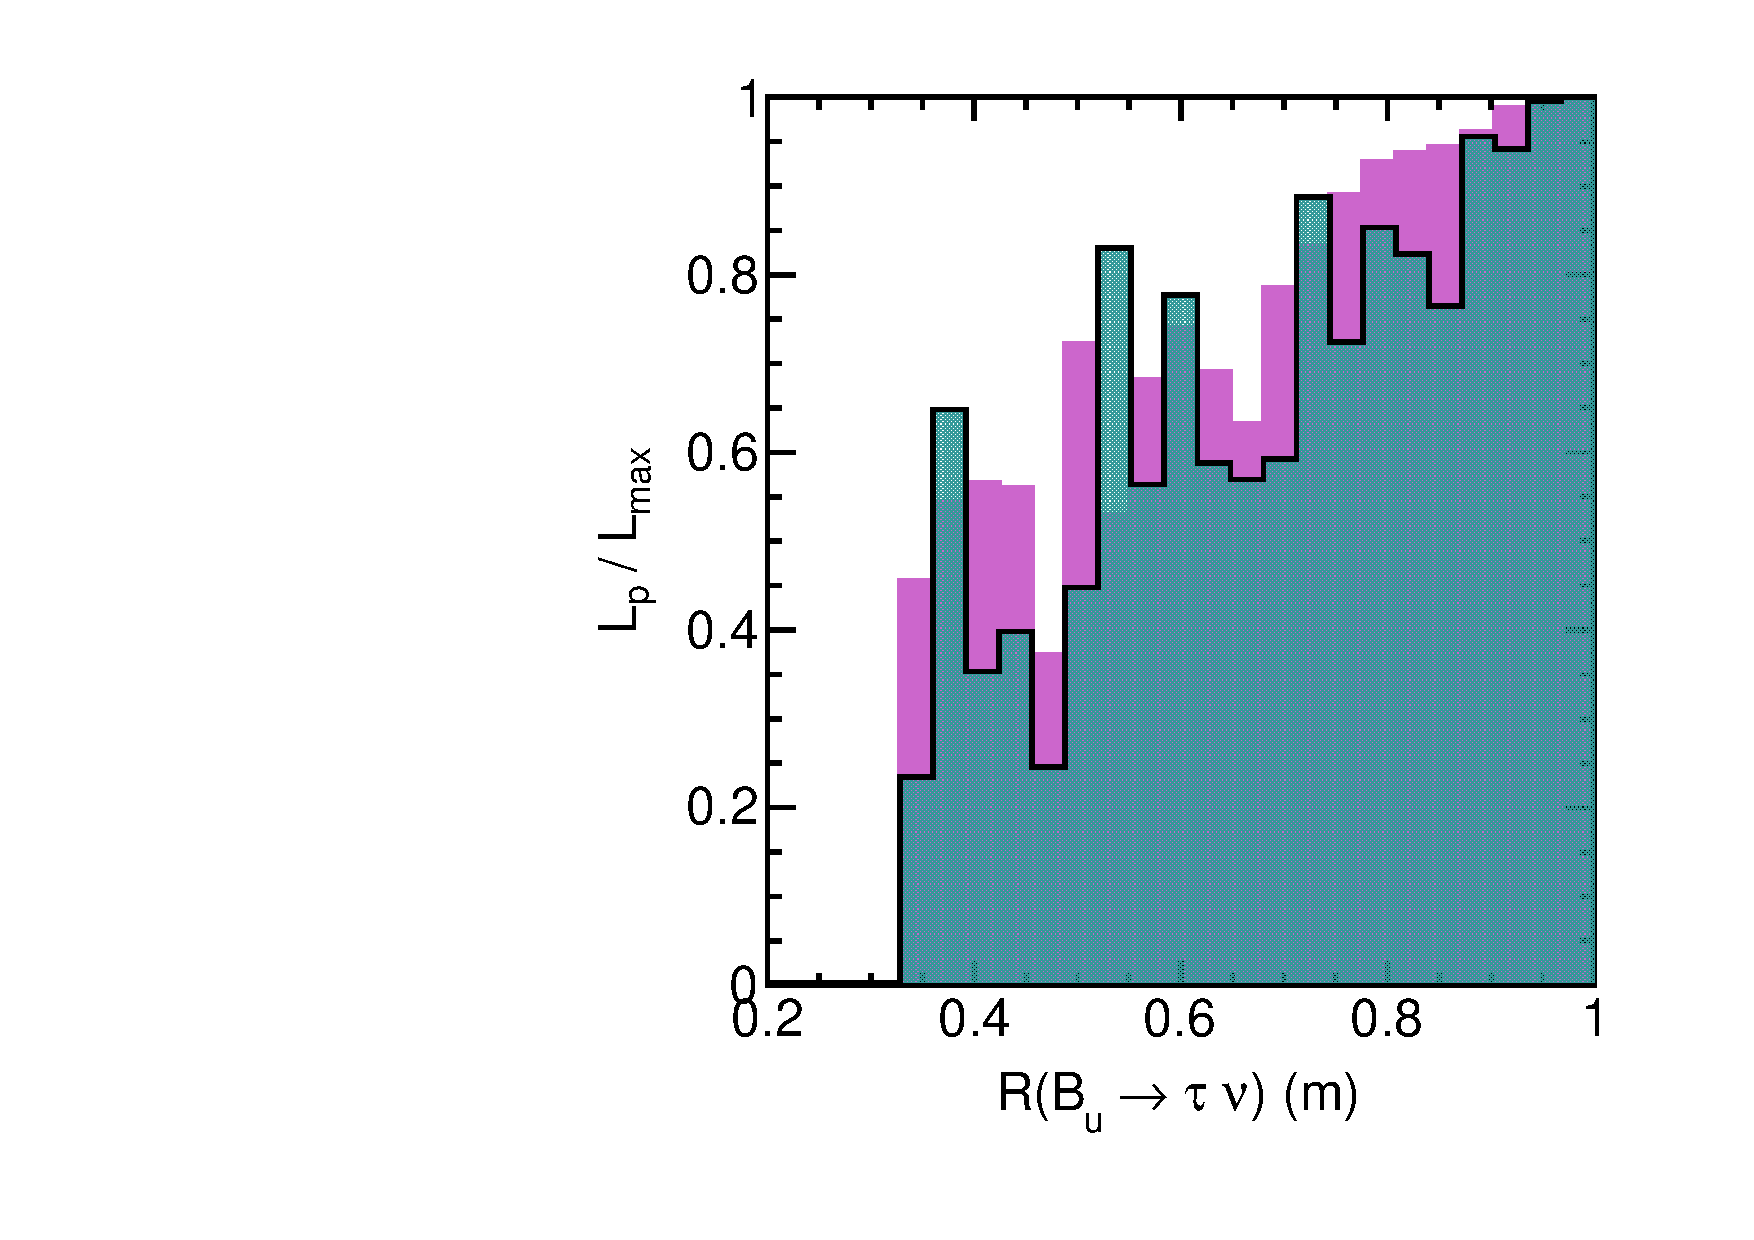
\includegraphics[height=5.5cm]{figs/fig_rbtaunu_m.pdf} 
\caption{Predictions for weak scale observables as calculated by micromegas.}
\label{default}
\end{center}
\end{figure}


\begin{figure}[htbp]
\begin{center}
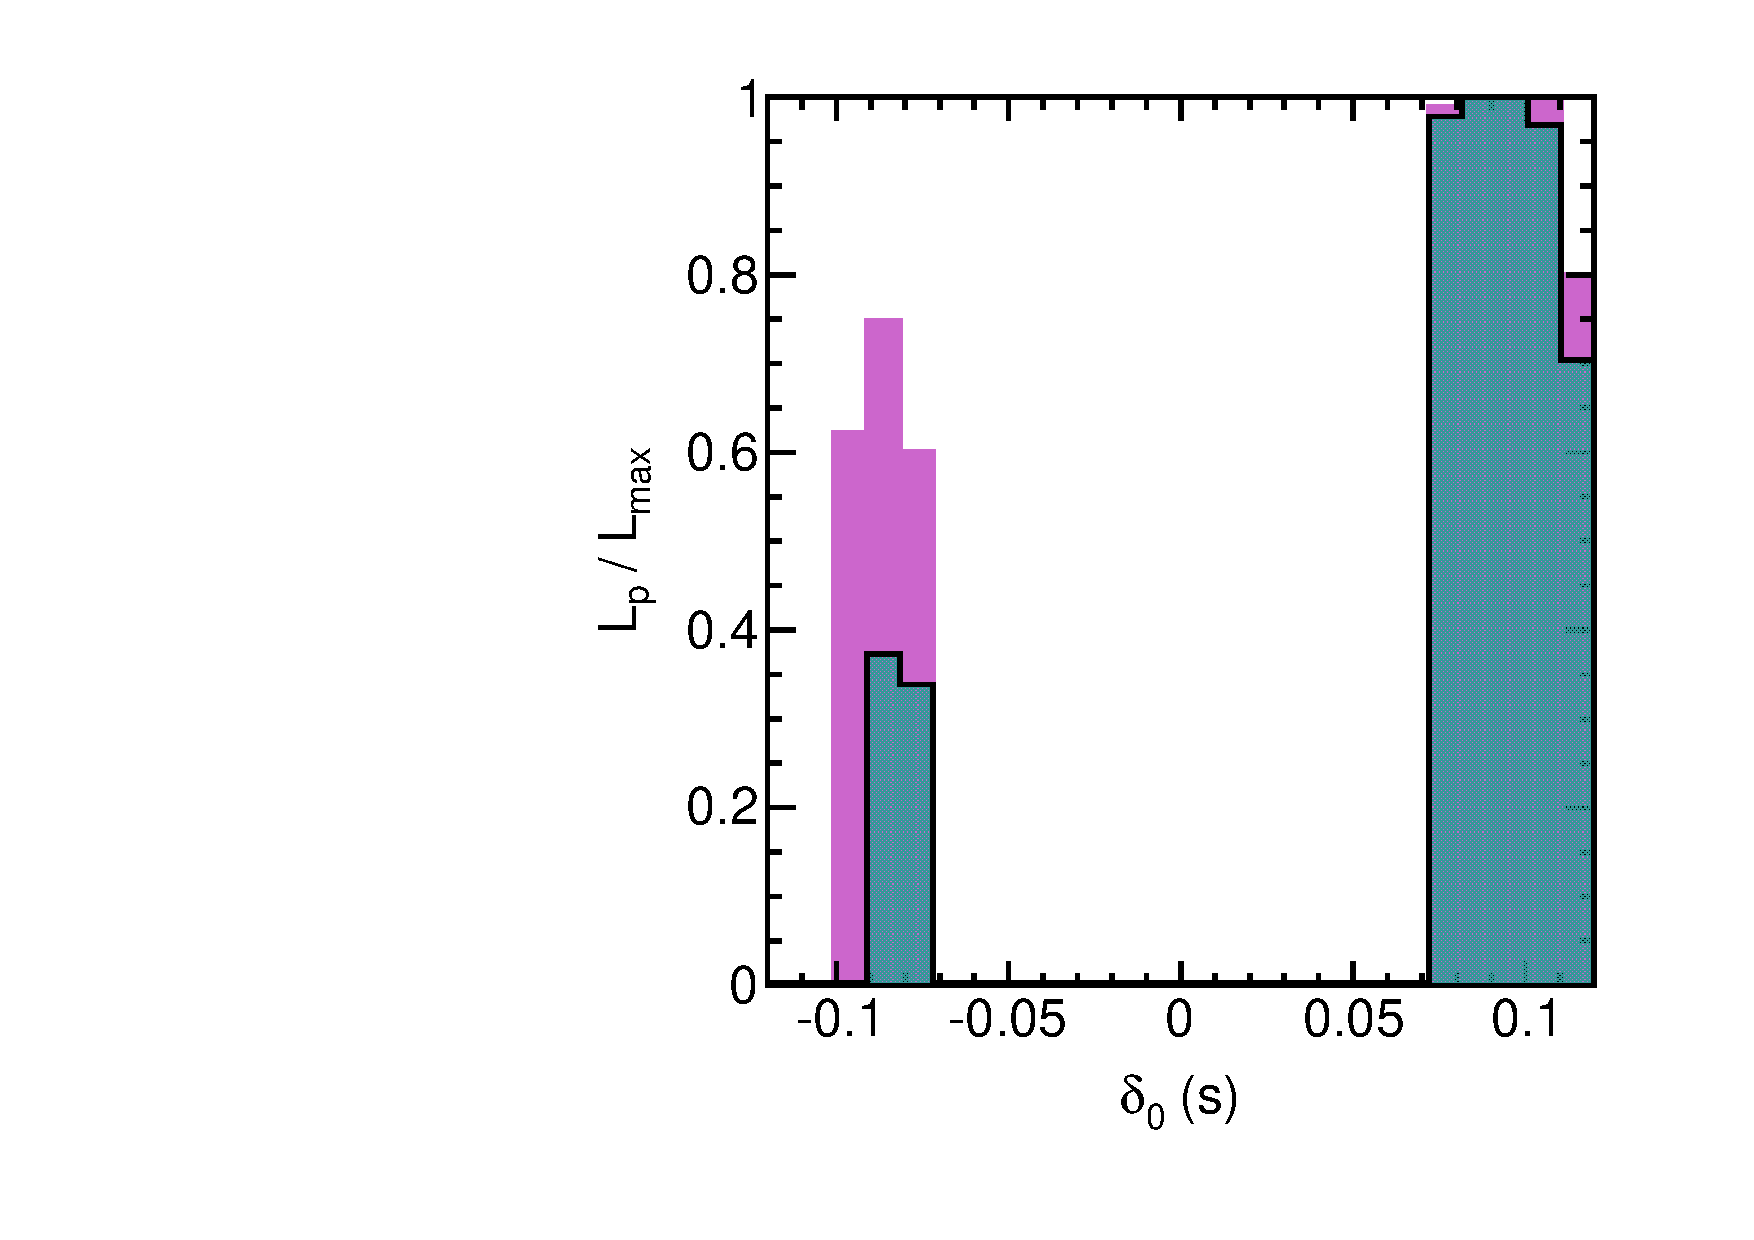
\includegraphics[height=5.5cm]{figs/fig_delta0_s.pdf} 
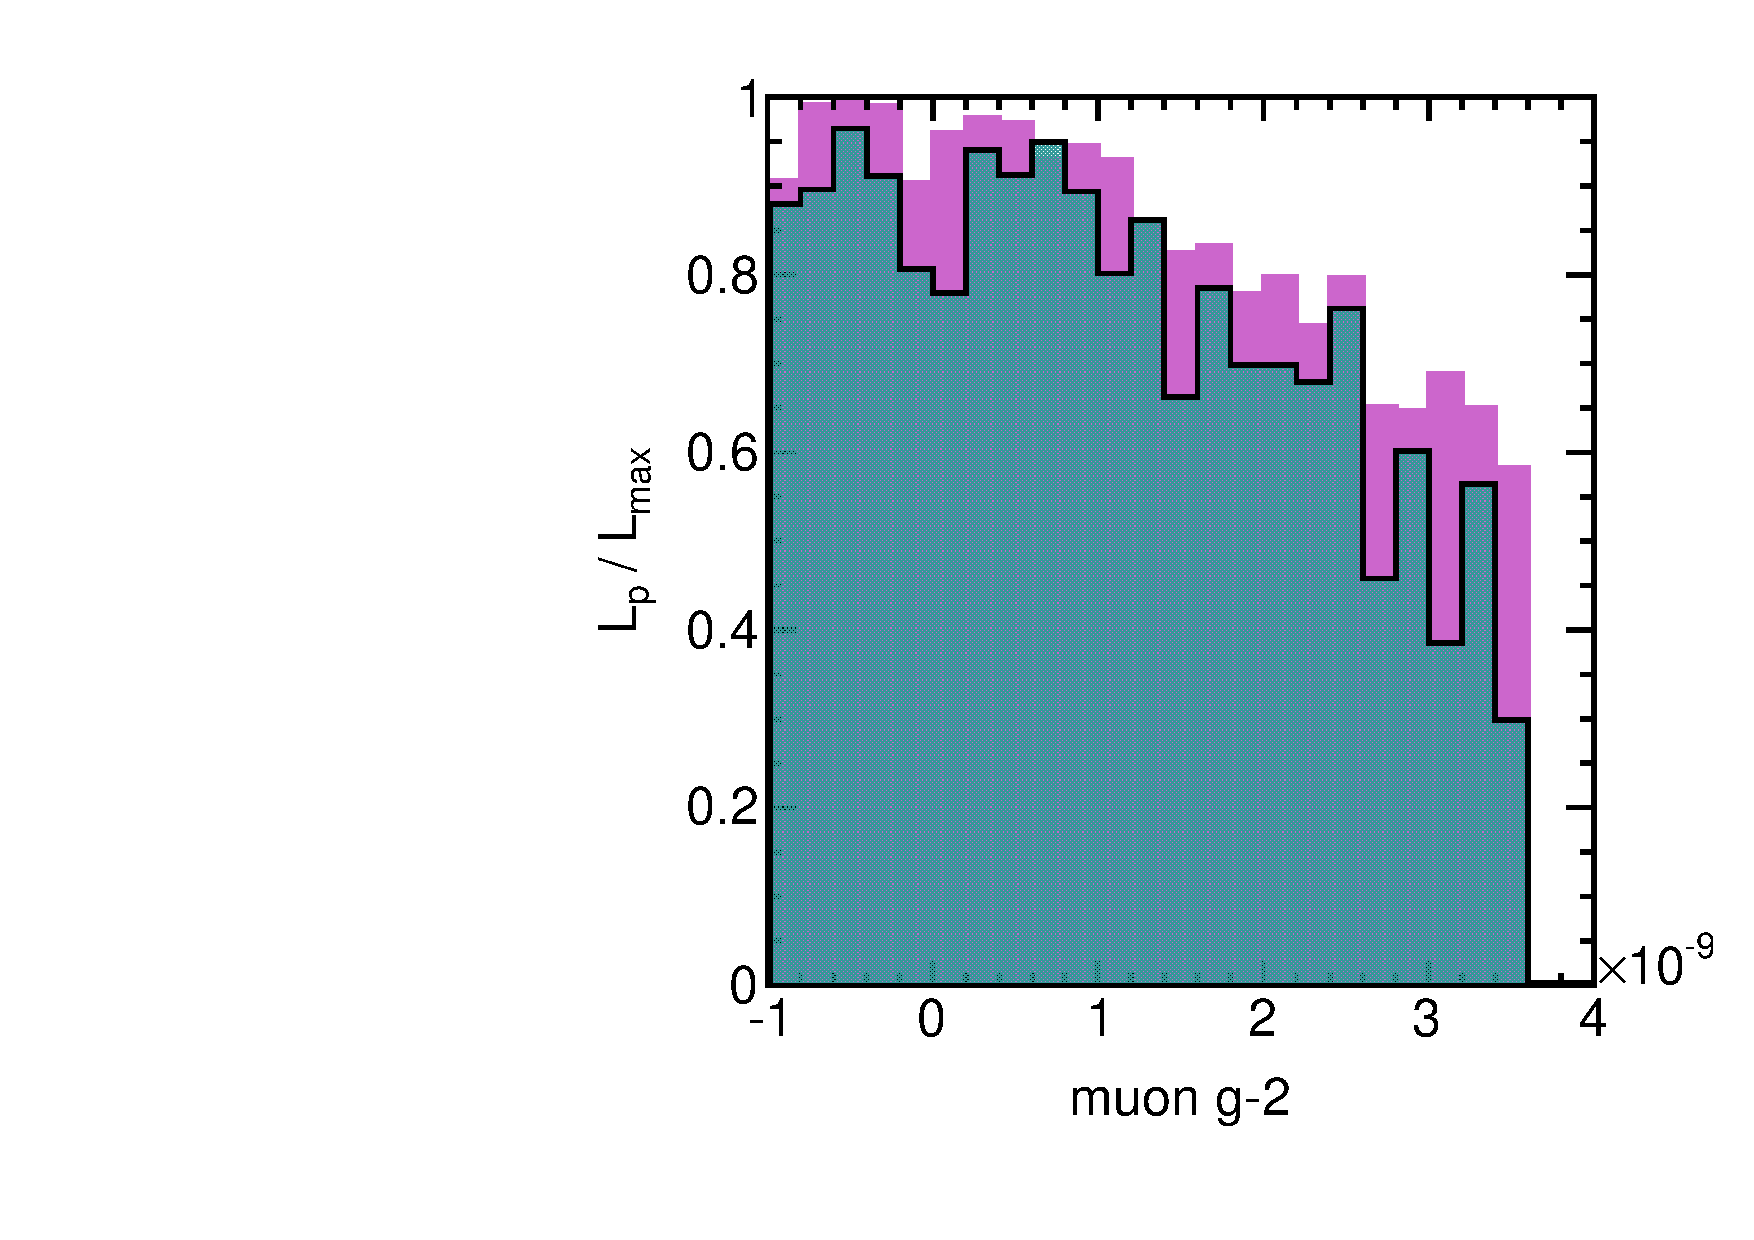
\includegraphics[height=5.5cm]{figs/fig_muon_gm2_s.pdf} \\
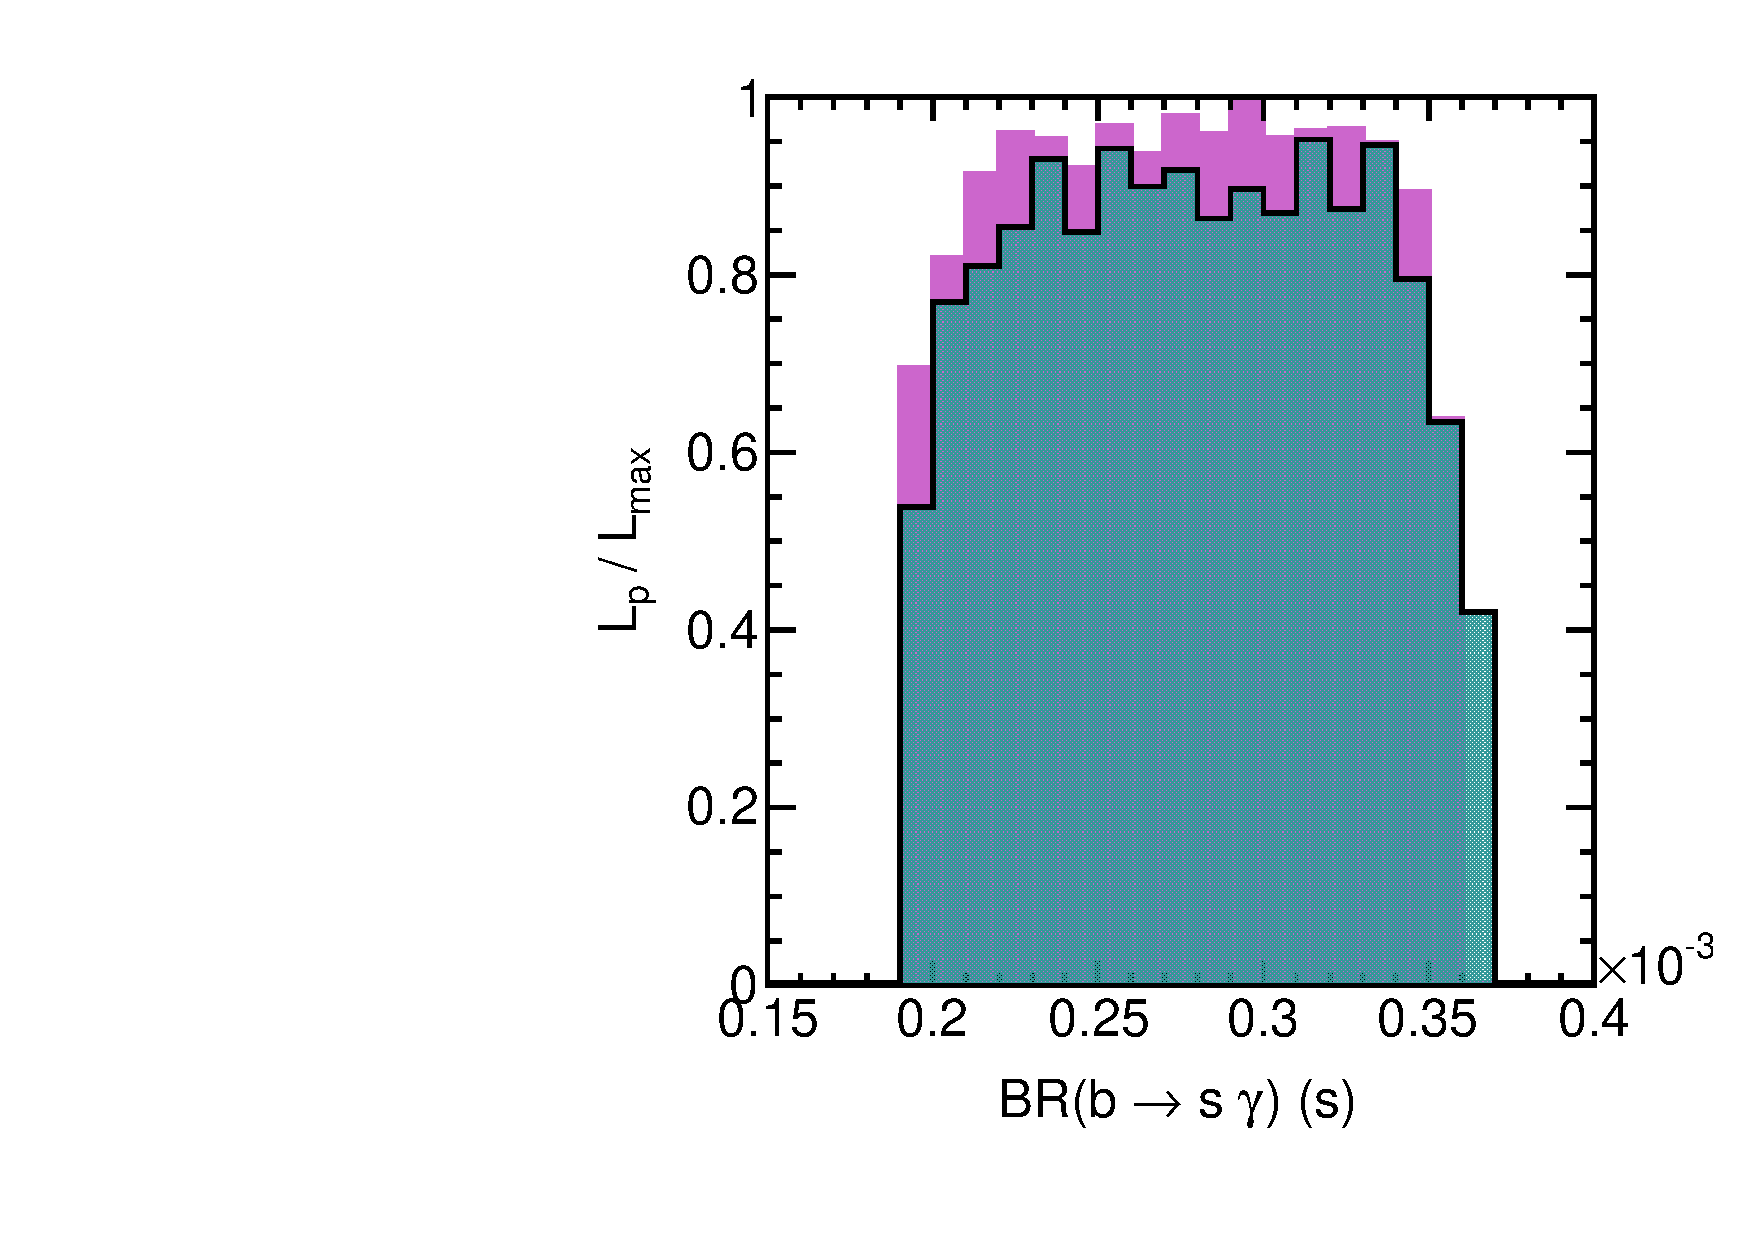
\includegraphics[height=5.5cm]{figs/fig_bsgamma_s.pdf} 
\includegraphics[height=5.5cm]{figs/fig_Bsmumu_s.pdf} \\
\includegraphics[height=5.5cm]{figs/fig_Btaunu_s.pdf} 
\includegraphics[height=5.5cm]{figs/fig_RBtaunu_s.pdf} 
\caption{Predictions for weak scale observables as calculated by superiso - I}
\label{default}
\end{center}
\end{figure}


\begin{figure}[htbp]
\begin{center}
\includegraphics[height=5.5cm]{figs/fig_BDtaunu_s.pdf} 
\includegraphics[height=5.5cm]{figs/fig_BDtaunu_BDenu_s.pdf} \\
\includegraphics[height=5.5cm]{figs/fig_Dmunu_s.pdf} 
\includegraphics[height=5.5cm]{figs/fig_Dsmunu_s.pdf} \\
\includegraphics[height=5.5cm]{figs/fig_Dstaunu_s.pdf} 
\includegraphics[height=5.5cm]{figs/fig_Kmunu_pimunu_s.pdf} \\
\includegraphics[height=5.5cm]{figs/fig_Rl23_s.pdf} 
\caption{Predictions for weak scale observables as calculated by superiso - II}
\label{default}
\end{center}
\end{figure}





